\chapter{Equilibrio Estelar Newtoniano}\label{chap:eq_newton}

\section{Ecuaciones de equilibrio}
Consideremos modelar una estrella como una distribuci'on \textit{esf'erica y est'atica de un fluido ideal no relativista en equilibrio}, esto es, como aquella situaci'on en la que la presi'on $P_{mat}$ que ejerce la materia hacia el exterior (debida, por ejemplo, a reacciones termonucleares)  es capaz de mantener el equilibrio de la estrella, contrarrestando su propia
atracci'on gravitacional, que tiende a comprimirla.

Como estamos considerando un fluido ideal, sin viscosidad, la ecuaci'on de Euler adopta la siguiente forma para el campo de velocidades $\vec{v}$:

\begin{equation}\label{euler}
\rho(\vec{r})\frac{d\vec{v}}{dt}=\rho(\vec{r})\left( \dfrac{\partial\vec{v}}{\partial t}+(\vec{v}\cdot\vec{\nabla})\vec{v}\right)=-\vec{\nabla}P(\vec{r})+\vec{f} (\vec{r}).
\end{equation}
En el caso est'atico considerado el campo velocidad ser'a nulo $\vec{v}(\vec{x},t)=\vec{0}$. Aqu'i $\vec{f}$ es la \textit{densidad de fuerza externa} que act'ua en cada elemento de volumen. As'i, la ec. (\ref{euler}) se reducir'a a $\vec{\nabla}P=\vec{f}$. Pero en este caso la 'unica fuerza externa considerada es la gravitacional, que act'ua sobre un elemento de masa $dm=\rho(\vec{r})dV$ con densidad $\rho(\vec{r})$, y es por lo tanto dado por $d\vec{F}_g=-dm\vec{\nabla}\phi$, donde $\phi$ es el potencial gravitacional newtoniano. De este modo, la densidad de fuerza ser'a $\vec{f}=-\rho\vec{\nabla}\phi$, y por lo tanto, la condici'on de equilibrio queda expresada por:
\begin{equation}\label{equi}
\vec{\nabla}P(\vec{r})=-\rho\vec{\nabla}\phi(\vec{r}).
\end{equation}

Al asumir \textit{simetr'ia esf'erica}, tenemos que $P=P(r)$ y $\phi=\phi(r)$, entonces
\begin{equation}\label{equir}
\frac{dP(\vec{r})}{dr}=-\rho(\vec{r})\frac{d\phi}{dr}.
\end{equation}

Por otro lado, el potencial gravitacional $\phi$ satisface la ecuaci'on de Poisson:
\begin{equation}\label{n2p}
\nabla^2\phi(r)=4\pi G\rho(r).
\end{equation}

Integrando la ecuaci'on anterior desde el centro de la estrella, $r=0$, hasta un radio arbitrario $r$,  y denotando la \textit{masa dentro del radio} $r$ de la estrella por
\begin{equation}\label{masa1}\marginnote{Ecuaci'on de masa}
\mathcal{M}(r)=4\pi\int\limits^r_{0}dr'r'^2\rho(r'),
\end{equation}
o, equivalentemente
\begin{equation}\label{masa2}\marginnote{Ecuaci'on de masa como derivada}
\boxed{\frac{d\mathcal{M}(r)}{dr}=4\pi r^2\rho(r),}
\end{equation}
tenemos luego que \eqref{n2p} implica (asumiendo que \textit{no existe} una masa puntual en el centro):
\begin{equation}
\frac{d\phi}{dr}=\frac{4\pi G}{r^2}\int\limits^r_{0}dr'r'^2\rho(r')=\frac{G\mathcal{M}(r)}{r^2}.
\end{equation}

Reemplazando la expresi'on anterior en (\ref{equir}), tenemos la condici'on de equilibrio hidrost'atico newtoniano:
\begin{equation}\label{eqnewton}\marginnote{Equilibrio hidrost'atico newtoniano}
\boxed{\frac{dP(r)}{dr}=-\frac{G\mathcal{M}(r)}{r^2}\rho(r).}
\end{equation}

Notemos que, debido a que $\rho>0$, \textbf{la presi'on es una funci'on mon'otonamente decreciente de la coordenada radial}.


\section{Resolviendo las ecuaciones de estructura}\label{resolviendo}

La ecuaci'on de equilibrio hidrost'atico (\ref{eqnewton}) y la ecuaci'on de masa, (\ref{masa1}) 'o (\ref{masa2}), conforman un sistema de \textit{dos ecuaciones} en las que hay \textit{tres campos escalares}, dependientes de la coordenada radial, por determinar: la presi'on $P(r)$, la densidad $\rho\,(r)$ y la masa $\mathcal{M}(r)$. Por lo tanto, necesitamos otra ecuaci'on que ligue a las variables anteriores para que exista una soluci'on 'unica a una determinada configuraci'on. Usualmente, esta ecuaci'on faltante liga a la presi'on con la densidad (cuando la entrop'ia $s$ es constante) y se conoce como \emph{ecuaci'on de estado}\footnote{Para mayores detalles, ver ap'endice  \ref{cap:termo}.}:
\begin{equation}\label{estado}\marginnote{Ecuaci'on de estado}
\boxed{P=P(\rho).}
\end{equation}

As'i, tenemos un sistema de dos ecuaciones diferenciales y una ecuaci'on algebraica para la estructura estelar, que adoptan la forma
\begin{align}
 P'(r)&=P'(P(r),\mathcal{M}(r)),\\
\mathcal{M}'(r)&=\mathcal{M}(\rho(r)),\\
P(r)&=P(\rho(r)).
\end{align}

Luego, el sistema f'isico modelado por el sistema de ecuaciones (\ref{eqnewton}), (\ref{masa2}) y (\ref{estado}) quedar'a completamente determinado imponiendo dos condiciones iniciales apropiadas (tenemos dos ecuaciones diferenciales de primer orden):
\begin{enumerate}
 \item $\mathcal{M}(r=0)=0$. Esto suceder'a siempre que $\rho(r=0)$ sea \textit{finito}, como es razonable suponer.
 \item $P(r=0)=P_0$. Se asigna un valor dado a la presi'on en el centro de la estrella.
\end{enumerate}

Como la presi'on \marginnote{Procedimiento de \\resoluci'on} es una funci'on mon'otonamente decreciente (puesto que $\rho(r)\geq0$), la determinaci'on de un modelo estelar $[P(r), \rho(r),\mathcal{M}(r)]$, dada una ecuaci'on de estado y una cierta presi'on central, se obtendr'a integrando el sistema de ecuaciones antes mencionado desde el centro hacia afuera, hasta llegar a un punto $r=R$ tal que $P(r=R)=0$. A dicha coordenada $R$ se le denominar'a \textit{radio de la estrella}. Aqu'i se debe considerar la imposici'on f'isica que $(\forall\; r\geq R) \quad P=0 \quad\mbox{y}\quad \rho=0$. Evaluando la ecuaci'on (\ref{masa1}) en el radio $R$, definiremos \textit{la masa total $M$ de la estrella}  como
\begin{equation}\marginnote{Masa total}
M:=\mathcal{M}(r=R).
\end{equation}



\section{Soluci'on: Densidad constante}
\subsection{Obteniendo la presi'on  \texorpdfstring{$P(r)$}{P(r)}}
El caso m'as simple de resolver el sistema de ecuaciones de equilibrio estelar es asumir la ecuaci'on de estado para densidad constante,
\begin{equation}\label{cte0}
\rho=\rho_{\rm c}=cte,\quad r\leq R,
\end{equation}
i.e., considerar materia incompresible. 'Esta es una suposici'on poco realista, pero el modelo estelar as'i construido ya muestra muchas de las caracter'isticas de otros m'as complejos.

Con dicha ecuaci'on de estado, es posible integrar directamente la ecuaci'on de masa (\ref{masa1}):

\begin{equation}\label{cte1}
\mathcal{M}(r)=4\pi\int^r_{0}dr'r'^2\rho_{\rm c}=4\pi\rho_{\rm c}\int^r_{0}dr'r'^2=\frac{4}{3}\pi\rho_{\rm c} r^3.
\end{equation}

Luego, reemplazando lo anterior en la ecuaci'on de equilibrio hidrost'atico (\ref{eqnewton}) e integrando de $r=0$ a $r=r$ (recordar que $P(r=0)=P_0$ es la presi'on central), obtenemos
\begin{align*}
 \frac{dP(r)}{dr}&=-\frac{G\mathcal{M}(r)}{r^2}\rho_{\rm c}=-\frac{4}{3}\pi G\rho_{\rm c}^2 r,
\end{align*}
y por lo tanto,

\begin{equation}
\label{cte2}\boxed{P(r)=P_0-\frac{2}{3}\pi G\rho_{\rm c}^2 r^2.}
\end{equation}

\marginnote{Soluci'on \text{con $\rho=cte$}}
As'i, hemos resuelto el problema al obtener la forma expl'icita de los tres campos escalares involucrados: ver (\ref{cte0}), (\ref{cte1}) y (\ref{cte2}). Ahora podemos encontrar el radio total de la estrella en funci'on de la presi'on central, de acuerdo a la definici'on anterior ($P(R)=0$), evaluando (\ref{cte2}) en $r=R$:
\begin{equation}\label{ctep}
 P_0=\frac{2}{3}\pi G\rho_{\rm c}^2 R^2.
\end{equation}
Por otra parte, la masa total de la estrella se encuentra, de acuerdo a su definici'on, evaluando (\ref{cte1}) en $r=R$ dado por (\ref{ctep}):
\begin{equation}\label{ctem}
 M=\mathcal{M}(R)=\frac{4}{3}\pi\rho_{\rm c} R^3.
\end{equation}
Si se reemplaza (\ref{ctem}) en (\ref{ctep}) y se recuerda la definici'on seg'un Relatividad General del radio de Schwarzschild,
\begin{equation}\label{radiosch}
 r_{\rm s}=\frac{2GM}{c^2},
\end{equation}
tendremos que
\begin{align*}
P_0 &=\rho_{\rm c} c^2\frac{r_{\rm s}}{4R},
\end{align*}
y por lo tanto,\marginpar{\footnotesize \vspace{0.5cm}Soluci'on para $P(r)$ en t'erminos de $r_S$}
\begin{equation}\label{presionnewton}
 \boxed{P(r)=\rho_{\rm c} c^2\left(\frac{r_S}{4 R^3}\right)\left(R^2-r^2\right)}.
\end{equation}

\subsection{Validez de la descripci'on newtoniana}

De las relaciones anteriores es posible establecer la condici'on:
\begin{align}
\frac{r_{\rm s}}{4R}&=\frac{P_0}{\rho_{\rm c} c^2}. \label{rango}
\end{align}
En general, el cuociente anterior ser'a muy peque\~no para materia en estrellas corrientes, indicando que los efectos relativistas son despreciables y por lo tanto imponiendo una condici'on para la validez de la soluci'on de equilibrio estelar newtoniana presentada. En forma equivalente, podemos decir que la descripci'on newtoniana desarrollada antes es v'alida si el radio de la estrella es mucho mayor que el radio de Schwarzschild asociado a su masa. Una estimaci'on de 'ordenes de magnitud extendido a casos en que $\rho$ no sea constante ser'ia por lo tanto
\marginnote{Validez de la descripci'on no relativista}
\begin{equation}\label{cuo}
\frac{r_s}{4R}\sim\frac{P_0}{\rho c^2}\ll 1.
\end{equation}
En caso que no se cumpla la desigualdad anterior, es posible anticipar que los efectos relativistas no ser'an despreciables. Para comprobar esta afirmaci'on, podemos evaluar aproximadamente (\ref{rango}) \marginnote{Efectos relativistas \\para el Sol} en ciertos casos particulares. Por ejemplo, para una estrella ordinaria de secuencia principal como el Sol, se puede asumir que su materia satisface la ecuaci'on de estado de los gases ideales,

\begin{equation}
P=\frac{\rho k_{\rm B} T}{m},
\end{equation}
en donde $T$ es la temperatura, $k_B$ la constante de Boltzmann y $m$ es la masa de cada una de las part'iculas del gas ideal. Entonces, de (\ref{cuo}) tenemos que
\begin{equation}
\frac{r_{\rm s}}{4R}\sim\frac{P}{\rho c^2}=\frac{k_{\rm B}T}{mc^2}.
\end{equation}

El constituyente principal de estrellas como el Sol son 'atomos de hidr'ogeno, que con una masa at'omica $m_p$ poseen una energ'ia en reposo
\begin{equation}
mc^2\approx1\;GeV.
\end{equation}
Adem'as, se sabe que en el centro del Sol las reacciones termonucleares producen una temperatura del orden de $T\sim 10^7\; K$, cuya energ'ia asociada es
\begin{equation}\label{17}
k_{\rm B}T\sim 1\; {\rm keV}.
\end{equation}
Luego, evaluando (\ref{cuo}), encontramos que
\marginnote{Efectos relativistas para una estrella ``normal''}\begin{equation}\label{18}
\frac{r_S}{4R}\sim\frac{k_{B}T}{mc^2}\sim10^{-6},
\end{equation}
lo que indica que los efectos relativistas para una estrella ``normal'' como el Sol son despreciables, y por lo tanto es v'alido usar la aproximaci'on newtoniana.

\section{Soluci'on: Estrellas politr'opicas}
\subsection{Ecuaci'on de Lane-Emden}
En esta secci'on resolveremos el sistema de ecuaciones de estructura estelar asumiendo una relaci'on $P=P(\rho)$ un poco m'as realista que la anterior, en la forma de una ecuaci'on de estado politr'opica \eqref{estadopolitropica}. Para determinar las inc'ognitas $P$, $\rho$ y $\mathcal{M}$, se parte de la ecuaci'on de equilibrio hidrost'atico (\ref{eqnewton}), deriv'andola con respecto a $r$:
\begin{align}
\quad\frac{r^2}{\rho}\frac{dP}{dr}&=-G\mathcal{M},\quad\\
\Rightarrow\qquad\frac{d}{dr}\left(\frac{r^2}{\rho}\frac{dP}{dr}\right)&=-G\frac{d\mathcal{M}}{dr}\\
&=-4\pi G\rho r^2,\label{eq-hidrostatico-sinm}
\end{align}
en donde en la 'ultima igualdad se ha usado la ecuaci\'on de masa en forma de derivada (\ref{masa2}), eliminando as\'i $\mathcal{M}$ y reduciendo el n'umero de inc'ognitas a 2. Para que la ecuaci'on anterior quede expresada 'unicamente en la variable $\rho$, se requiere usar ahora la ecuaci'on de estado politr'opica (\ref{estadopolitropica}), notando que ${dP}/{dr}=K\gamma\rho^{\gamma-1}d\rho/dr$. As'i,
\begin{equation}\label{laneprevia}
 \frac{d}{dr}\left(\frac{r^2}{\rho}\frac{dP}{dr}\right)=K\gamma\frac{d}{dr}\left(r^2\rho^{\gamma-2}\frac{d\rho}{dr}\right)=-4\pi G\rho r^2.
\end{equation}

Luego, hemos reducido el sistema a una ecuaci'on diferencial de segundo orden para $\rho(r)$. Como tal, se requieren dos condiciones de borde para encontrar una soluci'on particular:
\begin{enumerate}
\item $\rho(0)=\rho_{\rm c}<\infty$: La densidad debe ser \textit{finita} en el centro de la estrella.
\item $\rho'(0)=0$: El gradiente de densidad debe ser nulo en el centro de la estrella. Esto implica que la densidad alcanza su m'aximo en el centro de la estrella (ya que la presi'on es mon'otonamente decreciente)\footnote{La justificaci'on de este hecho proviene de derivar expl'icitamente el lado izquierdo de la ecuaci'on de Lane-Emden \eqref{laneprevia} (denotando $()':=d/dr$)
\begin{align}
\left(r^2\rho^{\gamma-2}\rho'\right)'&=-\frac{4\pi G}{K \gamma}\rho r^2,\\
 2r\rho^{\gamma-2}\rho'+r^2(\gamma-2)\rho^{\gamma-3}\rho'+r^2\rho^{\gamma-2}\rho''&=-\frac{4\pi G}{K \gamma}\rho r^2,
\end{align}
y para $r\to 0$:
\begin{equation}
2\left[\rho(0)\right]^{\gamma-3}\left(\frac{\left[\rho(0)\right]'}{r}\right)+(\gamma-2)\left[\rho(0)\right]^{\gamma-4}\left[\rho(0)\right]'
+\left[\rho(0)\right]^{\gamma-3}\left[\rho(0)\right]''=-\frac{4\pi G}{K \gamma}=cte.
\end{equation}
As'i, el primer t'ermino diverger'a a menos que
\begin{equation}\label{divergencia2}
 \lim_{r\to 0}\left(\frac{\rho'}{r}\right)<\infty\quad\Rightarrow\quad\rho'(0)=0.
\end{equation}}.
\end{enumerate}

Ahora bien, para simplificar (\ref{laneprevia}), se introducen las variables adimensionales para la coordenada radial $x$ y la densidad $\Theta(x)$, relacionadas con sus respectivas cantidades f'isicas por:
\begin{align}
 r&=ax&\Leftrightarrow& &x&:=\frac{r}{a},\label{x}\\
\rho&=\rho_{\rm c}\,\Theta(x)^{\frac{1}{\gamma-1}}&\Leftrightarrow& &\Theta(x)&:=\left(\frac{\rho}{\rho_{\rm c}}\right)^{\gamma-1}\label{theta},
\end{align}
en donde $\Theta(x)$ se denomina \textit{funci'on de Lane-Emden}\footnote{\href{http://en.wikipedia.org/wiki/Jonathan_Homer_Lane}{Jonathan Lane} (1819-1880): astrof'isico e inventor estadounidense.} \footnote{\href{http://en.wikipedia.org/wiki/Robert_Emden}{Jacob Robert Emden} (1862-1940): astrof'isico y meteor'ologo sueco.}. y  $a$ es una escala de longitud. Para determinarla expl'icitamente, se sustituyen las expresiones anteriores en (\ref{laneprevia}), obteniendo:
\begin{align}
 K\gamma\frac{d}{d(ax)}\left((ax)^2\left(\rho_{\rm c}\Theta^{\frac{1}{\gamma-1}}\right)^{\gamma-2}\frac{d}{d(ax)}\left( \rho_{\rm c}\Theta^{\frac{1}{\gamma-1}}\right)\right)&=-4\pi G \left(\rho_{\rm c} \Theta^{\frac{1}{\gamma-1}}\right)\, \left(ax\right)^2,\\
\frac{1}{x^2}\frac{d}{dx}\left(x^2\frac{d\Theta}{dx}\right)&=-a^2\frac{4\pi G(\gamma-1)}{K\gamma}\frac{1}{\rho_{\rm c}^{\gamma-2}}\Theta^{\frac{1}{\gamma-1}}.
\end{align}
As'i, defininiendo:
\begin{equation}\label{lanemden-a}
 a=\left(\frac{K\gamma}{4\pi G(\gamma-1)}\right)^{1/2}\rho_{\rm c}^{\frac{\gamma}{2}-1},
\end{equation}
obtenemos la llamada \emph{ecuaci'on de Lane-Emden} de 'indice $1/(\gamma-1)$,
\begin{equation}\label{laneemden}\marginnote{Ecuaci'on de Lane-Emden}
 \boxed{\frac{1}{x^2}\frac{d}{dx}\left(x^2\frac{d\Theta}{dx}\right)+\Theta^{\frac{1}{\gamma-1}}=0.}
\end{equation}
Por conveniencia, la relaci'on anterior tambi'en puede ser expresada en t'erminos del siguiente par'ametro auxiliar:
 \begin{equation}\label{ngamma}
 n=\frac{1}{\gamma-1}
\end{equation}
Adem\'as, las condiciones de borde antes mencionadas ser'an:
\begin{enumerate}
 \item \begin{equation}\label{bcs_laneemden1}
\Theta(0)=\left(\frac{\rho(r=0)}{\rho_{\rm c}}\right)^{\gamma-1}=\left(\frac{\rho_{\rm c}}{\rho_{\rm c}}\right)^{\gamma-1}=1,
\end{equation}

\item
\begin{equation}\label{bcs_laneemden2}
\Theta'(0)=\left.\frac{d}{dr}\left(\frac{\rho}{\rho_{\rm c}}\right)^{\gamma-1}\right|_{0}=(\gamma-1)\left.\frac{\rho^{\gamma-2}}{\rho_{\rm c}^{\gamma-1}}\rho'\right|_0=(\gamma-1)\frac{1}{\rho_{\rm c}^{\gamma}}\underbrace{\cancelto{0}{\rho'(0)}}_{ \eqref{divergencia2}}=0.
\end{equation}
\end{enumerate}
Esta es la ecuaci'on fundamental que determina la estructura estelar para una estrella newtoniana con ecuaci'on de estado politr'opica.



\subsection{Propiedades f'isicas de las funciones de Lane-Emden}

La propiedad b'asica que satisfacen las soluciones $\Theta(x)$ de la ecuaci'on de Lane-Emden es $d\Theta(x)/dx<0$, es decir, son mon'otonamente decrecientes desde su m'aximo en el origen $\Theta(x=0)=1$. Esto equivalente f'isicamente a que la densidad sea m'axima en el centro de la estrella: $\rho(r=0)=\rho_{\rm c}$, y que decrezca conforme la coordenada radial aumenta. Para probar esta propiedad, nos remitimos a la ecuaci'on de equilibrio hidrost'atico \eqref{eqnewton}, la cual simplificamos mediante el uso de la ecuaci'on de estado politr'opica \eqref{estadopolitropica} y la reexpresamos en t'erminos de las variables $x$ \eqref{x} y $\Theta$ \eqref{theta}:
\begin{align}
\gamma K\rho^{\gamma-1}\frac{d\rho}{dr}&=-\frac{G\mathcal{M}}{r^2}\rho\\
\Rightarrow\quad \frac{d\Theta}{dx}&=-\frac{\frac{G\mathcal{M}}{r^2}\rho}{\gamma K \rho^{\gamma-1}\rho_{\rm c}\frac{1}{a(\gamma-1)}\Theta^{\frac{2-\gamma}{\gamma-1}}}\label{theta-decreciente}
\end{align}
De donde se observa f'acilmente que la propiedad mencionada se satisface, pues todos los factores del lado derecho son definidos positivos por requerimientos f'isicos. Ahora bien, en base a esta consideraci'on es que podemos hallar las siguientes variables caracter'isticas de una estrella modelada por la ecuaci'on de estructura de Lane-Emden:

\subsubsection{Radio estelar politr'opico}

Por consideraciones f'isicas, es de esperar que debido al comportamiento decreciente de la densidad mencionado, exista un punto donde se llegue al borde de la estrella y 'esta se anule. De hecho, para $\gamma>6/5$\footnote{Ver subsecci'on \ref{sec:exactas-n5} para una justificaci'on}, existe una coordenada radial adimensional $x=x_1$ tal que la funci'on de Lane-Emden posee una ra'iz all'i: $\Theta(x_1)=0$. Esto equivale a decir, por su definici\'on (\ref{theta}), que la densidad se anula para el radio correspondiente a dicho punto: $R=ax_1\Rightarrow\rho(R)=0$, y por la ecuaci'on de estado (\ref{estadopolitropica}), tenemos que lo anterior tambi'en implica que la presi'on se anula all'i: $P(R)=0$. A la coordenada radial $R$ donde sucede eso, se le define, por las propiedades anteriores, como el radio de la estrella. Por lo tanto, de la definici'on de $x$ \eqref{x} y de la escala de longitud $a$ en \eqref{lanemden-a}, tenemos que el radio estelar ser'a expresable en funci'on de la ra'iz de la soluci'on de Lane-Emden $x_1$ para un $\gamma$ 'o $n$  dado como:
\begin{equation}\label{radiopolitropico}\marginnote{Radio de la estrella}
\boxed{
\begin{aligned}
R&=\left(\frac{K\gamma}{4\pi G(\gamma-1)}\right)^{1/2}\rho_{\rm c}^{\frac{\gamma}{2}-1}x_1\\
&=\left(\frac{(1+n)K}{4\pi G}\right)^{1/2}\rho_{\rm c}^{\frac{1-n}{2n}}x_1
\end{aligned}}
\end{equation}

Debido a la dificultad de la resoluci'on anal\'itica de la ecuaci'on de Lane-Emden, las ra'ices $x_1$ de $\Theta(x)$ se hallan, en general, mediante m'etodos num'ericos, los que se describir'an en la secci'on \ref{sec:lane-numerico}. All'i se obtendr'a la tabla \ref{tablalaneemden} que proporciona dichos valores de $x_1$ para distintos 'indices $n$ de la ecuaci'on de Lane-Emden.

\subsubsection{Masa estelar politr'opica}

La masa de la estrella al interior del radio $r$ vendr'a dada  por la integral \eqref{masa1}, en donde se integra hasta la coordenada normalizada $x$ usando las definiciones \eqref{x} y \eqref{theta}:
\begin{align}
\mathcal{M}(x)&=4\pi\int_0^r dr'\,r'^2\rho(r'),\\
&=4\pi\int_0^{x} \left(d(ax)'\right)\,(ax')^{2}\left(\rho_{\rm c} \Theta^{\frac{1}{\gamma-1}}\right)\label{masapol1},\\
&=4\pi a^3\rho_{\rm c}\int\limits_0^{x}dx'\, x'^2\Theta^{\frac{1}{\gamma-1}}
% &=4\pi\rho_{\rm c}^{\frac{3\gamma-4}{2}}\left(\frac{K\gamma}{4\pi G(\gamma-1)}\right)^{3/2}\int\limits_0^{x}dx'\, x'^2\Theta^{\frac{1}{\gamma-1}}.
\end{align}
Usando la ecuaci'on de Lane-Emden (\ref{laneemden}), es posible expresar la masa en t'erminos de la derivada de la funci'on de Lane-Emden  $\Theta'(x)$, ya que:
\begin{align}
 \frac{d}{dx}\left(x^2\frac{d\Theta}{dx}\right)&=-x^2\Theta^{\frac{1}{\gamma-1}},\\
\Rightarrow\quad x^{2}\Theta'(x)&=-\int\limits_0^{x}dx'\,x'^2\Theta^{\frac{1}{\gamma-1}},\label{masapol2}
\end{align}
y como $\Theta'(x)<0$, tomando su valor absoluto tenemos para la masa de la estrella al interior de $r$, usando la definici'on de la escala de longitud $a$ dada en \eqref{lanemden-a}:
\begin{equation}
 \mathcal{M}(x)=4\pi a^3\rho_{\rm c}\, x^2\left|\Theta'(x)\right|=4\pi\left(\frac{K\gamma}{4\pi G(\gamma-1)}\right)^{3/2}\rho_{\rm c}^{\frac{3\gamma-4}{2}}x^2\left|\Theta'(x)\right|.\label{masaparcial-laneemden}
\end{equation}
De aqu'i se puede obtener f'acilmente la masa total de la estrella, evaluando la expresi'on anterior a partir de \eqref{x} en el radio $r=R=ax_1$:
\begin{equation}\label{masalaneemden}\marginnote{Masa de la estrella}
 \boxed{
\begin{aligned}M&=4\pi\left(\frac{K\gamma}{4\pi G(\gamma-1)}\right)^{3/2}\rho_{\rm c}^{\frac{3\gamma-4}{2}}x_1^2\left|\Theta'(x_1)\right|\\
 &=4\pi\left(\frac{(1+n)K}{4\pi G}\right)^{3/2}\rho_{\rm c}^{\frac{3-n}{2n}}x_1^2\left|\Theta'(x_1)\right|.
\end{aligned}}
\end{equation}
Adem'as, notando que de \eqref{x}:
\begin{equation}\label{laneemden-rax}
a=\frac{r}{x}=\frac{R}{x_1}\quad\Rightarrow\quad x=x_1\frac{r}{R},
\end{equation}
podemos expresar la masa parcial (aquella al interior del radio $r$) en t'erminos de la masa total de la estrella, dividiendo \eqref{masaparcial-laneemden} entre \eqref{masalaneemden}:
\begin{equation}\label{masapoli-en-r}
\mathcal{M}(r)=\left\{\frac{\left(x_1\frac{r}{R}\right)^2\left|\Theta'\left(x_1\frac{r}{R}\right)\right|}{x_1^2\left|\Theta'(x_1)\right|}\right\}M
\end{equation}
Debido a su aparici'on expl'icita en las relaciones anteriores, la cantidad $x_1^2\left|\Theta'(x_1)\right|$, que es obtenida mediante la soluci'on num'erica de la ecuaci'on de Lane-Emden, tambi'en se muestra expl'icitamente en la tabla \ref{tablalaneemden}.

\subsubsection{Relaci'on Masa-Radio}
De este modo, tanto el radio de la  estrella dado por \eqref{radiopolitropico} y su masa dada por \eqref{masalaneemden}, quedan completamente determinados para una ecuaci'on de estado politr'opica con un 'indice adiab'atico $\gamma$ dado, debido a su dependencia en $x_1$ y $x_1^2\left|\Theta'(x_1)\right|$, respectivamente. Por lo tanto, el radio y la masa son funciones bien definidas de la densidad central $\rho_{\rm c}$:
\begin{align}
M&=cte(\gamma)\cdot\rho_{\rm c}^{\frac{3\gamma-4}{2}}=cte(n)\cdot\rho_{\rm c}^{\frac{3-n}{2n}}\label{lane-masagamma}\\
R&=cte(\gamma)\cdot\rho_{\rm c}^{\frac{\gamma}{2}-1}=cte(n)\cdot\rho_{\rm c}^{\frac{1-n}{2n}}\label{lane-radiogamma}
\end{align}
Adem'as, a'un podemos encontrar otra expresi'on que relacione la masa con el radio de la estrella directamente. Para ello, primero despejamos la densidad central en t'erminos del radio de la estrella mediante \eqref{radiopolitropico}
\begin{equation}
 \rho_{\rm c}=\left(\frac{R}{x_1}\right)^{\frac{2}{\gamma-2}}\left(\frac{4\pi G(\gamma-1)}{K\gamma}\right)^{\frac{1}{\gamma-2}}=\left(\frac{R}{x_1}\right)^{\frac{2n}{1-n}}\left(\frac{4\pi G}{(1+n)K}\right)^{\frac{n}{n-1}}
\end{equation}
Luego, reemplazando en \eqref{masalaneemden},
\begin{equation}
 M=4\pi\left[\left(\frac{R}{x_1}\right)^{\frac{2}{\gamma-2}}\left(\frac{4\pi G(\gamma-1)}{K\gamma}\right)^{\frac{1}{\gamma-2}}\right]^{\frac{3\gamma-4}{2}}\left(\frac{K\gamma}{4\pi G(\gamma-1)}\right)^{3/2}x_1^2\left|\Theta'(x_1)\right|,
\end{equation}
obtenemos finalmente la relaci'on masa-radio de estrellas politr'opicas:
\begin{equation}\label{masaradiopolitropico}
\boxed{
\begin{aligned}
 M&=4\pi R^{\frac{3\gamma-4}{\gamma-2}}\left(\frac{K\gamma}{4\pi G(\gamma-1)}\right)^{\frac{1}{2-\gamma}}x_1^{-\frac{3\gamma-4}{\gamma-2}}\,x_1^2\left|\Theta'(x_1)\right|\\
&=4\pi R^{\frac{n-3}{n-1}}\left(\frac{(1+n)K}{4\pi G}\right)^{\frac{n}{n-1}}x_1^{-\frac{n-3}{n-1}}\,x_1^2\left|\Theta'(x_1)\right|
\end{aligned}}
\end{equation}


\subsubsection{Densidad central y media *}
 La densidad media de materia $\overline{\rho}(r)$ al interior de la coordenada $r$ de la estrella se define por:
\begin{equation}\label{defin-densidadmedia}
 \overline{\rho}(x)=\frac{\mathcal{M}(x)}{\frac{4}{3}\pi r^3}
\end{equation}
Usando \eqref{x} y la definici'on de masa parcial \eqref{masaparcial-laneemden}, expresada en t'erminos de $a$ \eqref{lanemden-a}, tenemos que:
\begin{align}
 \overline{\rho}(x)&=\frac{4\pi\rho_{\rm c}\, a^3 x^2\left|\Theta'(x)\right|}{\frac{4}{3}\pi(ax)^3}\\
 &=3\rho_{\rm c}\left[\frac{x^2\left|\Theta'(x)\right|}{x^3}\right]\label{densidadmedia1}
\end{align}
Si evaluamos la expresi'on anterior en el radio adimensional de la estrella $x=x_1$, encontramos el interesante resultado:
\begin{equation}\label{laneemden-densidadmedia}
\boxed{ \overline{\rho}:=\overline{\rho}(x_1)=3\rho_{\rm c}\frac{x_1^2\left|\Theta'(x_1)\right|}{x_1^3}},
\end{equation}
es decir, la densidad media total de la estrella es un m'ultiplo de su densidad central. Pero como $\bar{\rho}$ se puede expresar expl'icitamente en funci'on de la masa y radio totales de la estrella,
\begin{equation}
 \overline{\rho}=\frac{M}{\frac{4}{3}\pi R^3}=3\rho_{\rm c}\frac{x_1^2\left|\Theta'(x_1)\right|}{x_1^3},
\end{equation}
tenemos que la densidad central se puede determinar expl'icitamente si la masa y radio totales de la estrella son conocidos, adem'as del 'indice politr'opico $\gamma$, pues est'a dada por:
\begin{equation}\label{densidad0politropica}
\boxed{ \rho_{\rm c}=\frac{1}{4\pi}\frac{x_1^3}{x_1^2\left|\Theta'(x_1)\right|}\frac{M}{R^3}.}
\end{equation}

% Por 'ultimo, podemos expresar \eqref{densidadmedia1}, en t'erminos de la coordenada radial $r$ y cantidades conocidas mediante \eqref{defin-densidadmedia} y \eqref{masapoli-en-r}
% \begin{align}
%  \overline{\rho}(r)=\frac{M(r)}{\frac{4}{3}\pi r^3}=\frac{M}{\frac{4}{3}\pi r^3}\left\{\frac{\left(x_1\frac{r}{R}\right)^2\left|\Theta'\left(x_1\frac{r}{R}\right)\right|}{x_1^2\left|\Theta'(x_1)\right|}\right\}
% \end{align}

\subsection{Soluciones exactas de la ecuaci'on de Lane-Emden}\label{sec:exactas}
En general, la ecuaci'on de Lane-Emden es dif'icil de resolver anal'iticamente, excepto para ciertos casos particulares, los cuales se obtendr'an en esta secci'on. En efecto, seg'un el texto de Chandrasekhar \cite{Chandra39}, existen tres valores de $n$ para los cuales existe una soluci'on anal'itica de la ecuaci'on anterior:

\subsubsection{Caso \texorpdfstring{$n=0$}{n0}}

F'isicamente, de \eqref{ngamma}, es posible ver que este caso equivale al l'imite en que el 'indice adiab'atico $\gamma\to\infty$. De la ecuaci'on de estado adiab'atico \eqref{estadopolitropica}, podemos ver que
\begin{equation}
 P=K\rho^{\gamma}\quad\Rightarrow\quad \rho=\rho_0\left(\frac{P}{P_0}\right)^{1/\gamma},
\end{equation}
y para $\gamma\to\infty$
\begin{equation}
 \rho\to\rho_0\left(\frac{P}{P_0}\right)^{0}=\rho_0=\text{cte.},
\end{equation}
es decir, este caso corresponde al de materia incompresible.

Ahora, para resolver \eqref{laneemden} en este caso $n=0$, se debe notar que es posible su integraci\'on directa:
\begin{align}
 &\frac{1}{x^2}\frac{d}{dx}\left(x^2\frac{d\Theta}{dx}\right)=-1\\
\Rightarrow \quad &x^2\frac{d\Theta}{dx}=-\int x^2\,dx=-\frac{x^3}{3}-C\\
\Rightarrow\quad &\frac{d\Theta}{dx}=-\frac{x}{3}-\frac{C}{x^2},
\end{align}
con $C$ una constante de integraci'on. Integrando nuevamente, y denotando con $D$ a la nueva constante de integraci'on, notamos que:
\begin{equation}
 \Theta(x)=D+\frac{C}{x}-\frac{x^2}{6}.
\end{equation}
Pero de la condici'on de borde \eqref{bcs_laneemden2}, que implica en particular que $\Theta$ sea finita en el origen, encontramos $C=0$. Finalmente, aplicando la otra condici'on de borde \eqref{bcs_laneemden1}
\begin{equation}
 \Theta(0)=1=D-\frac{0}{6}\quad\Rightarrow\quad D=1,
\end{equation}
tenemos que la soluci'on de Lane-Emden para el caso $n=0$ ser'a:
\begin{equation}\label{lane0}
 \boxed{\Theta_0=1-\frac{x^2}{6}.}
\end{equation}
que es mon'onotonamente decreciente, y cuya primera y 'unica ra'iz para $x>0$ est'a en $x_1=\sqrt{6}\approx2.44$. Tambi'en se puede mostrar que este n'umero es el menor entre todas las ra'ices soluciones de la ecuaci'on de Lane-Emden para un $n$ arbitrario.

\subsubsection{Caso \texorpdfstring{$n=1$}{n1}}
En este caso, con $\gamma=2$, la ecuaci'on a resolver \eqref{laneemden} adopta la forma:
\begin{align}
&\frac{1}{x^2}\frac{d}{dx}\left(x^2\frac{d\Theta}{dx}\right)=-\Theta,\\
&\frac{d}{dx}\left(x^2\frac{d\Theta}{dx}\right)+\Theta x^2=0,\label{bessel}
\end{align}
que es equivalente a la ecuaci'on esf'erica de Bessel de orden $n$:
\begin{equation}
 \frac{d}{dr}\left(r^2\frac{dR}{dr}\right)+\left[k^2 r^2-n(n+1)\right]R=0
\end{equation}
en donde, para este caso, $k=1$ y $n=0$. Luego, la soluci'on general de \eqref{bessel} es conocida y dada por:
\begin{equation}
 \Theta=Aj_0(x)+Bn_0(x),
\end{equation}
en donde $j_0(x)=\sen x/x$ es la funci'on esf'erica de Bessel del primer tipo de orden $n=0$, y $n_0(x)=-\cos x/x$ es la funci'on esf'erica de Bessel del segundo tipo de orden $n=0$. Pero, para respetar la condici'on de borde \eqref{bcs_laneemden2}, se requiere que  $B=0$ pues $n_0(x)$ diverge en el origen. Aplicando la otra condici'on de borde \eqref{bcs_laneemden1}, encontramos directamente que $A=1$, por lo que usando la forma conocida de $j_0(x)$, tenemos que la soluci'on de Lane-Emden para $n=1$ es:
\begin{equation}\label{lane1}
 \boxed{\Theta_1=\frac{\sen x}{x}}
\end{equation}
Esta funci'on tambi'en es mon'otonamente decreciente en el intervalo $[0,\pi]$, y su primera ra'iz es $x_1=\pi$. Tal cual se hab\'ia comentado despu\'es de \eqref{lane0}, se verifica la desigualdad $x_{1,n=0}=\sqrt{6}<\pi=x_{1,n=1}.$ (m\'inimo radio estelar para $n=0$)


\subsubsection{Caso \texorpdfstring{$n=5$}{n5}}\label{sec:exactas-n5}
Para abordar este caso, conviente primero definir una nueva variable para el inverso de la longitud:
\begin{equation}\label{lane5cambio}
 \xi=\frac{1}{x}\qquad\Rightarrow\qquad \frac{d}{d x}=-\xi^2\frac{d}{d\xi}.
\end{equation}
As\'i, Lane-Emden \eqref{laneemden} en t'erminos de la nueva variable $\xi$ es:
\begin{align}
\xi^2(-\xi^2)\frac{d}{d\xi}\left(\frac{1}{\xi^2}(-\xi^2\frac{d\Theta}{d\xi})\right)&=-\Theta^n, \\
\xi^4\frac{d^2\Theta}{d\xi^2}=-\Theta^n.\label{transkelvin}
\end{align}
%Supongamos que la ecuaci'on anterior tiene una soluci'on de la forma:
%\begin{equation}\label{lane5sol1}
% \Theta(\xi)=a\xi^{\omega}.
%\end{equation}
%con $a$ y $\omega$ las variables a encontrar. Reemplazando en \eqref{transkelvin}, tenemos
%\begin{align}
% \xi^4\omega(\omega-1)a \xi^{\omega-2}&=-a^n \xi^{n\omega},\\
%\omega(\omega-1)\xi^{\omega+2}&=-a^{n-1} \xi^{n\omega}.
%\end{align}
%Igualando el factor y el exponente de la igualdad anterior, obtenemos el sistema de ecuaciones:
%\begin{align}
% \omega(\omega-1)&=-a^{n-1},\label{lane5a}\\
%\omega+2&=n\omega.
%\end{align}
%De la segunda ecuaci'on, se puede despejar $\omega$ directamente, y reemplazando en la primera, obtenemos el coeficiente $a$ en t'erminos de $n$:
%\begin{align}
% \omega&=\frac{2}{n-1} \label{lane5omega},\\
%a&=\left[2\frac{(n-3)}{(n-1)^2}\right]^{1/(n-1)}\label{lane5a2}.
%\end{align}
%Ahora bien, como $\Theta$ es una densidad normalizada, debe ser una cantidad definida positiva, por lo que $a>0$. Luego, la soluci'on propuesta \eqref{lane5sol1} en la variable original $x$,
%\begin{equation}
% \Theta=\left[2\frac{n-3}{(n-1)^2}\right]^{1/(n-1)}\left(\frac{1}{x}\right)^{2/(n-1)},
%\end{equation}
%es v'alida s'olo para $n>3$, que equivale por \eqref{ngamma} a $\gamma<\frac{4}{3}$, y por \eqref{lane5omega} a $\omega<1$. Debemos notar que esta soluci'on es singular en el origen. 
Escribimos la solución en la forma siguiente:
\begin{equation}\label{lane5solgeneral}
 \Theta(\xi)=a\xi^{\omega}z(\xi),
\end{equation}
donde $a$ y $\omega$ son constantes a elegir convenientemente. Reemplazando \eqref{lane5solgeneral} en \eqref{transkelvin}, obtendremos una ecuaci'on  para $z$, m'as simple de resolver:
\begin{align}\label{lane5eqgen}
 \xi^4\left[a\xi^{\omega}\frac{d^2 z}{d\xi^2}+2a\omega\xi^{\omega-1}\frac{dz}{d\xi}+a\omega(\omega-1)\xi^{\omega-2}z\right]&=-a^{n}\xi^{n\omega}z^n
 \end{align}
 Para simplicar esta ecuación elegimos las constantes $a$ y $\omega$ de modo que
\begin{align}
\omega(\omega-1)&=-a^{n-1},\label{lane5a}\\
\omega+2&=n\omega,
\end{align}
de donde obtenemos:
\begin{align}
\omega&=\frac{2}{n-1} \label{lane5omega},\\
a&=\left[2\frac{(n-3)}{(n-1)^2}\right]^{1/(n-1)}\label{lane5a2}.
\end{align}
Con esto, \eqref{lane5eqgen} se reduce a 
\begin{align}
\xi^2\frac{d^2 z}{d\xi^2}+2\omega\xi\frac{dz}{d\xi}+\omega(\omega-1)z&=-a^{n-1}z^n,
\end{align}
que es una ecuaci'on tipo Euler-Cauchy, por lo que usando la sustituci'on est'andar:
\begin{equation}\label{euler-sust}
 \xi=e^{t}\quad\Rightarrow\quad \frac{dt}{d\xi}=e^{-t}.
\end{equation}
La ecuaci'on en $z$ toma la forma:
\begin{equation}
 \frac{d^2 z}{dt^2}+(2\omega-1)\frac{dz}{dt}+\omega(\omega-1)z+a^{n-1}z^n=0.
\end{equation}
Usando \eqref{lane5a} y \eqref{lane5omega} podemos escribir esta ecuación en términos de $n$, obteniendo
\begin{equation}\label{translane5}
 \frac{d^2 z}{dt^2}+\frac{5-n}{n-1}\frac{dz}{dt}+2\frac{3-n}{(n-1)^2}z(1-z^{n-1})=0.
\end{equation}
En el caso $n=5$ vemos que el segundo t'ermino de la ecuaci'on \eqref{translane5} se anula, por lo que 'esta toma la forma:
\begin{equation}\label{translane5b}
 \frac{d^2 z}{dt^2}=\frac{z}{4}(1-z^4).
\end{equation}
Para resolverla, se puede multiplicar a ambos lados por $dz/dt$, ya que,
\begin{align}
\left[\frac{d}{dt}\left(\frac{dz}{dt}\right)\right]\frac{dz}{dt}&=\frac{z}{4}(1-z^4)\frac{dz}{dt},\\
\Rightarrow\quad \frac{1}{2}\frac{d}{dt}\left(\frac{dz}{dt}\right)^2&=\frac{z}{4}(1-z^4)\frac{dz}{dt}.
\end{align}
Integrando con respecto a $t$ y denotando a la constante de integraci'on como $D$, obtenemos:
\begin{equation}
\left(\frac{dz}{dt}\right)^2=\frac{z^2}{4}-\frac{z^6}{12}+2D.
\end{equation}
Notemos que si $z\to\pm\infty$, entonces $(dz/dt)^2\to-\infty$, lo que se contradice con el hecho que $dz/dt\in \mathbb{R}$, y as'i se deduce que $z$ debe estar acotado. Ahora, la soluci'on a la ecuaci'on anterior se reduce al problema de hallar la integral de:
\begin{equation}
 \frac{dz}{\left(2D+\frac{1}{4}z^2-\frac{1}{12}z^6\right)^{1/2}}=\pm dt
\end{equation}
Si $D\neq0$, la integraci'on es complicada al involucrar integrales el'ipticas. Pero en el caso estudiado, s'olo interesa $D=0$ (?), simplific\'andose notablemente el problema anterior a:
\begin{equation}\label{lane5integral}
 \int\frac{dz}{z\left(1-\frac{1}{3}z^4\right)^{1/2}}=\pm\int\frac{1}{2}dt,
\end{equation}
integral soluble anal'iticamente en forma simple. En efecto, mediante la sustituci'on trigonom'etrica:
\begin{equation}\label{lane5sustitucion}
\frac{1}{3}z^4=\sen^2 \zeta,
\end{equation}
encontramos que \eqref{lane5integral} equivale a:
\begin{equation}
\int\cosec\zeta d\zeta =\ln\left[\tan\left(\frac{\zeta}{2}\right)\right]=\pm t+C',
\end{equation}
es decir, considerando $C'$ como la constante de integraci'on y $C=e^{C'}$,
\begin{equation}
 \tan\left(\frac{\zeta}{2}\right)=C e^{\pm t}
\end{equation}
Entonces, volviendo a la variable original $z$, dada por \eqref{lane5sustitucion} y teniendo presente que:
\begin{equation}
\frac{z^4}{3}= \sen^2 \zeta=\frac{1}{1+\dfrac{1}
{\tan^2\zeta}}=\frac{1}{1+\left(\dfrac{1-\tan^2(\zeta/2)}
{2\tan^2(\zeta/2)}\right)}=\frac{4\tan^2(\zeta/2)}{\left(1+\tan^2(\zeta/2)\right)^2},
\end{equation}
podemos ver que la soluci'on a \eqref{translane5b} es:
\begin{equation}
 z=\pm\left[\frac{12C^2e^{\mp 2t}}{(1+C^2e^{\mp 2t})^2}\right]^{1/4}
\end{equation}
Expresando la soluci'on anterior en t'erminos de $\xi$ mediante \eqref{euler-sust},
\begin{equation}
 z=\pm\left[\frac{12C^2\xi^{\mp2}}{(1+C^2\xi^{\mp2})^2}\right]^{1/4},
\end{equation}
y recordando que tenemos la restricci'on f'isica $\Theta>0$, podemos reemplazar la relaci'on hallada para $z$ con signo $+$, en la soluci'on propuesta de la ecuaci'on de Lane-Emden \eqref{lane5solgeneral} en t'erminos de la variable $\xi$, y as'i obtener
\begin{equation}
 \Theta=a\xi^{\omega}\left[\frac{12C^2\xi^{\mp2}}{(1+C^2\xi^{\mp2})^2}\right]^{1/4}
\end{equation}
Reemplazando $n=5$ en las relaciones para $\omega$ \eqref{lane5omega} y $a$ \eqref{lane5a2}, encontramos que:
\begin{equation}
\Theta=\left(\frac{1}{4}\right)^{1/4}\xi^{2/4} \left[\frac{12C^2\xi^{\mp2}}{(1+C^2\xi^{\mp2})^2}\right]^{1/4}=\left[ \frac{3C^2}{(1+C^2\xi^{-2})^2}\right]^{1/4}
\end{equation}
y retornando a la variable original $x$ dada por \eqref{lane5cambio}:
\begin{equation}
\theta=\left(\frac{3C^2}{(1+C^2x^2)^2}\right)^{1/4}
\end{equation}
Finalmente, aplicando la condici'on de borde \eqref{bcs_laneemden1}:
\begin{equation}
 \Theta(0)=1=(3C^2)^{1/4}\quad\Rightarrow C^2=\frac{1}{3},
\end{equation}
de modo que la soluci'on a la ecuaci'on de Lane-Emden para $n=5$ 'o $\gamma=6/5$ est'a dada por
\begin{equation}\label{lane5}
\boxed{\Theta_5=\frac{1}{\left(1+\frac{1}{3}x^2\right)^{1/2}}}
\end{equation}
Podemos notar que, si bien esta soluci'on es mon'otonamente decreciente, tiende a $0$ conforme $x\to\infty$. Esto implica que la primera ra'iz de esta funci'on se puede considerar como $x_1=\infty$.

\subsection{Soluciones num'ericas de la ecuaci'on de Lane-Emden}\label{sec:lane-numerico}

La ecuaci'on de Lane-Emden \eqref{laneemden} para un $n$ dado puede ser resuelta  num'ericamente mediante el conocido algoritmo de Runge-Kutta de 4${}^{\circ}$ orden. Para ello, primero se debe reducir la ecuaci'on original a un sistema acoplado de ecuaciones diferenciales de primer orden, lo que se logra definiendo las variables:
\begin{equation}
Y_1:=\Theta(x)\qquad\text{y}\qquad Y_2:=\frac{d\Theta(x)}{dx}.
\end{equation}
Luego, notando que la ecuaci'on de Lane-Emden se puede escribir en la forma
\begin{align}
 \frac{1}{x^2}\left(x^2\frac{d^2\Theta(x)}{dx^2}+2x\frac{d\Theta(x)}{dx}\right)&=-\Theta(x)^n,\\
\Rightarrow\quad \Theta''(x)&=-\left(\frac{2}{x}\Theta'(x)+\Theta(x)^n\right),
\end{align}
tenemos que el sistema de ecuaciones buscado es:
\begin{equation}
\boxed{
\begin{aligned}
 Y_1'&=Y_2,\\
Y_2'&=-\left(\frac{2}{x}Y_2+Y_1^n\right),
\end{aligned}}
\end{equation}
sujeto a las condiciones iniciales, debido a \eqref{bcs_laneemden1} y \eqref{bcs_laneemden2}:
\begin{align}
 Y_1(0)=1\qquad\text{y}\qquad Y_2(0)=0.
\end{align}

Este sistema de ecuaciones se resuelve entonces para $Y_1$ e $Y_2$ mediante el m'etodo se\~nalado, escogiendo un tama\~no de paso apropiado, tal como $\Delta x=1\cdot10^{-3}$. Como $Y_1$ es decreciente (ver \eqref{theta-decreciente}), eventualmente llegar'a hasta un punto (para $\gamma>6/5$) en donde se anule y posteriormente se vuelva negativo. Pero tenemos la restricci'on f'isica que $Y_1>0$, debido a que est'a relacionado con la densidad de la estrella mediante \eqref{theta}, por lo que la integraci'on se debe detener en el punto $x=x_1$ donde $Y_1(x_1)=0$. En dicho punto, el m'etodo de Runge-Kutta tambi'en proporcionar'a el valor $Y_2$, con el cual se podr'a determinar la cantidad caracter'istica que aparece en las relaciones de masa estelar, $x_1^2\left|\Theta'(x_1)\right|=x_1^2\left|Y_2(x_1)\right|$. De esta forma, tendremos las dos cantidades que nos permiten determinar el radio, masa y densidad central de la estrella por cada valor del 'indice $n$ de Lane-Emden.

En el gr'afico \ref{graficolane-emden}, se representan los resultados de la integraci'on num'erica: las funciones de Lane-Emden $\Theta(x)=Y_1$ para los tres casos anal'iticamente solubles (ver \ref{sec:exactas}), adem'as de los casos $\gamma=4/3\Leftrightarrow n=3$ y $\gamma=5/3\Leftrightarrow n=3/2$, que son relevantes como casos l'imite de la ecuaci'on de estructura de Fermi exacta (ver secci'on \ref{sec:ec-fermi-limites}).
\begin{figure}[H]
\centering
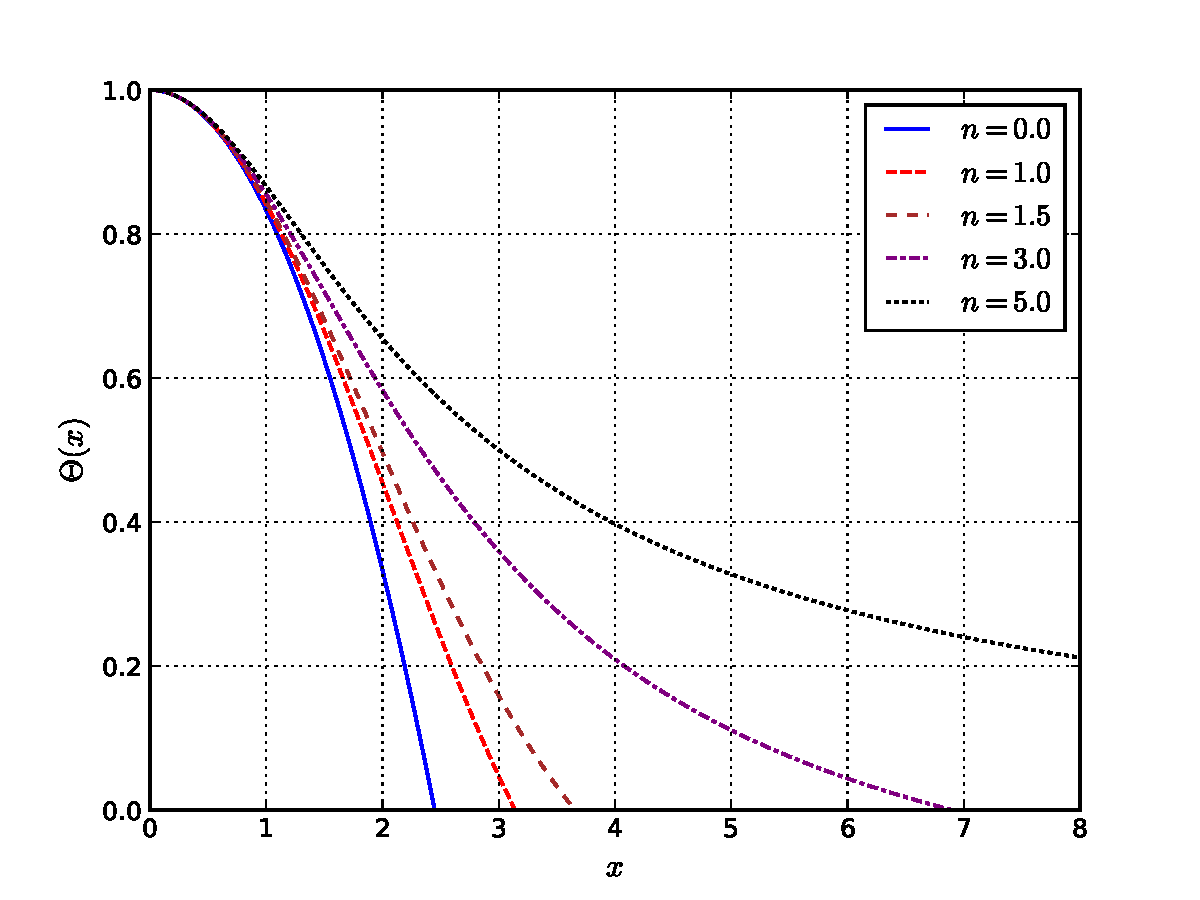
\includegraphics[angle=0,width=0.8\textwidth]{fig/fig-Lane-Emden.pdf}
\caption{Algunas soluciones de la ecuaci'on de Lane-Emden, con $n=1/(\gamma-1)$. C'odigo Python \href{https://github.com/gfrubi/GR/blob/master/figuras-editables/fig-Lane_Emden.py}{aqu\'i} (G. Neumann).}
\label{graficolane-emden}
\end{figure}

En la tabla \ref{tablalaneemden} se resumen los valores\footnote{Estos valores fueron calculados por el algoritmo de integraci'on usado y corresponden con todos los decimales (a excepci'on del 'ultimo, que puede atribuirse a la aproximaci'on o truncamiento utilizado) a los valores dados en el texto de Weinberg \cite{Weinberg72}.} de las ra'ices $x_1$ de la funci'on de Lane-Emden $\Theta(x)$, adem'as de las cantidades caracter'isticas $x_1^2\left|\Theta'(x_1)\right|$, para distintos valores del 'indice $\gamma$ 'o $n$. Estos son los valores que se usar'an en todas las secciones posteriores que los requieran para la obtenci'on de propiedades f'isicas estelares.

\begin{table}[H]
\begin{center}
\caption{Tabla de Ra'ices de la ecuaci'on de Lane-Emden}\label{tablalaneemden}
\vspace{2mm}
\begin{tabular}{|c|c|c|c|}\hline
$n$&$\gamma$ &$x_1$&$x_1^2\left|\Theta'(x_1)\right|$\\ \hline
5&6/5&$\infty$&1.73205\\
9/2&11/9&31.83646&1.73780\\
4&5/4&14.97155&1.79723\\
7/2&9/7&9.53581&1.89056\\
3&4/3&6.89685&2.01824\\
5/2&7/5&5.35528&2.187(20)\\
2&3/2&4.35287&2.41105\\
3/2&5/3&3.65375&2.71406\\
1&2&$\pi$&$\pi$\\
1/2&3&2.75280&3.78710\\
0&$\infty$&$\sqrt{6}$&2$\sqrt{6}$\\ \hline
\end{tabular}
\end{center}
\end{table}


\subsection{Comportamiento f'isico de algunas soluciones particulares}\label{sec:casos-lane-emden}

De las ecuaciones anteriores para la masa y radio de las estrellas surgen varias consecuencias importantes para el comportamiento de un modelo estelar politr'opico con determinados valores del 'indice politr'opico $\gamma$ 'o $n$, los que se detallar'an a continuaci'on:

\begin{itemize}

\item Para $\gamma\to\infty$ 'o $n=0$, que corresponde a materia incompresible, la soluci'on encontrada anal'iticamente $\Theta_0(x)$ en \eqref{lane0} coincide con la encontrada expl'icitamente en \eqref{presionnewton}, luego de retornar a las variables f'isicas por medio de las transformaciones \eqref{theta} y \eqref{x}. En efecto, considerando adem'as la ecuaci'on de estado \eqref{estadopolitropica}, \eqref{lane0} equivale a (sin consider a'un el l'imite $\gamma\to\infty$):
\begin{align}
 \left(\frac{\rho}{\rho_{\rm c}}\right)^{\gamma-1}=\left(\left(\frac{P}{P_0}\right)^{1/\gamma}\right)^{\gamma-1}&=1-\frac{1}{6}\left(\frac{4\pi G}{K}\left(1-\frac{1}{\gamma}\right)\right)\rho_{\rm c}^{2-\gamma}r^2,\\
\frac{P}{P_0}\left(\frac{P}{P_0}\right)^{1/\gamma}&=1-\frac{1}{6}\left(4\pi G\left(1-\frac{1}{\gamma}\right)\right)\frac{1}{K}\rho_{\rm c}^{2-\gamma}r^2,\\
P\left(\frac{P}{P_0}\right)^{1/\gamma}&=P_0-\frac{2}{3}\pi G\left(1-\frac{1}{\gamma}\right)\cancelto{1}{\frac{P_0}{K\rho_{\rm c}^{\gamma}}}\rho_{\rm c}^{2}r^2,
\end{align}
en donde se ha usado nuevamente \eqref{estadopolitropica} para simplificar el factor del lado derecho. Ahora,  para $\gamma\to\infty$, tendremos que $1/\gamma\to 0 $, por lo que $(P/P_0)^{1/\gamma}\to 1$ y as'i recuperamos la ecuaci'on \eqref{presionnewton} que corresponde al caso analizado de materia incompresible:
\begin{equation}
 P(r)=P_0-\frac{2}{3}\pi G\rho^2r^2
\end{equation}


Por otra parte, el hecho que la ra'iz $x_1$ sea la menor de todas las funciones $\Theta_n(x)$ para un $n$ dado, implica f'isicamente que una estrella compuesta de materia incompresible ($n=0$) es la que posee el menor radio de entre todas las estrellas politr'opicas con la misma presi'on ('o densidad) central. Este radio estar'a dado por la expresi'on general \eqref{radiopolitropico} y la ecuaci'on de estado \eqref{estadopolitropica}:
\begin{align}
 R&=\lim_{\gamma\to\infty}\left(\frac{K\gamma}{4\pi G(\gamma-1)}\right)^{1/2}\rho_{\rm c}^{\frac{\gamma}{2}-1}x_1\\
 &=\left(\frac{1}{4\pi G}\right)^{1/2}\frac{x_1}{\rho_{\rm c}}\lim_{\gamma\to\infty}\cancelto{1}{\left(\frac{\gamma}{\gamma-1}\right)^{1/2}}(K\rho_{\rm c}^\gamma)^{1/2}\\
 &=\left(\frac{1}{4\pi G}\right)^{1/2}\frac{P_0^{1/2}}{\rho_{\rm c}}x_1.
\end{align}
Pero, como $x_1=\sqrt{6}$, tendremos que el radio ser'a conocido s'olo si se especifica la raz'on $P_0/\rho_{\rm c}^2$, ya que 'este puede expresarse como:
\begin{equation}\label{rlane0}
 R=\sqrt{\frac{3}{2\pi G}\frac{P_0}{\rho_{\rm c}^2}}.
\end{equation}
% Esto puede entenderse de la manera siguiente: Si la ecuaci'on de estado politr'opica \eqref{estadopolitropica} es v'alida con $\gamma$ finito, entonces el radio $R$ ser'a expresable (por \eqref{radiopolitropico}) como funci'on de $R=R(\gamma,K,\rho_{\rm c})$. Pero en este caso, no existe un $K$ definido, por lo que se requiere expresar el radio en funci'on de otra variable, como lo es la presi'on central en la estrella, de modo tal que $R=R(\gamma,P_0,\rho_{\rm c})=R(\gamma,P_0/\rho_{\rm c}^2)=R(P_0/\rho_{\rm c}^2)$.
Cabe destacar que la relaci'on \eqref{rlane0} tambi'en puede obtenerse imponiendo la condici'on que $P(R)=0$ sobre la ecuaci'on \eqref{presionnewton}, conduciendo al mismo resultado antes hallado \eqref{ctep}.

Finalmente, la masa y la relaci'on masa-radio para este caso de materia incompresible, puede obtenerse f'acilmente, en vez de usar las ecuaciones \eqref{masalaneemden} y \eqref{masaradiopolitropico}, mediante la definici'on de densidad y la relaci'on antes hallada \eqref{rlane0}:
\begin{align}
 M=\rho V&=\frac{4}{3}\pi R^3 \rho_{\rm c}\\
 &=\frac{4}{3}\pi\rho_{\rm c} \left[\frac{3}{2\pi G}\frac{P_0}{\rho_{\rm c}^2}\right]^{3/2}\\
 &=\sqrt{\frac{6}{\pi}}\rho_{\rm c} \left(\frac{P_0}{\rho_{\rm c}^2}\right)^{3/2}.
\end{align}


\item Para $\gamma=2$ 'o $n=1$, se obtuvo la soluci'on anal'itica $\Theta_1(x)$ en \eqref{lane1}, cuya primera ra'iz es $x_1=\pi$. Reemplazando en el radio de la estrella \eqref{radiopolitropico}, se observa de inmediato que 'este ser'a independiente de la densidad central, pues
 \begin{equation}
  R=\left(\frac{2K}{4\pi G(2-1)}\right)^{1/2}\rho_{\rm c}^{\frac{2}{2}-1}\pi.
 \end{equation}
As'i, tendremos el radio para una estrella politr'opica con $\gamma=2$:
\begin{equation}
 R=\sqrt{\frac{\pi K}{2G}},
\end{equation}
que depende 'unicamente de la constante $K$ de la ecuaci'on de estado politr'opica.

\item  Para $\gamma=6/5$ 'o $n=5$, tambi'en se obtuvo una soluci'on anal'itica $\Theta_5(x)$ en \eqref{lane5}, en donde la primera ra'iz s'olo se alcanza en $x_1\to\infty$. Por \eqref{radiopolitropico}, una estrella con este 'indice adiab'atico tendr'ia un radio infinito, para cualquier valor finito de la densidad central $\rho_{\rm c}$. Por otra parte, la masa de estas estrellas estar'ia dada por \eqref{masalaneemden}, tomando el l'imite cuando $x_1\to\infty$:
\begin{align}
 M=4\pi\rho_{\rm c}^{\frac{3\cdot6/5-4}{2}}\left(\frac{K\cdot6/5}{4\pi G(6/5-1)}\right)^{3/2}\lim_{x_1\to\infty}x_1^2\left|\Theta'_5(x_1)\right|.
\end{align}
El l'imite anterior se puede calcular en base a \eqref{lane5}:
\begin{align}
 \lim_{x_1\to\infty}x_1^2\left|\Theta'_5(x_1)\right|&=\lim_{x_1\to\infty}x_1^2\left|\frac{d}{dx}\left.\left(\frac{1}{1+\frac{x^2}{3}}\right)^{1/2}\right|_{x=x_1}\right|\\
 &=\lim_{x_1\to\infty}\frac{1}{3}\frac{x_1^3}{\left(1+\frac{x_1^2}{3}\right)^{3/2}}\\
 &=\lim_{x_1\to\infty}3^{1/2}\frac{1}{\left(\frac{3}{x_1^2}+1\right)^{3/2}}\\
 &=\sqrt{3}
\end{align}
De esta forma, podemos ver que la masa de una estrella con $\gamma=6/5$ es finita, aunque su radio sea infinito, estando dada por:
\begin{equation}
 M=36\pi\left(\frac{K}{4\pi G}\right)^{3/2}\rho_{\rm c}^{-1/5}.
\end{equation}


 \item De la ecuaci'on de masa \eqref{masalaneemden} 'o \eqref{lane-masagamma}, se puede ver que la masa de la estrella $M$ es creciente con respecto su densidad central $\rho_{\rm c}$ para $\gamma>4/3$ ($n<3$), mientras que para $\gamma<4/3$ ($n>3$) es decreciente. De forma an'aloga, considerando ahora la relaci'on masa-radio \eqref{masaradiopolitropico}, podemos ver que el mismo comportamiento existe con respecto al radio: la masa de la estrella $M$ es creciente con respecto a su radio $R$ para $\gamma>4/3$ ($n<3$), mientras que para $\gamma<4/3$ ($n>3$) es decreciente. Estos hechos tienen importantes consecuencias para la estabilidad estelar.

 \item Para $\gamma=4/3$ 'o $n=3$, de acuerdo a la discusi'on del 'item anterior, la masa de la estrella ser'a independiente de la densidad central y del radio, estando dada por \eqref{masalaneemden}:
\begin{align}\label{masa4/3}
 M=4\pi\left(\frac{K}{\pi G}\right)^{3/2}x_1^2\left|\Theta'(x_1)\right|
 =4\cdot2.01824\cdot\pi\left(\frac{K}{\pi G}\right)^{3/2}=:M_{\rm ch},
\end{align}
en donde se ha usado el valor de $x_1^2\left|\Theta'(x_1)\right|$ obtenido num'ericamente de la funci'on de Lane-Emden $\Theta_3(x)$, recopilado en la tabla \ref{tablalaneemden}. Esta cantidad se denomina \emph{Masa de Chandrasekhar} $M_{\rm ch}$, y representa un valor l'imite que posee una importante interpretaci'on f'isica para ciertos tipos de estrellas, como se mostrar'a posteriormente.
 Por completitud, tambi'en se dar'a la expresi'on expl'icita para el radio asociado a este 'indice politr'opico usando \eqref{radiopolitropico}, aunque m'as adelante se ver'a que esta aproximaci'on carece de valor pr'actico.
\begin{align}\label{radio4/3}
 R=\left(\frac{K}{\pi G}\right)^{1/2}\rho_{\rm c}^{-1/3}x_1
 =6.89685\left(\frac{K}{\pi G}\right)^{1/2}\rho_{\rm c}^{-1/3},
\end{align}
en donde se ha usado el valor de $x_1$ hallado en la tabla \ref{tablalaneemden}.

\item Para $\gamma=5/3$ 'o $n=3/2$, que corresponde al 'indice politr'opico de un gas ideal (ver justificaci'on en el ap'endice \ref{cap:termo}), podemos ver que su radio se obtiene de \eqref{radiopolitropico} simplemente reemplazando este valor y usando los valores de $x_1$ de la tabla \ref{tablalaneemden}:
\begin{equation}\label{radio5/3}
 R=\left(\frac{5K}{8\pi G}\right)^{1/2}\rho_{\rm c}^{-1/6}x_1=3.65375\left(\frac{5K}{8\pi G}\right)^{1/2}\rho_{\rm c}^{-1/6}.
\end{equation}
As'i mismo, podemos encontrar una expresi'on para la masa a partir de \eqref{masalaneemden} y de la tabla \ref{tablalaneemden}:
\begin{equation}\label{masa5/3}
 M=4\pi\rho_{\rm c}^{1/2}\left(\frac{5K}{8\pi G}\right)^{3/2}x_1^2\left|\Theta'(x_1)\right|=4\cdot2.71406\cdot\pi\rho_{\rm c}^{1/2}\left(\frac{5K}{8\pi G}\right)^{3/2}.
\end{equation}
Finalmente, usando la ecuaci'on masa-radio \eqref{masaradiopolitropico}, podemos ver que:
\begin{align}
M&=4\pi R^{-3}\left(\frac{5K}{8\pi G}\right)^3x_1^3\left\{x_1^2\left|\Theta'(x_1)\right|\right\}\label{masaradio5/3},\\
\Rightarrow\quad M\left[\frac{4\pi}{3}R^3\right]&=\frac{1}{3}\frac{1}{4\pi}\left(\frac{5K}{2G}\right)x_1^3\left\{x_1^2\left|\Theta'(x_1)\right|\right\}.
\end{align}
Identificando el factor en par'entesis cuadrado en el lado izquierdo de la igualdad anterior como el volumen $V$ de la estrella, encontramos que el producto de la masa y volumen para este modelo estelar es constante, estando dado por
\begin{equation}
 MV=\frac{1}{3\cdot 2^5\pi}\left(\frac{5K}{G}\right)^3 x_1^ 3\left\{x_1^2\left|\Theta'(x_1)\right|\right\}=\frac{132.384}{3\cdot 2^5\pi}\left(\frac{5K}{G}\right)^3\label{masavolumen5/3}.
\end{equation}

\end{itemize}


\subsubsection{Determinaci'on de par'ametros estelares en funci'on de \texorpdfstring{$M$}{M}, \texorpdfstring{$R$}{R} y \texorpdfstring{$\gamma$}{gamma}}

Para poder constrastar los resultados obtenidos mediante el modelo estelar newtoniano descrito, con respecto a las cantidades f'isicas directamente provistas por las observaciones, se requiere reescribir las relaciones anteriores y sus soluciones de la forma detallada a continuaci'on. Se supondr'a que los par'ametros conocidos de una estrella son su \emph{masa} $M$, su \emph{radio} $R$ y el \emph{'indice politr'opico} $\gamma$ del gas que la compone. Luego, el procedimiento para modelar dicha estrella ser'a:

\begin{enumerate}
 \item Como $\gamma$ es dado, $n$ ser'a conocido mediante \eqref{ngamma}. As'i, por cada $n\in[0,5]$, la ecuaci'on de Lane-Emden \eqref{laneemden} tendr'a una soluci'on 'unica $\Theta_n(x)$, que en general se encuentra num'ericamente. El conocimiento de la funci'on de Lane-Emden anterior tambi'en proporciona su primera ra'iz positiva $x_1$ (en donde $\Theta(x_1)=0$), y adem'as $x_1^2\left|\Theta'(x_1)\right|$.
\item La constante $K$ de la ecuaci'on de estado politr'opica \eqref{estadopolitropica} queda completamente determinada. En efecto, de la relaci'on \eqref{masaradiopolitropico}, escrita en t'erminos de $n$, es posible despejar $K$ en t'erminos de las cantidades conocidas $M$, $R$, $x_1$ y $x_1^2\left|\Theta'(x_1)\right|$:
\begin{align}
M&=4\pi R^{\frac{n-3}{n-1}}\left(\frac{K(1+n)}{4\pi G}\right)^{\frac{n}{n-1}}x_1^{-\frac{n-3}{n-1}}\,x_1^2\left|\Theta'(x_1)\right|,\\
% M^{\frac{n-1}{n}}&=(4\pi)^{\frac{n-1}{n}}R^{\frac{n-3}{n}}\frac{K}{4\pi G}(1+n)x_1^{\frac{n+1}{n-1}\frac{n-1}{n}}\left|\Theta'(x_1)\right|^{\frac{n-1}{n}}\\
% GM^{\frac{n-1}{n}}R^{\frac{3-n}{n}}&=K\frac{(n+1)}{(4\pi)^{1/n}}x_1^{\frac{n+1}{n}}\left|\Theta'(x_1)\right|^{\frac{n-1}{n}}\\
% \Rightarrow\quad K&=\frac{1}{n+1}\left(\frac{4\pi}{x_1^{n+1}\left|\Theta'(x_1)\right|^{n-1}}\right)^{1/n}GM^{\frac{n-1}{n}}R^{\frac{3-n}{n}}
% \end{align}
% De esta forma, tendremos finalmente que:
% \begin{equation}
\Rightarrow\quad K&=\frac{1}{n+1}\left(\frac{4\pi}{x_1^{3-n} \left(x_1^2\left|\Theta'(x_1)\right|\right)^{n-1}}\right)^{1/n}GM^{1-\frac{1}{n}}R^{\frac{3}{n}-1}.\label{kpolitropico}
\end{align}

 \item La densidad central $\rho_{\rm c}$ presente en la normalizaci'on que condujo a la definici'on de la variable $\Theta(x)$, ya se determin'o en t'erminos de las variables conocidas en \eqref{densidad0politropica}.
% en se puede obtener f'acilmente reemplazando el resultado anterior \eqref{kpolitropico} en \eqref{radiopolitropico} (escrita en t'erminos de $n$):
% \begin{align}
% R&=\left(\frac{K(1+n)}{4\pi G}\right)^{1/2}\rho_{\rm c}^{\frac{1-n}{2n}}x_1\\
% R^{\frac{2n}{1-n}}&=\left(\frac{K(1+n)}{4\pi G}\right)^{\frac{n}{1-n}}x_1^{\frac{2n}{1-n}}\rho_{\rm c}\\
% R^{\frac{2n}{1-n}}&=\left(\frac{1+n}{4\pi G}\right)^{\frac{n}{1-n}}\left[\frac{1}{n+1}\left(\frac{4\pi}{x_1^{3-n} \left(x_1^2\left|\Theta'(x_1)\right|\right)^{n-1}}\right)^{\frac{1}{n}}GM^{1-\frac{1}{n}}R^{\frac{3}{n}-1}\right]^{\frac{n}{1-n}}x_1^{\frac{2n}{1-n}}\rho_{\rm c}\\
% R^{\frac{2n}{1-n}}&=4\pi\frac{x_1^2\left|\Theta'(x_1)\right|}{x_1^3}\frac{R^{\frac{3-n}{1-n}}}{M}\rho_{\rm c}
% \end{align}
% Es decir, obtenemos la densidad central en t'erminos de cantidades conocidas:

\item La densidad $\rho(r)$ entonces queda completamente determinada al expresarla en funci'on de la funci'on de Lane-Emden $\Theta(x)$ por medio de \eqref{theta}, pues usando $\rho_{\rm c}$ dado en \eqref{densidad0politropica} podemos escribir:
\begin{align}
 \rho(r)&=\rho_{\rm c}\left[\Theta(x)\right]^n\label{rhoder}\\
&=\frac{1}{4\pi}\frac{x_1^3}{x_1^2\left|\Theta'(x_1)\right|}\frac{M}{R^3}\left[\Theta(x)\right]^n,
\end{align}
y considerando \eqref{laneemden-rax}:
\begin{equation}\label{densidadpolitropica}
 \rho(r)=\frac{1}{4\pi}\frac{x_1^3}{x_1^2\left|\Theta'(x_1)\right|}\frac{M}{R^3}\left[\Theta\left(x_1\frac{r}{R}\right)\right]^n.
\end{equation}

\item Usando la ecuaci'on de estado \eqref{estadopolitropica}, podemos determinar directamente tambi'en la presi'on en el centro de la estrella $P_0$, pues eval'uandola all'i:
\begin{equation}
 P_0=K\rho_{\rm c}^{1+\frac{1}{n}}.
\end{equation}
As'i, reemplazando \eqref{kpolitropico} y \eqref{densidad0politropica}, tenemos:
\begin{align}
%  P_0&=\frac{1}{n+1}\left(\frac{4\pi}{x_1^{3-n} \left(x_1^2\left|\Theta'(x_1)\right|\right)^{n-1}}\right)^{1/n}GM^{1-\frac{1}{n}}R^{\frac{3}{n}-1}\left[\frac{1}{4\pi}\frac{x_1^3}{x_1^2\left|\Theta'(x_1)\right|}\frac{M}{R^3}\right]^{1+\frac{1}{n}}\\
P_0&=\frac{1}{4\pi(n+1)}\frac{x_1^4}{\left(x_1^2\left|\Theta'(x_1)\right|\right)^2}\frac{GM^2}{R^4}\label{presionpolitropica}.
\end{align}
\item An'alogamente, tambi'en podemos determinar la dependencia radial de la presi'on al interior de la estrella, usando \eqref{estadopolitropica} y \eqref{rhoder}:
\begin{align}
 P(r)=K\rho(r)^{1+\frac{1}{n}}=K\left(\rho_{\rm c}\left[\Theta(x)\right]^n\right)^{1+\frac{1}{n}}=P_0\left[\Theta(x)\right]^{1+n}.
\end{align}
Entonces, reemplazando \eqref{presionpolitropica}, tenemos que la forma expl'icita del perfil de presi'on en la estrella vendr'a dado por:
\begin{equation}
 P(r)=\frac{1}{4\pi(n+1)}\frac{x_1^4}{\left(x_1^2\left|\Theta'(x_1)\right|\right)^2}\frac{GM^2}{R^4}\left[\Theta\left( x_1\frac{r}{R}\right)\right]^{1+n}.
\end{equation}






\end{enumerate}

\section{Soluci'on exacta para gas de Fermi}\label{sec:fermi-exacta}

Un caso mucho m'as realista que los tratados anteriormente para resolver el sistema de ecuaciones de estructura estelar, es considerar la ecuaci'on de estado exacta de un gas de Fermi completamente degenerado (a $T=0$), dada en forma impl'icita por las ecuaciones \eqref{presionfermi2} y \eqref{densidad_electrones-fermi}, que se pueden expresar respectivamente como:
\begin{align}\label{ec-estado-fermi}
 P&=Af(x),&\rho&=Bx^3,
\end{align}
en donde $x$ es un par'ametro adimensional expresado en funci'on del momentum de Fermi por \eqref{xrelativo}, en t'erminos del cual se define:
\begin{equation}\label{ec-fermi-fx}
 f(x)=x\sqrt{1+x^2}\left(2x^2-3\right)+3\senh^{-1}x.
\end{equation}
Adem'as, $A$ es una constante dada por:
\begin{align}\label{ec-fermi-A}
 A_{e,n}&=\frac{\pi m_{e,n}^4 c^5}{3 h^3},
\end{align}
tanto para electrones ($e$) como neutrones ($n$), mientras que $B$ es otra constante que para electrones y neutrones toma respectivamente los valores:
\begin{align}\label{ec-fermi-B}
B_e=\frac{8\pi m_e^3 c^3}{3h^3}m_u\mu_e,\qquad\qquad B_n=\frac{8\pi m_n^4 c^3}{3h^3}&
\end{align}

\subsection{Ecuaci'on de estructura de Fermi}
En principio tenemos las tres inc'ognitas, $P$, $\rho$ y $M$, por determinar, la 'ultima de las cuales se puede despejar siguiendo el procedimiento que condujo a la ecuaci'on diferencial \eqref{eq-hidrostatico-sinm} de $P$ y $\rho$ en funci'on de la coordenada radial $r$. Sustituyendo la ecuaci'on de estado \eqref{ec-estado-fermi}, tenemos:
\begin{align}
\frac{1}{Br^2}\frac{d}{dr}\left(\frac{r^2}{x^3}\frac{dP}{dx}\frac{dx}{dr}\right)&=-4\pi G B x^3.
\end{align}
Notando que la derivada de la presi'on con respecto a $x$ se puede determinar directamente del integrando de \eqref{presionfermi1}, obtenemos:
\begin{align}
\frac{1}{Br^2}\frac{d}{dr}\left(\frac{r^2}{x^3}\frac{8Ax^4}{\sqrt{1+x^2}}\frac{dx}{dr}\right)&=-4\pi G B x^3,\\
\frac{1}{r^2}\frac{d}{dr}\left(r^2\frac{x}{\sqrt{1+x^2}}\frac{dx}{dr}\right)&=-\frac{\pi G B^2}{2A} x^3,\\
\frac{1}{r^2}\frac{d}{dr}\left(r^2\frac{d}{dr}\sqrt{1+x^2}\right)&=-\frac{\pi G B^2}{2A} x^3.
\end{align}
Haciendo la sustituci'on:
\begin{align}\label{sust-fermi}
 y:=\sqrt{1+x^2},\qquad\Rightarrow\qquad x=\sqrt{y^2-1},
\end{align}
tenemos que:
\begin{align}\label{ec-fermi1}
\frac{1}{r^2}\frac{d}{dr}\left(r^2\frac{dy}{dr}\right)&=-\frac{\pi G B^2}{2A} \left(y^2-1\right)^{3/2},
\end{align}
ecuaci'on an'aloga a la de Lane-Emden \eqref{laneemden}, por lo que podemos usar t'ecnicas similares para encontrar sus soluciones. En primer lugar, se escribe en t'erminos de la coordenada radial adimensional $\eta$ y de la variable reescalada $\phi$, definidas por:
\begin{equation}\label{cambio-fermi-adim}
 r=a\eta,\qquad\text{y}\qquad y=y_0\phi,
\end{equation}
con $y_0$ constante, reminiscente de la densidad central de la estrella $\rho_{\rm c}$ (comparar con el cambio de variables de Lane-Emden \eqref{x} y \eqref{theta}). Para encontrar $a$, reemplazamos en \eqref{ec-fermi1}:
\begin{align}
\frac{1}{(a\eta)^2}\frac{d}{d(a\eta)}\left((a\eta)^2\frac{d(y_0\phi)}{d(a\eta)}\right)&=-\frac{\pi G B^2}{2A} \left((y_0\phi)^2-1\right)^{3/2},\\
\frac{1}{\eta^2}\frac{d}{d\eta}\left(\eta^2\frac{d\phi}{d\eta}\right)&=-a^2\frac{\pi G B^2 y_0^2}{2A}\left(\phi^2-\frac{1}{y_0^2}\right)^{3/2}.
\end{align}
As'i, definiendo:
\begin{equation}\label{ec-fermi-a}
 a:=\sqrt{\frac{2A}{\pi G}}\frac{1}{B y_0}=\frac{l}{y_0},
\end{equation}
con $l$ una escala de longitud independiente de $y_0$, obtenemos \emph{la ecuaci'on de estructura de Fermi}, dependiente del par'ametro $y_0$ (comparar con \eqref{laneemden} que depende, en cambio, del par'ametro $n$ 'o $\gamma$):
\begin{align}\label{ec-fermi2}
\boxed{
\frac{1}{\eta^2}\frac{d}{d\eta}\left(\eta^2\frac{d\phi}{d\eta}\right)=-\left(\phi^2-\frac{1}{y_0^2}\right)^{3/2}.}
\end{align}
Las condiciones de borde son las mismas de Lane-Emden para la variable $\Theta$, ya que en el centro de la estrella $y(\eta=0)=y_0$, y as'i:
\begin{equation}\label{bcs-fermi}
\phi(\eta=0)=1\qquad\text{y}\qquad \phi'(\eta=0)=0,
\end{equation}
en donde la segunda condici'on se justifica de la misma forma que en \eqref{divergencia2}.

\subsection{Propiedades f'isicas de la ecuaci'on de estructura de Fermi}

\subsubsection{Radio de la estrella}
Al igual que en el caso de la ecuaci'on de Lane-Emden, tenemos que las soluciones $\phi=\phi(\eta)$ son mon'otonamente decrecientes. Como dicha variable est'a relacionada con $y$  de acuerdo a \eqref{cambio-fermi-adim}, 'esta a su vez con $x$ a trav'es de \eqref{sust-fermi}, que a su vez es parte de la ecuaci'on de estado para la densidad $\rho$ \eqref{ec-estado-fermi}, vemos que:
\begin{equation}\label{rho-x-y-phi}
\begin{split}
 \rho=Bx^3=B\left(y^2-1\right)^{3/2}&=B\left[(y_0\phi)^2-1\right]^{3/2}\\
&=By_0^3\left(\phi^2-\frac{1}{y_0^2}\right)^{3/2}.
\end{split}
\end{equation}
Luego, es claro que la densidad tambi'en ser'a mon'otonamente decreciente. Por lo tanto, se definir'a el radio de la estrella, al igual que para Lane-Emden, como aquella coordenada radial adimensional $\eta_1$ en que la densidad se anule: $\rho(\eta_1)=0$. Como de la ecuaci'on anterior esto equivale a que $x(\eta_1)=0$, vemos de \eqref{ec-estado-fermi} y \eqref{ec-fermi-fx} que la presi'on de la estrella tambi'en se anular'a all'i: $P(x=0)=0$, lo cual es consistente con lo que uno esperar'ia f'isicamente para el borde de una estrella. Ahora bien, esta condici'on implica, por \eqref{rho-x-y-phi}, que:
\begin{equation}
%  0=\rho(\eta_1)=B\left((y_0\phi(\eta_1))^2-1\right)^{3/2}\quad\Rightarrow\quad
\phi(\eta_1)=\frac{1}{y_0}\label{ec-fermi-raices}
\end{equation}
Consistentemente, tendremos de la definici'on de la variable $\eta$ en \eqref{cambio-fermi-adim}, que el radio f'isico $R$ de la estrella vendr'a dado, al considerar \eqref{ec-fermi-a}, por:
\begin{equation}\label{ec-fermi-radio}
\boxed{
\begin{aligned}
 R&=a\eta_1=l\frac{\eta_1}{y_0}\\
&=\sqrt{\frac{2A}{\pi G}}\frac{1}{B}\frac{\eta_1}{y_0}.
\end{aligned}}
\end{equation}

Al igual que para el caso de Lane-Emden, el radio adimensional $\eta_1$ se obtiene, para cada $y_0$, resolviendo la ecuaci'on de estructura de Fermi mediante m'etodos num'ericos, que se describir'an en la secci'on \ref{sec:fermi-numerico}.

\subsubsection{Masa de la estrella}

La masa de la estrella al interior del radio adimensional $\eta$ se obtendr'a a partir de su definici'on en \eqref{masa1} y de \eqref{ec-fermi-dens}:
\begin{align}
 \mathcal{M}(\eta)&=4\pi\int\limits^R_{0}dr'r'^2\rho(r')=4\pi a^3\int\limits^{\eta}_{0}d\eta' \eta'^2\rho\\
&=4\pi B y_0^3 a^3\int\limits^{\eta}_{0} \left(\phi^2-\frac{1}{y_0^2}\right)^{3/2}\eta'^2d\eta'.
\end{align}
Pero, al igual que para Lane-Emden, notamos que de la ecuaci'on de estructura de Fermi  \eqref{ec-fermi2}:
\begin{align}
 \eta^2\left(\phi^2-\frac{1}{y_0^2}\right)^{3/2}&=-\frac{d}{d\eta}\left(\eta^2\frac{d\phi}{d\eta}\right),\\
\Rightarrow\quad \int\limits^{\eta}_{0} \left(\phi^2-\frac{1}{y_0^2}\right)^{3/2}\eta'^2d\eta'&=\eta^2\left\Vert\phi'(\eta)\right\Vert,
\end{align}
en donde se toma el valor absoluto puesto que $\phi'(\eta)<0$ (soluciones decrecientes). Luego, la masa al interior de $\eta$ se podr'a expresar usando tambi'en la definici'on de $a$ en \eqref{ec-fermi-a}, como:
\begin{align}
\mathcal{M}(\eta)&=4\pi B y_0^3 a^3\eta^2\left\Vert\phi'(\eta)\right\Vert\label{ec-fermi-masaparcial1}\\
&=4\pi\left(\frac{2A}{\pi G}\right)^{3/2}\frac{1}{B^2}\,\eta^2\left\Vert\phi'(\eta)\right\Vert\label{ec-fermi-masaparcial2}.
\end{align}
La masa total  de la estrella ser'a toda aquella al interior de su radio adimensional $M:=\mathcal{M}(\eta_1)$, por lo que evaluando la expresi'on anterior en $\eta_1$, encontramos:
\begin{equation}\label{ec-fermi-masatotal}
\boxed{
 M=4\pi\left(\frac{2A}{\pi G}\right)^{3/2}\frac{1}{B^2}\eta_1^2\left\Vert\phi'(\eta_1)\right\Vert.}
\end{equation}
Note que aqu'i el par'ametro $y_0$ de la ecuaci'on de estructura s'olo aparece impl'icitamente, a trav'es de la soluci'on $\phi$ y la cantidad caracter'istica $\eta_1^2\left\Vert\phi'(\eta_1)\right\Vert$, que se encuentran num'ericamente (ver secci'on \eqref{sec:fermi-numerico}).

\subsubsection{Densidad central y media}
La densidad central de la estrella $\rho_{\rm c}$ se conseguir'a evaluando \eqref{rho-x-y-phi} en $\eta=0$ y aplicando la condici'on de borde \eqref{bcs-fermi}:
\begin{align}
 \rho_{\rm c}:&=\rho(\eta=0)=B\left[(y_0\phi(\eta=0))^2-1\right]^{3/2}\\
&=B\left(y_0^2-1\right)^{3/2}=By_0^3\left(1-\frac{1}{y_0^2}\right)^{3/2}.\label{ec-fermi-byrho1}
\end{align}
De esta forma, tendremos que la densidad central es funci'on 'unicamente del par'ametro $y_0$ de la ecuaci'on de estructura de Fermi:
\begin{equation}\label{ec-fermi-byrho2}
 \boxed{\rho_{\rm c}=B(y_0^2-1)^{3/2}}
\end{equation}

Por otra parte, el perfil de densidad de la estrella se puede expresar reescribiendo \eqref{rho-x-y-phi} y usando la relaci'on anterior:
\begin{align}
 \rho(r)&=By_0^3\left(\phi(\eta)^2-\frac{1}{y_0^2}\right)^{3/2}\label{ec-fermi-dens}\\
&=\rho_{\rm c}\frac{y_0^3}{\left(y_0^2-1\right)^{3/2}}\left(\phi(\eta)^2-\frac{1}{y_0^2}\right)^{3/2}\\
&=\rho_{\rm c}\left(\frac{\phi(\eta)^2-\frac{1}{y_0^2}}{1-\frac{1}{y_0^2}}\right)^{3/2}.
\end{align}
Tambi'en podemos establecer una relaci'on similar a la de Lane-Emden entre la densidad media $\bar{\rho}$ y la densidad central $\rho_{\rm c}$ de la estrella. Para ello, notamos que la densidad media de materia dentro del radio $\eta$ se expresar'a en funci'on de la masa al interior de dicho radio por medio de \eqref{ec-fermi-masaparcial1}:
\begin{align}
 \bar{\rho}(\eta)&=\frac{\mathcal{M}(r)}{\frac{4}{3}\pi r^3},\\
&=\frac{\cancel{4\pi} B y_0^3 \cancel{a^3}\eta^2\left\Vert\phi'(\eta)\right\Vert}{\frac{\cancel{4}}{3}\cancel{\pi} (\cancel{a}\eta)^3},
\end{align}
y expresando $B$ en t'erminos de $\rho_{\rm c}$ por medio de \eqref{ec-fermi-byrho1}, tendremos la siguiente relaci'on entre la densidad media parcial y la central\footnote{Consistemente, es f'acilmente verificable, a partir de la relaci'on mostrada, que $\lim_{\eta\to 0}\bar{\rho}(\eta)=\rho_{\rm c}$. En efecto, usando la regla de L'H\^opital y recordando la condici'on de borde $\phi'(0)=0$, vemos que:
\begin{align}
\lim_{\eta\to 0}\bar{\rho}=\frac{3\rho_{\rm c}}{\left(1-\frac{1}{y_0^2}\right)^{3/2}}\lim_{\eta\to 0}\frac{\left\Vert\phi'(\eta)\right\Vert}{\eta}
=
\frac{3\rho_{\rm c}}{\left(1-\frac{1}{y_0^2}\right)^{3/2}}\lim_{\eta\to 0}\frac{\left\Vert\phi''(\eta)\right\Vert}{1}\label{ec-fermi-limite-rho}
\end{align}
Luego, despejando $\phi''(\eta)$ de la ecuaci'on de estructura \eqref{ec-fermi2} (lo que se har'a expl'icitamente en \eqref{ec-fermi-phi''}), podemos reemplazarlo en el l'imite anterior y recordando la condici'on de borde $\phi(0)=0$, obtenemos la relaci'on:
\begin{align}
\lim_{\eta\to 0}\phi''(\eta)&=\lim_{\eta\to 0}\frac{\phi'(\eta)}{\eta}=\lim_{\eta\to 0}-\left[2\frac{\phi'(\eta)}{\eta}+\left(\phi(\eta)-\frac{1}{y_0^2}\right)^{3/2}\right]\\
\Rightarrow\quad\lim_{\eta\to 0}3\frac{\phi'(\eta)}{\eta}&=-\left(\phi(0)-\frac{1}{y_0^2}\right)^{3/2}\\
\Rightarrow\quad\lim_{\eta\to 0}\left\Vert\phi''(\eta)\right\Vert&=\frac{1}{3}\left(1-\frac{1}{y_0^2}\right)^{3/2}
\end{align}
As'i, reemplazando el l'imite anterior en \eqref{ec-fermi-limite-rho}, obtenemos finalmente que:
$\lim_{\eta\to 0}\bar{\rho}(\eta)=\rho_{\rm c}.$
}:
\begin{align}
\bar{\rho}(\eta)=\frac{3\rho_{\rm c}}{\left(1-\frac{1}{y_0^2}\right)^{3/2}}\frac{\eta^2\left\Vert\phi'(\eta)\right\Vert}{\eta^3},
\end{align}
y para la densidad media total $\bar{\rho}$ de la estrella, en $\eta=\eta_1$; obtenemos:
\begin{align}\label{ec-fermi-densidadmediaycentral}
\boxed{\bar{\rho}=\frac{3\rho_{\rm c}}{\left(1-\frac{1}{y_0^2}\right)^{3/2}}\frac{\eta_1^2\left\Vert\phi'(\eta_1)\right\Vert}{\eta_1^3},}
\end{align}
es decir, la densidad media ser'a proporcional a la densidad central, pues los otros factores dependen s'olo de la soluci'on a la ecuaci'on de estructura de Fermi para un $y_0$ dado (comparar con el resultado de Lane-Emden \eqref{laneemden-densidadmedia}). Y como la densidad media total de una estrella es $\bar{\rho}=M/(4\pi R^3/3)$, tendremos que la densidad central tambi'en se puede expresar en funci'on de su radio y masa total:
\begin{equation}
\boxed{ \rho_{\rm c}= \frac{1}{4\pi}\left(1-\frac{1}{y_0^2}\right)^{3/2}\frac{\eta_1^3}{\eta_1^2\left\Vert\phi'(\eta_1)\right\Vert}\frac{M}{R^3}.}
\end{equation}



\subsection{Casos l'imite de las soluciones}\label{sec:ec-fermi-limites}

\subsubsection{Aproximaci'on de bajas densidades}
De la ecuaci'on de estado de Fermi \eqref{ec-estado-fermi} para la densidad en t'erminos del par'ametro $x$ , notamos que si esta cantidad evaluada en el centro de la estrella es peque\~na: $x(\eta=0)=x_0\ll1$, entonces la densidad central de la estrella, $\rho_{\rm c}=Bx_0^3$, tambi'en lo ser'a ($\rho_{\rm c}\ll B$, en donde los valores num'ericos de esta constante est'an dados en \eqref{densidad_electrones-fermi} y \eqref{densidad_neutrones-fermi}). Por lo tanto, en la aproximaci'on de bajas densidades a analizar, se despreciar'an t'erminos de orden $\mathcal{O}(x_0^4)$, y as'i, el lado derecho de la ecuaci'on de estructura de Fermi \eqref{ec-fermi2} se podr'a escribir, al considerar \eqref{sust-fermi}, como:
\begin{align}
 -\left(\phi^2-\frac{1}{y_0^2}\right)^{3/2}&=-\left(\phi^2-\frac{1}{1+x_0^2}\right)^{3/2}\\
&\approx-\left(\phi^2-(1-x_0^2)\right)^{3/2}.
\end{align}
Definiendo
\begin{equation}\label{ec-fermi-sust-5/3-1}
 \widetilde{\Theta}:=\phi^2-(1-x_0^2),
\end{equation}
podemos expresar $\phi$ en t'erminos de $\widetilde{\Theta}$,
\begin{align}
\phi=\sqrt{1+\widetilde{\Theta}-x_0^2}\approx1-\frac{1}{2}\left(x_0^2-\widetilde{\Theta}\right)\qquad\Rightarrow\quad \frac{d\phi}{d\eta}\approx\frac{1}{2}\frac{d\widetilde{\Theta}}{d\eta},\label{ec-fermi-sust-5/3}
\end{align}
y as'i, podemos cambiar la variable dependiente en la ecuaci'on de estructura de Fermi \eqref{ec-fermi2} de $\phi$ a $\widetilde{\Theta}$:
\begin{align}\label{ec-fermi-ec5/3-1}
 \frac{1}{2}\frac{1}{\eta^2}\frac{d}{d\eta}\left(\eta^2\frac{d\widetilde{\Theta}(\eta)}{d\eta}\right)=-\left[\widetilde{\Theta}(\eta)\right]^{3/2},
\end{align}
por lo que cambiando la variable independiente a $\widetilde{x}=\sqrt{2}\eta$, tenemos:
\begin{align}\label{ec-fermi-ec5/3-2}
 \frac{1}{\widetilde{x}^2}\frac{d}{d\widetilde{x}}\left(\widetilde{x}^2\frac{d\widetilde{\Theta}(\widetilde{x})}{d\widetilde{x}}\right)=-\left[\widetilde{\Theta}(\widetilde{x})\right]^{3/2},
\end{align}
es decir, hemos recuperado la ecuaci'on de Lane-Emden  \eqref{laneemden} de 'indice $n=3/2$, pero con condiciones de borde distintas, ya que en el origen $\eta=0$, la variable $\bar{\Theta}$  definida en \eqref{ec-fermi-sust-5/3-1} tomar'a el valor:
\begin{align}\label{ec-fermi-bcs5/3}
 \widetilde{\Theta}(0)=\left(\underbrace{\cancelto{1}{\phi(0)}^2}_{\text{\eqref{bcs-fermi}}}-(1-x_0^2)\right)=x_0^2,
\end{align}
a diferencia de la funci'on de Lane-Emden $\Theta_{3/2}(x)$ que satisface $\Theta_{3/2}(x=0)=1$. Pero igualmente se puede aprovechar esta soluci'on conocida, notando que la funci'on definida por:
\begin{equation}\label{ec-fermi-thetatilde5/3}
 \widetilde{\Theta}(\widetilde{x})=x_0^2\Theta_{3/2}(\sqrt{x_0} \,\widetilde{x}),
\end{equation}
tambi'en ser'a una soluci'on de la misma ecuaci'on de Lane-Emden\footnote{Esta es una caracter'istica general de la soluciones de la ecuaci'on de Lane-Emden, denominada propiedad de \emph{homolog'ia}: Si $\Theta_n(x)$ es una soluci'on de la ecuaci'on de Lane-Emden \eqref{laneemden} de 'indice $n$ con la condici'on de borde usual $\Theta_n(0)=1$, entonces $\widetilde{\Theta}(x)=A^{\frac{2}{n-1}}\Theta_n(Ax)$ tambi'en ser'a soluci'on de la misma ecuaci'on, pero con condici'on de borde $\widetilde{\Theta}(0)=A^{\frac{2}{n-1}}$.}. En efecto, reemplazando $\widetilde{\Theta}(x)$ en el lado izquierdo de \eqref{laneemden} con $n=3/2$:
\begin{align} \frac{1}{x^2}\frac{d}{dx}\left(x^2\frac{d\widetilde{\Theta}(x)}{dx}\right)&=\frac{x_0^2}{x^2}\frac{d}{dx}\left(x^2\frac{d}{dx}\Theta_{3/2}(\sqrt{x_0}x)\right),\\
&=x_0^2(\sqrt{x_0})^2\left[\frac{1}{(\sqrt{x_0}x)^2}\frac{d}{d(\sqrt{x_0}x)}\left((\sqrt{x_0}x)^2\frac{d}{d(\sqrt{x_0}x)}\Theta_{3/2}(\sqrt{x_0}x)\right)\right]\\
&=-x_0^3\left[\Theta_{3/2}(\sqrt{x_0}x)\right]^{3/2}\\
&=-\left[\widetilde{\Theta}(x)\right]^{3/2}.
\end{align}
Luego, $\widetilde{\Theta}(\widetilde{x})$ tambi'en ser'a soluci'on de la ecuaci'on de Lane-Emden \eqref{ec-fermi-ec5/3-2}, pero con la condici'on de borde \eqref{ec-fermi-bcs5/3} apropiada para este caso. Entonces, podemos volver a la variable independiente $\eta$ de la ecuaci'on de estructura de Fermi original, y as'i escribir la soluci'on de ella (en la aproximaci'on $x_0\ll1$) en t'erminos de la funci'on conocida de Lane-Emden $\Theta_{3/2}$ dada en \eqref{ec-fermi-thetatilde5/3}, al reemplazar en la definici'on de $\phi$  \eqref{ec-fermi-sust-5/3}, obteniendo:
\begin{align}
 \phi(\eta)&\approx1-\frac{1}{2}\left(x_0^2-\widetilde{\Theta}(\widetilde{x})\right)\\
&\approx1-\frac{x_0^2}{2}\left(1-\Theta_{3/2}(\sqrt{2x_0} \,\eta)\right).\label{ec-fermi-phi5/3}
\end{align}

El radio adimensional de la estrella $\eta_1$, en esta aproximaci'on, tambi'en se puede expresar en t'erminos del radio adimensional correspondiente a la soluci'on de la ecuaci'on de Lane-Emden, dado por la ra'iz $x_{1_{3/2}}$ de $\Theta_{3/2}$ (dada en la tabla \ref{tablalaneemden}). Para ello, notamos que el borde de la estrella en las variables de la ecuaci'on de estructura de Fermi est'a dado por la condici'on \eqref{ec-fermi-raices}:
\begin{align}
 \phi(\eta_1)=\frac{1}{y_0}&=\frac{1}{\sqrt{1+x_0^2}}\approx1-\frac{x_0^2}{2}.
\end{align}
Entonces, al igualar con la soluci'on $\phi$ en \eqref{ec-fermi-phi5/3} evaluada en $\eta_1$, obtenemos:
\begin{align}
 \phi(\eta_1)&=1-\frac{x_0^2}{2}\left(\cancel{1}-\Theta_{3/2}(2\sqrt{x_0} \,\eta_1)\right)\approx1-\cancel{\frac{x_0^2}{2}},\\
\Rightarrow\quad \Theta_{3/2}(\sqrt{2x_0} \,\eta_1)&=\Theta_{3/2}(x_{1_{3/2}})=0.
\end{align}
Por lo tanto, tendremos que el radio adimensional de la estrella para el caso de la ecuaci'on de estructura de Fermi, en el l'imite de bajas densidades, vendr'a dado por:
\begin{equation}\label{ec-fermi-eta1}
 \eta_1=\frac{x_{1_{3/2}}}{\sqrt{2x_0}}.
\end{equation}

Ahora podemos verificar que la aproximaci'on realizada es consistente con el obtenido a partir de la ecuaci'on de estado politr'opica \eqref{fermi_norelativista} con $\gamma=5/3$ , que se obtiene en la aproximaci'on no relativista \eqref{xrelativo} del par'ametro adimensional relativo : $x\ll1$, y que por \eqref{xrelativo_electrones} y  \eqref{xrelativo_neutrones} es equivalente al l'imite de baja densidad central de la estrella: $\rho_{\rm c}\ll10^{9}[kg/m^3]$ para electrones 'o $\rho_{\rm c}\ll6\cdot10^{18}[kg/m^3]$ para neutrones. En efecto, de la expresi'on para el radio f'isico $R$ de la estrella en el contexto de la ecuaci'on de estructura de Fermi, \eqref{ec-fermi-radio}, con $a$ dado por \eqref{ec-fermi-a}, y usando \eqref{rho-x-y-phi} y \eqref{ec-fermi-eta1}, se puede escribir en forma equivalente:
\begin{align}
 R&=\sqrt{\frac{2A}{\pi G}}\frac{\eta_1}{B}\frac{1}{y_0}\\
&=\sqrt{\frac{2A}{\pi G} }\frac{1}{B^{5/6}}\left(\frac{1}{B^{1/6}}\right)\frac{1}{\sqrt{1+x_0^2}}\\
&=\sqrt{\frac{2A}{\pi G B^{5/3}}}\left(\frac{x_0^3}{\rho_{\rm c}}\right)^{1/6}\left(\frac{x_{1_{3/2}}}{\sqrt{2x_0}}\right)\left(1-\frac{x_0^2}{2}\right)\\
&\approx\sqrt{\frac{A}{\pi G B^{5/3}}}\rho_{\rm c}^{-1/6}x_{1_{3/2}},
\end{align}
en donde se han despreciado t'erminos de orden $\mathcal{O}(x_0^2)$. Reemplazando los valores  de $A$ y $B$ dados por \eqref{ec-fermi-A} y \eqref{ec-fermi-B}, tendremos que si identificamos (tanto para electrones como neutrones):
\begin{align}
 K_{5/3}=\frac{8}{5}\frac{A}{B_{e,n}^{5/3}}=
\begin{cases}
 \frac{3^{2/3}\pi^{4/3}}{5}\frac{\hbar^2 }{m_e(m_u\mu_e)^{5/3}}\\
\frac{3^{2/3}\pi^{4/3}}{5}\frac{\hbar^2 }{m_n^{8/3}}
\end{cases},
\end{align}
entonces recuperamos la expresi'on ya encontrada para el radio politr'opico con $\gamma=5/3$ \eqref{radio5/3}, en donde $K_{5/3}$ son precisamente las constantes politr'opicas que surgen de las ecuaciones de estado \eqref{fermi_norelativista} para electrones y \eqref{fermi_norelativista2} para neutrones, que corresponden al caso l'imite de la ecuaci'on de estado de Fermi en la aproximaci'on mencionada.

A la misma conclusi'on se puede llegar considerando la ecuaci'on para la masa de la estrella \eqref{ec-fermi-masatotal}, teniendo presente \eqref{ec-fermi-phi5/3}:
\begin{align}
\frac{d\phi}{d\eta}&=\frac{x_0^2}{2}\sqrt{2x_0}\frac{d\Theta_{3/2}(\widetilde{x})}{d\widetilde{x}},\\
\Rightarrow\quad \left\Vert\phi'(\eta_1)\right\Vert&=\frac{x_0^{3/2}}{\sqrt{2}}\left\Vert\Theta'(\sqrt{2x_0}\eta_1)\right\Vert,
\end{align}
y usando \eqref{ec-fermi-eta1}, tendremos la relaci'on entre los par'ametros caracter'isticos de las soluciones de la ecuaci'on exacta de estructura de Fermi y de Lane-Emden.
\begin{align}
 \eta_1^2\left\Vert\phi'(\eta_1)\right\Vert=\left(\frac{x_0^2}{2}\right)x_{1_{3/2}}^2\left\Vert\Theta'(x_{1_{3/2}})\right\Vert.
\end{align}




\subsubsection{Aproximaci'on de altas densidades: Masa l'imite}\label{sec:ec-fermi-masalimite}
Consideremos ahora el caso en que se tome el l'imite $y_0\to\infty$ del par'ametro que determina la ecuaci'on de estructura de Fermi \eqref{ec-fermi2}, con lo cual 'esta tomar'a la forma:
\begin{equation}
\frac{1}{\eta^2}\frac{d}{d\eta}\left(\eta^2\frac{d\phi}{d\eta}\right)=-\phi^3,
\end{equation}
cuya soluci'on es la correspondiente a la  ecuaci'on de Lane-Emden \eqref{laneemden} de 'indice $n=3$: $\phi=\Theta_{3}$ (considerando que ambas ecuaciones poseen las mismas condiciones de borde). Esta soluci'on es conocida y ya se discuti'o en la p'agina \pageref{masa4/3}, donde se dedujo su caracter'istica m'as importante: la masa de una estrella con 'indice politr'opico asociado  $n=3$ 'o $\gamma=4/3$ (por \eqref{ngamma}) es independiente de su densidad central, as'i como tambi'en del radio de 'esta. Estas propiedades las podemos recuperar y ver de forma m'as clara su procedencia mediante el siguiente an'alisis: considerando la expresi'on para el radio f'isico de la estrella, \eqref{ec-fermi-radio}, podemos notar que al tomar el l'imite anterior:
\begin{equation}
 \lim_{y_0\to\infty}R=\lim_{y_0\to\infty}l\,\frac{\eta_1}{y_0}=0,
\end{equation}
ya que $\eta_1$ es finito. Adem'as, considerando la ecuaci'on \eqref{ec-fermi-masatotal} para la masa total de la estrella, podemos notar que de la correspondencia mencionada con las soluciones $\Theta_3$ de Lane-Emden, tenemos:
\begin{align}
 \lim_{y_0\to\infty}M&= \lim_{y_0\to\infty}4\pi\left(\frac{2A}{\pi G}\right)^{3/2}\frac{1}{B^2}\eta_1^2\left\Vert\phi'(\eta_1)\right\Vert,\\
&=4\pi\left(\frac{2A}{\pi GB^{4/3}}\right)^{3/2}x_1^2\left\Vert\Theta_3'(x_1)\right\Vert<\infty,\label{ec-fermi-masachandra}
\end{align}
es decir, conforme $y_0\to\infty$, el radio de la estrella tiende a cero pero su masa se acerca a un l'imite finito. Si expresamos la siguiente cantidad en t'erminos de variables f'isicas mediante las definiciones de $A$ y $B$ en \eqref{ec-fermi-A} y \eqref{ec-fermi-B}, tanto para electrones como neutrones:
\begin{align}\label{ec-fermi-k4/3}
 K_{4/3}=\frac{2A}{B_{e,n}^{4/3}}=\begin{cases}
\frac{3^{1/3}\pi^{2/3}}{4}\frac{\hbar c }{(m_u\mu_e)^{5/3}}\\
\frac{3^{1/3}\pi^{2/3}}{4}\frac{\hbar c }{m_n^{4/3}}
\end{cases},
\end{align}
podemos notar que $K_{4/3}$ corresponde al 'indice politr'opico para $\gamma=4/3$ dado en \eqref{fermi_relativista} y \eqref{fermi_relativista2}, de modo tal que obtenemos el mismo resultado para $M$ que el hallado en \eqref{masa4/3}, en donde este valor entonces representa la \emph{Masa de Chandrasekhar}:
\begin{equation}\label{masachandra2}
\boxed{\lim_{y_0\to\infty}M=M_{ch}=4\pi\left(\frac{K}{\pi G}\right)^{3/2}x_1^2\left\Vert\Theta'(x_1)\right\Vert},
\end{equation}
con $K$ y $\Theta$ los correspondientes a $\gamma=4/3$ 'o $n=3$.

La predicci'on de la existencia de una masa l'imite es el comportamiento que se observa para objetos compactos, tales como enanas blancas y estrellas de neutrones, ya que se pueden considerar compuestos de gases de fermiones (electrones y neutrones, respectivamente) completamente degenerados. Entonces, $M_{ch}$ representa el l'imite superior que puede tener la masa de estas estrellas en condiciones de equilibrio y sujetas a la ecuaci'on de estado de Fermi, por lo que esta cantidad f'isica se puede expresar de forma conveniente en unidades de esta masa l'imite al dividir \eqref{ec-fermi-masatotal} por \eqref{ec-fermi-masachandra}:
\begin{align}\label{ec-fermi-masa-masachandra}
 \boxed{M=\frac{\eta_1^2\left\Vert\phi'(\eta_1)\right\Vert}{x_1^2\left\Vert\Theta_3'(x_1)\right\Vert}M_{ch}.}
\end{align}

Tambi'en podemos verificar, independientemente del resultado anterior para la masa, que este caso l'imite es consistente con el obtenido a partir de la ecuaci'on de estado politr'opica con $\gamma=4/3$ \eqref{fermi_relativista}, que se obtiene en la aproximaci'on ultrarelativista del par'ametro adimensional relativo \eqref{xrelativo} : $x\gg1$, y que por \eqref{xrelativo_electrones} y \eqref{xrelativo_neutrones} es equivalente al l'imite de alta densidad central de la estrella: $\rho_{\rm c}\gg10^{9}\,[kg/m^3]$ para electrones 'o $\rho_{\rm c}\gg6\cdot10^{18}\,[kg/m^3]$ para neutrones. En efecto,  tenemos que si $y_0$ es grande, entonces por \eqref{sust-fermi} y \eqref{cambio-fermi-adim}:
\begin{align}
y_0\gg 1\quad\Rightarrow\quad x=\sqrt{(y_0\phi)^2-1}\gg1,
\end{align}
ya que $\phi$ es acotado para todo valor f'isicamente relevante de $y_0$. De esta forma,  la funci'on $f(x)$ dada en \eqref{ec-fermi-fx} ser'a en este l'imite:
\begin{equation}
 x\gg1\quad\Rightarrow\quad f(x)\to 2Ax^4,
\end{equation}
por lo que la ecuaci'on de estado de Fermi \eqref{ec-estado-fermi} en funci'on del par'ametro $x$ tendr'a la forma asint'otica:
\begin{align}
 x\gg 1\qquad\Rightarrow\qquad &P\to 2Ax^4\qquad\text{y} \qquad\rho\to Bx^3.
\end{align}
Debe notarse que aqu'i se observa claramente la equivalencia entre $y_0\gg 1$ y la aproximaci'on de densidades altas. Finalmente, podemos obtener la ecuaci'on de estado en forma expl'icita $P=P(\rho)$ combinando las dos expresiones param'etricas anteriores y recordando \eqref{ec-fermi-k4/3}:,
\begin{align}
 P&=\frac{2A}{B^{4/3}}\rho^{4/3}=K_{4/3}\rho^{4/3},
\end{align}
que es una ecuaci'on de estado politr'opica \eqref{estadopolitropica} de 'indice $\gamma=4/3$ (por lo que se puede analizar en base a la ecuaci'on de Lane-Emden), que consistentemente coincide con el caso l'imite de la ecuaci'on de estado de Fermi en la aproximaci'on mencionada: \eqref{fermi_relativista} y \eqref{fermi_relativista2}.

\subsection{Soluci'on num'erica de la ecuaci'on de estructura de Fermi}\label{sec:fermi-numerico}
Al igual que para la soluci'on num'erica de Lane-Emden en \ref{sec:lane-numerico}, se resolver'a la ecuaci'on de estructura de Fermi \eqref{ec-fermi2} mediante el algoritmo de Runge-Kutta de 4${}^{\circ}$ orden. Por lo tanto, definiendo las variables
\begin{equation}
 Y_1=\phi(\eta)\qquad\text{y}\qquad Y_2=\frac{d\phi(\eta)}{d\eta},
\end{equation}
y notando que la ecuaci'on de estructura de Fermi se puede escribir en la forma:
\begin{align}
\frac{1}{\eta^2}\left(\eta^2\frac{d^2\phi(\eta)}{d\eta^2}+2\eta
\frac{d\phi(x)}{d\eta}\right)&=-\left(\phi(\eta)^2-\frac{1}{y_0^2}\right)^{3/2},\\
\Rightarrow\quad \phi''(\eta)&=-\left[\frac{2}{\eta}\phi'(\eta)+\left(\phi(\eta)^2-y_0^{-2}\right)^{3/2}\right],\label{ec-fermi-phi''}
\end{align}
tenemos que el sistema de ecuaciones diferenciales de primer orden apropiado para utilizar Runge-Kutta es:
\begin{equation}
\boxed{
\begin{aligned}
 Y_1'&=Y_2,\\
Y_2'&=-\left[\frac{2}{\eta}Y_2+\left(Y_1^2-y_0^{-2}\right)^{3/2}\right],
\end{aligned}}
\end{equation}
sujeto a las mismas condiciones iniciales que Lane-Emden:
\begin{align}
 Y_1(0)=1\qquad\text{y}\qquad Y_2(0)=0.
\end{align}
Utilizando el mismo tama\~no de paso $\Delta\eta=1\cdot 10^{-3}$, se procede a la integraci'on obteniendo los valores respectivos de $Y_1$ e $Y_2$. Sin embargo, a diferencia de Lane-Emden, la integraci'on se detendr'a en la coordenada $\eta_1$ en la que la funci'on decreciente $Y_1$ alcance el valor $1/y_0$, debido a que all'i se alcanza el borde de la estrella (ver \eqref{ec-fermi-raices}). En dicho punto, el integrador tambi'en proporcionar'a el valor de $Y_2$, con el que se determina la cantidad caracter'istica $\eta_1^2\left\Vert\phi'(\eta_1)\right\Vert$, y de este modo tendremos a disposici'on los par'ametros necesarios para especificar la masa, radio y densidad de estrellas modeladas por esta ecuaci'on. Los resultados de la integraci'on num'erica para la variable $\phi(\eta)$ se muestran en el siguiente gr'afico, para los cinco valores representativos del par'ametro $1/y_0$ indicados.

\begin{figure}[H]
\centering
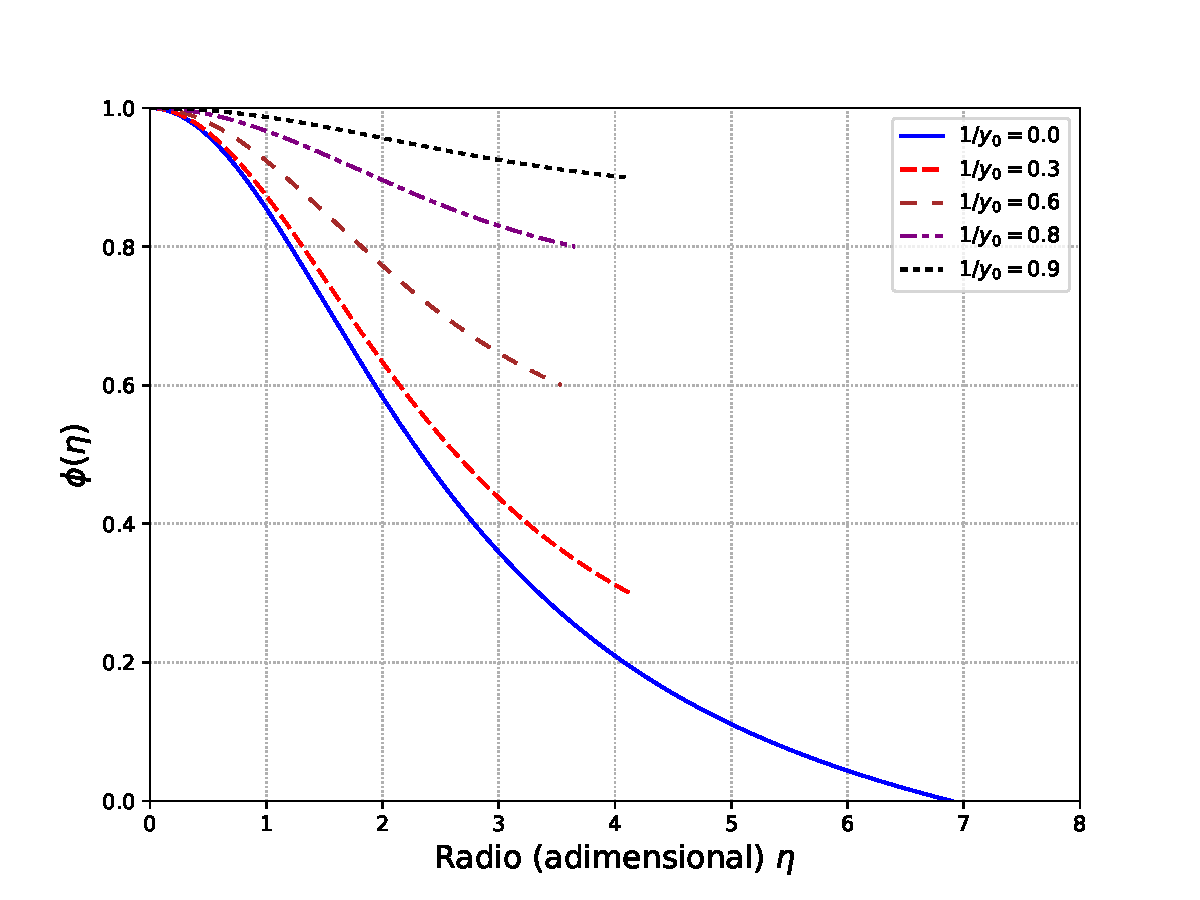
\includegraphics[angle=0,width=0.7\textwidth]{fig/fig-fermi-soluciones.pdf}
\caption{Soluciones $\phi(\eta)$ de la ecuaci'on de estructura de Fermi.}\label{grafico-fermi-soluciones}
\end{figure}



Una importante relaci'on f'isica que se mostrar'a en la siguiente secci'on es la existente entre las masas y radios de las estrellas que obedecen a esta ecuaci'on de estado. Para obtenerla, notamos que la cota superior de las masas est'a dada por la de Chandrasekhar \eqref{ec-fermi-masa-masachandra}, que corresponde a $y_0\to\infty$ 'o $1/y_0=0$. Debido a esto, seleccionamos un conjunto apropiado de valores para este par'ametro, que en nuestro caso son 500 puntos distribuidos uniformemente desde $1/y_0=0$ hasta $1/y_0=0.94$. Esta elecci'on se justifica si recordamos que la condici'on m'inima admisible ser'ia para $1/y_0=1.0$, que corresponder'ia al mismo valor de la condici'on de borde en el origen $\phi(0)=1=1/y_0$, lo que implicar'ia que el radio de la estrella ser'ia nulo: $\eta_1=0$. Luego, los valores de la soluci'on num'erica de la ecuaci'on de estructura por cada uno de estos $y_0$ nos proporcionar'a la cantidad $\eta_1^2\left\Vert\phi'(\eta_1)\right\Vert$, que determina el conjunto de masas estelares admisibles a trav'es de \eqref{ec-fermi-masa-masachandra}: desde un valor m'inimo por conocer, para $y_{\rm 0,min}$, hasta la masa m'axima de Chandrasekhar, para $y_0=\infty$. Por otra parte, del algoritmo de resoluci'on obtendremos tambi'en $\eta_1$ por cada $y_0$, con lo que tendremos los valores del radio de la estrella a trav'es de \eqref{ec-fermi-radio} por cada valor dado de la masa. Por lo tanto, por cada integraci'on num'erica de la ecuaci'on de estructura de Fermi, obtendremos un s'olo punto del diagrama masa-radio, requiri'endose unas 500 en nuestro caso para su determinaci'on con un grado de precisi'on aceptable.

De forma an'aloga tambi'en se determina otra importante relaci'on f'isica que se mostrar'a en la siguiente secci'on: la relaci'on masa-densidad central. En efecto, si mediante el m'etodo anterior obtenemos un conjunto de valores para la masa estelar por cada $y_0$, entonces podemos asociar a cada uno de dichos puntos una densidad central $\rho_{\rm c}$ dada por \eqref{ec-fermi-byrho2}, puesto que depende 'unicamente del par'ametro $y_0$.


\section{Aplicaci'on: Estrellas degeneradas}
En las dos secciones previas se lleg'o a soluciones expl'icitas para la masa y radio de estrellas newtonianas que satisfacen tanto la ecuaci'on de estado de Fermi \eqref{ec-estado-fermi} como las ecuaciones de estado politr'opicas \eqref{estadopolitropica}, que en los casos de $\gamma=5/3$ y $\gamma=4/3$ son aproximaciones de la primera. Ahora bien, hay dos casos simples de estrellas que adoptan naturalmente una ecuaci'on de estado de estos tipos, apropiadas para describir materia degenerada en donde la temperatura no juega un rol relevante (se considera $T=0 K$): las enanas blancas y las estrellas de neutrones. En ellas, la presi'on de materia que contrarresta a la gravitatoria est'a dada por la presi'on de degeneraci'on de sus electrones o neutrones, respectivamente.


\subsection{Enanas blancas}\label{sec:enanasblancas}
Cuando una estrella agota todo el combustible disponible para la fusi'on nuclear, entonces comienza a enfriarse y contraerse, debido a que la presi'on t'ermica no puede contrarrestar la presi'on gravitatoria. La contracci'on tiene como consecuencia que la materia dentro de la estrella se pueda considerar compuesta fundamentalmente de un plasma de n'ucleos at'omicos y electrones degenerados que obedecen a la estad'istica de Fermi-Dirac. Este gas ser'a m'as ideal, es decir, la interacci'on electromagn'etica entre los n'ucleos y los electrones ser'a m'as despreciable (predominando 'unicamente la degeneraci'on de electrones), cuanto m'as alta sea la densidad de la materia considerada. Por lo tanto, cuando la temperatura es suficientemente baja, 'estos 'ultimos pueden ser modelados en primera aproximaci'on como un gas ideal de Fermi completamente degenerado, en donde la principal contribuci'on a la densidad de masa proviene de los n'ucleos at'omicos. En estas circunstancias, es v'alida la ecuaci'on de estado de Fermi exacta y sus aproximaciones politr'opicas  relativista y ultrarelativista (con 'indices politr'opicos $\gamma=5/3$ y $\gamma=4/3$), desarrolladas en el ap'endice \ref{sec:ecsdeestado}.

\subsubsection{Masas y Radios}
Por lo tanto, podemos reemplazar dichas ecuaciones de estado para electrones en las relaciones radio y masa con respecto a la densidad central, y tambi'en en la expresi'on masa-radio de los dos cap'itulos anteriores, adem'as de los resultados num'ericos  de Lane-Emden resumidos en las ra'ices $x_1$ y $x_1^2\left|\Theta(x_1')\right|$ de la tabla \ref{tablalaneemden}, obteniendo las siguientes expresiones que se comparar'an gr'aficamente\footnote{En las relaciones mostradas, se ha usado como normalizaci'on el radio solar $R_{\odot}=6.955\cdot 10^{8}\,[m]$ y la masa solar $M_{\odot}=1.99\cdot10^{30}\,[kg]$.}:

\begin{enumerate}

 \item \emph{Caso no relativista, baja densidad} ($\gamma=5/3$ y $\rho_{\rm c}\ll10^{9}\,[kg/m^3]$).
Aqu'i usamos la constante $K$ para electrones dada en \eqref{fermi_norelativista}
\begin{itemize}
 \item \emph{Radio}:
Reemplazando $K$ en \eqref{radio5/3}, tenemos la siguiente relaci'on radio-densidad central:
\begin{align}
R&=\left(\frac{3^{2/3}\cdot\pi^{1/3}}{8}\frac{\hbar^2}{Gm_e m_u^{5/3}}\right)^{1/2}x_1\,\mu_e^{-5/6}\rho_{\rm c}^{-1/6}\\
% &\approx 3.5470\cdot10^{5}\cdot \left(\frac{\mu_e}{2}\right)^{-5/6}\rho_{\rm c}^{-1/6}\\
% &\approx 0.5010\cdot \left(\frac{\mu_e}{2}\right)^{-5/6}\rho_{\rm c}^{-1/6}\,R_{\odot},\\%0.90871
 &\approx1.1216\cdot10^{4}\left[\frac{\rho_{\rm c}}{10^{9}\,[kg/m^3]}\right]^{-1/6}\left(\frac{\mu_e}{2}\right)^{-5/6}\,[km].
\end{align}
\item \emph{Masa}:
Reemplazando $K$ en \eqref{masa5/3}, tenemos la siguiente relaci'on masa-densidad central:
\begin{align}
M&=4\pi\left(\frac{3^{2/3}\pi^{1/3}}{8}\frac{\hbar^2}{Gm_e m_u^{5/3}}\right)^{3/2}x_1^2\left|\Theta(x_1')\right|\mu_e^{-5/2}\rho_{\rm c}^{1/2}\\
&\approx1.5687\cdot 10^{-5}\,\left(\frac{\mu_e}{2}\right)^{-5/2}\rho_{\rm c}^{1/2}\,M_{\odot}\label{enanablanca5/3-masadensidad}\\
&\approx0.4961\cdot\left[\frac{\rho_{\rm c}}{10^{9}\,[kg/m^3]}\right]^{1/2}\left(\frac{\mu_e}{2}\right)^{-5/2}\,M_{\odot}.
\end{align}
Y reemplazando $K$ en \eqref{masaradio5/3}, obtenemos la siguiente relaci'on masa-radio:
\begin{align}
 M&=\frac{3^2\pi^2}{2^7}\left(\frac{\hbar^2}{Gm_em_u^{5/3}}\right)^3\,x_1^3\,x_1^2\left|\Theta(x_1')\right|\mu_e^{-5} R^{-3}\\
% \frac{M}{M_{\odot}}&=132.384\frac{3^2\pi^2}{2^7}\left(\frac{\hbar^2}{R_{\odot}Gm_em_u^{5/3}}\right)^3 M_{\odot}^{-1}\mu_e^{-5} \left(\frac{100R}{R_{\odot}}\right)^{-3}\\
&\approx7.001\cdot10^{11}\,\left(\frac{\mu_e}{2}\right)^{-5} \left[\frac{R}{1\,[km]}\right]^{-3}M_{\odot} \label{enanablanca5/3-masaradio}\\
% &\approx 2.0809\,\left(\frac{\mu_e}{2}\right)^{-5} \left(\frac{100R}{R_{\odot}}\right)^{-3}M_{\odot}, \label{enanablanca5/3-masaradio}\\
&\approx0.7001\cdot\left[\frac{R}{10^{4}\,[km]}\right]^{-3}\left(\frac{\mu_e}{2}\right)^{-5}\,M_{\odot}.
\end{align}
Recordemos que debido a la discusi'on de la secci'on \eqref{sec:casos-lane-emden}, en este caso tendremos que $MV=cte$, es decir, el volumen de una enana blanca es inversamente proporcional a su masa. Esta afirmaci'on proviene del hecho que la estrella se soporta contra el colapso gravitatorio debido a la presi'on de degeneraci'on de los electrones. 'Estos deben estar m'as cercanamente confinados (menor volumen) para generar una presi'on de degeneraci'on m'as grande (de acuerdo con el principio de exclusi'on de Pauli), necesaria para soportar una estrella m'as masiva.
\end{itemize}

 \item \emph{Caso ultra-relativista, alta densidad} ($\gamma=4/3$ y $\rho_{\rm c}\gg10^{9}\,[kg/m^3]$). Aqu'i usamos la constante $K$ para electrones dada en \eqref{fermi_relativista}.
\begin{itemize}
 \item \emph{Radio}: Reemplazando $K$ en \eqref{radio4/3}, tenemos la siguiente relaci'on radio-densidad central:
\begin{align}
R&=\left(\frac{3^{1/3}}{4\pi^{1/3}}\frac{\hbar c}{Gm_u^{4/3}}\right)^{1/2}x_1\,\mu_e^{-2/3}\,\rho_{\rm c}^{-1/3}\\
% &\approx3.3462\cdot10^{8}\cdot\left(\frac{\mu_e}{2}\right)^{-2/3}\,\rho_{\rm c}^{-1/3}\,[km]\\
% &\approx 48.112\cdot\left(\frac{\mu_e}{2}\right)^{-2/3}\,\rho_{\rm c}^{-1/3}R_{\odot}\\
 &\approx3.3461\cdot10^{4}\left[\frac{\rho_{\rm c}}{10^{9}\,[kg/m^3]}\right]^{-1/3}\left(\frac{\mu_e}{2}\right)^{-2/3}\,[km],
\end{align}
\item \emph{Masa}: Para este valor del 'indice politr'opico, tenemos que la masa, denominada de Chandrasekhar, representa un valor l'imite (ver secci'on \eqref{sec:ec-fermi-masalimite}), es independiente tanto de la densidad central como del radio de la estrella, y su valor se obtendr'a reemplazando $K$ en \eqref{masachandra2} 'o \eqref{masa4/3}:
\begin{align}\label{masachandra}
M_{ch}&=\frac{\sqrt{3\pi}}{2}\left(\frac{\hbar c}{Gm_u^{4/3}}\right)^{3/2}x_1^2\left|\Theta(x_1')\right|\mu_e^{-2}\\
 &\approx1.4562\cdot\left(\frac{\mu_e}{2}\right)^{-2}\,M_{\odot},\label{enanablanca4/3-masa}
\end{align}
de donde vemos que la masa de Chandrasekhar depende 'unicamente de la composici'on de la enana blanca a trav'es del peso molecular medio por electr'on $\mu_e$. Para estrellas compuestas de helio o carbono, donde $\mu_e=2$, su valor es $M_{ch}\approx1.45M_{\odot}$.
\end{itemize}

\item \emph{Ec. de estado de Fermi exacta}. En este caso usamos los resultados obtenidos en la secci'on \eqref{sec:fermi-exacta}.
\begin{itemize}
\item \emph{Radio}: Reemplazando las constantes $A$ \eqref{ec-fermi-A} y $B$ \eqref{ec-fermi-B} para el caso de electrones en la definici'on de $a$ \eqref{ec-fermi-a}, y 'esta en la expresi'on para el radio \eqref{ec-fermi-radio}, tenemos la siguiente relaci'on del radio con el par'ametro $y_0$ y el radio adimensional $\eta_1$:
\begin{align}
R&=\frac{1}{2}\sqrt{\frac{3\pi}{cG}}\frac{\hbar^{3/2}}{ m_e m_u \mu_e}\left(\frac{\eta_1}{y_0}\right)\\
&=3.8849\cdot10^3\left(\frac{\mu_e}{2}\right)^{-1}\left(\frac{\eta_1}{y_0}\right)\;[km].\label{enanablanca-exacta-radio}
% &=0.55858\left(\frac{\mu_e}{2}\right)^{-1}\left(\frac{\eta_1}{y_0}\right)\;\frac{R_{\odot}}{100}.\label{enanablanca-exacta-radio}
\end{align}
\item \emph{Masa}: Podemos expresar la masa de las enanas blancas en t'erminos de la masa l'imite de Chandrasekhar \eqref{enanablanca4/3-masa} mediante la relaci'on \eqref{ec-fermi-masa-masachandra}. Al reemplazar los valores correspondientes de la tabla \ref{tablalaneemden}, obtenemos la siguiente relaci'on de la masa con el valor caracter'istico $\eta_1^2\left\Vert\phi'(\eta_1)\right\Vert$:
\begin{align}
M&=\frac{\eta_1^2\left\Vert\phi'(\eta_1)\right\Vert}{x_1^2\left\Vert\Theta_3'(x_1)\right\Vert}\,M_{ch}\\
&\approx0.72122\left(\frac{\mu_e}{2}\right)^{-2}\eta_1^2\left\Vert\phi'(\eta_1)\right\Vert\, M_{\odot}.\label{enanablanca-exacta-masa}
\end{align}
\item \emph{Densidad central}: Reemplazando el valor de $B$ dado por \eqref{ec-fermi-B} (para electrones) en \eqref{ec-fermi-byrho2}, obtenemos la siguiente relaci'on de la densidad central con el par'ametro $y_0$:
\begin{align}
\rho_{\rm c}&=\frac{m_e^3 c^3}{3\pi^2\hbar^3}m_u\mu_e(y_0^2-1)^{3/2}\\
&\approx1.9478\cdot10^{9}\left(\frac{\mu_e}{2}\right)\,(y_0^2-1)^{3/2}\,[kg/m^3].\label{enanablanca-exacta-densidad}
\end{align}
\end{itemize}


\end{enumerate}

\subsubsection{Gr'aficos y comparaci'on entre modelos exactos y aproximados}
A continuaci'on, puede apreciarse el gr'afico \ref{graficomasa-radio}, donde se muestra la relaci'on masa-radio para enanas blancas (con el valor caracter'istico para el peso molecular medio por electr'on $\mu_e=2$), obtenida directamente por las relaciones provenientes de las ecuaciones de estado aproximadas \eqref{enanablanca5/3-masaradio} y \eqref{enanablanca4/3-masa}, adem'as de la hallada a partir de la soluci'on num'erica de la ecuaci'on de estado de Fermi exacta por medio del m'etodo descrito en la subsecci'on \ref{sec:fermi-numerico}, donde se usan los valores de \eqref{enanablanca-exacta-masa} y \eqref{enanablanca-exacta-radio}.

\begin{figure}[H]
\centering
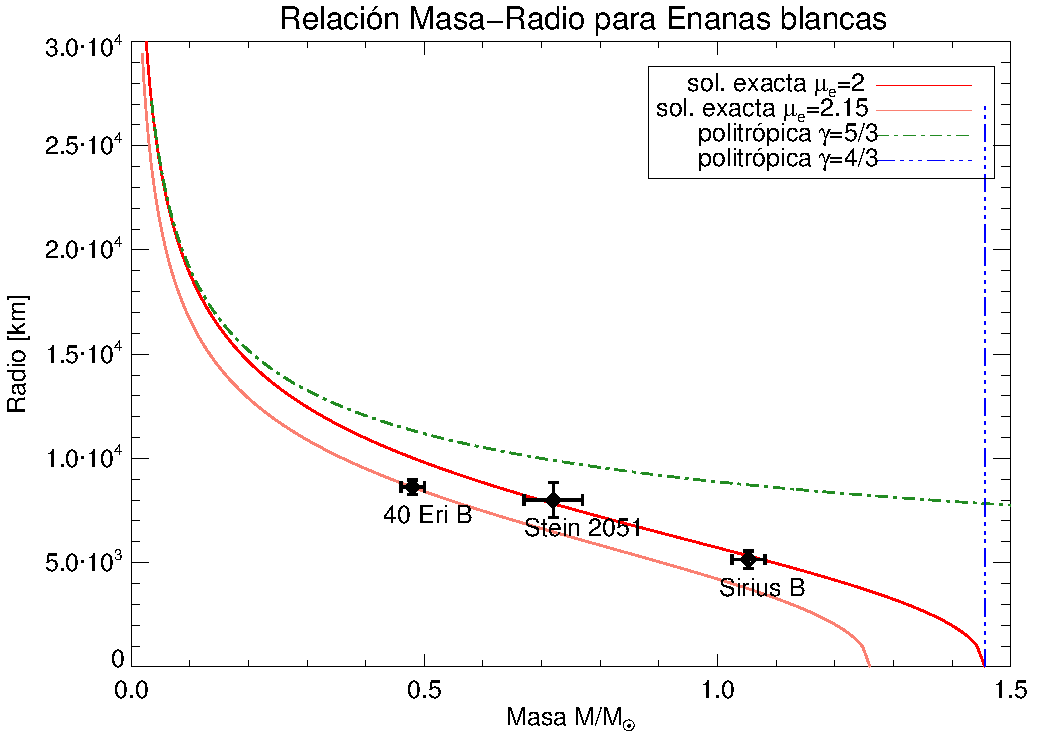
\includegraphics[angle=0,width=0.7\textwidth]{fig/fig-fermielectron-masa-radio.pdf}
\caption{Relaci'on masa-radio para enanas blancas compuestas un gas de electrones completamente degenerado en los casos l'imite no relativista ($\gamma=5/3$) y ultra relativista ($\gamma=4/3$).}\label{graficomasa-radio}
\end{figure}

En primer lugar se debe notar que la masa y el radio obtenidas de la relaci'on exacta para enanas blancas, son inversamente proporcional para todo valor del radio. Adem'as, en la regi'on de radios grandes, la curva exacta se superpone a la correspondiente al caso no relativista, por lo que 'esta es una buena aproximaci'on para radios de enanas blancas mayores a unos 15000 km. (2\% del radio solar), que corresponden a masas del orden de un 20\% de la correspondiente al Sol. Estos cantidades representan entonces los valores t'ipicos para estos par'ametros en este tipo de estrellas.

Por otra parte, cuando el radio de una enana blanca comienza a disminuir por debajo de unos 10000 km (1.5 \% del radio solar), la curva no relativista comienza a diferenciarse notoriamente del resultado exacto, indicando que se est'a entrando en el rango de validez de la aproximaci'on ultra relativista. 'Esta es una buena aproximaci'on para radios menores que unos 5000 km. (similar al radio de la Tierra), pues predice que la masa tiende al valor l'imite de la masa de Chandrasekhar $M_{ch}$ dado en \eqref{enanablanca4/3-masa}. N'otese que, mediante la curva exacta, se observa claramente lo mencionado en la secci'on \ref{sec:ec-fermi-masalimite}: la masa de Chandrasekhar s'olo se alcanza cuando el radio estelar tiende a cero, que es cuando el par'ametro $y_0$ de la ecuaci'on de estructura de Fermi tiende a infinito.

La 'ultima afirmaci'on del p'arrafo anterior implica que la densidad media de la estrella, y por ende la densidad central, (recordar que debido a \eqref{ec-fermi-densidadmediaycentral} ambas cantidades son proporcionales) tender'an a infinito, por lo que es relevante conocer qu'e relaci'on existe entre la masa y densidad central de las enanas blancas. Esto se representa en el gr'afico (\ref{graficomasa-densidad}), donde se muestra dicha relaci'on obtenida directamente por las relaciones provenientes de las ecuaciones de estado aproximadas \eqref{enanablanca5/3-masadensidad} y \eqref{enanablanca4/3-masa}, adem'as de la hallada a partir de la soluci'on num'erica de la ecuaci'on de estado de Fermi exacta  por medio del m'etodo descrito en la subsecci'on \ref{sec:fermi-numerico}, donde se usan los valores \eqref{enanablanca-exacta-masa} y \eqref{enanablanca-exacta-densidad}.

\begin{figure}[H]
\centering
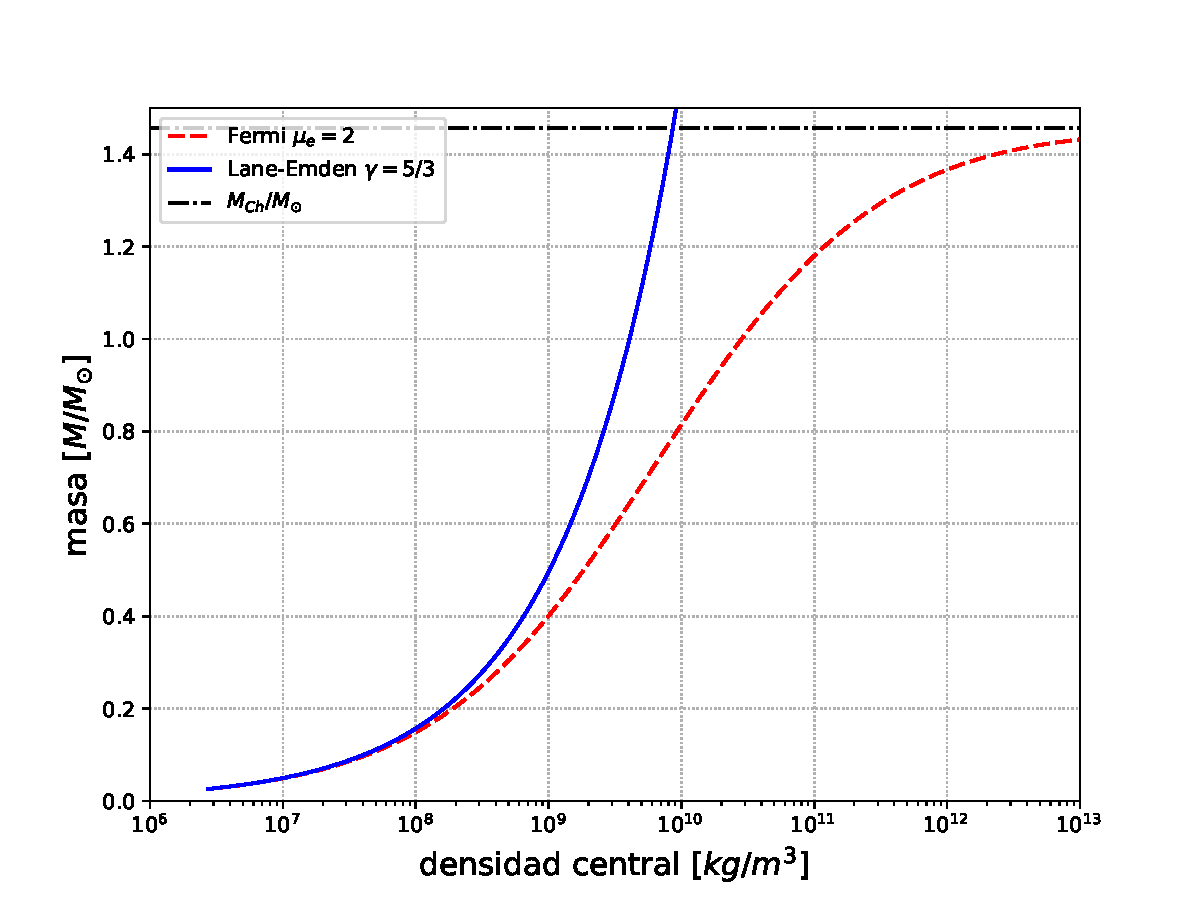
\includegraphics[angle=0,width=0.7\textwidth]{fig/fig-fermielectron-masa-densidad.pdf}
\caption{Relaci'on masa-densidad central para enanas blancas compuestas un gas de electrones completamente degenerado en los casos l'imite no relativista ($\gamma=5/3$) y ultra relativista ($\gamma=4/3$).}\label{graficomasa-densidad}
\end{figure}

La primera caracter'istica relevante que se observa de la curva exacta es que la masa es mon'otonamente creciente con respecto a la densidad central. A'un m'as importante es el hecho que aqu'i se pueden ver claramente los rangos de validez de las aproximaciones efectuadas: el caso no relativista se determin'o haciendo la aproximaci'on $\rho_{\rm c}\ll10^{9}\,[kg/m^3]$, mientras que el ultra relativista se obtuvo para $\rho_{\rm c}\gg10^{9}\,[kg/m^3]$, y consistemente, ambos casos l'imite se superponen a la curva exacta en sus dominios correspondientes. Sin embargo, la curva de la aproximaci'on no relativista es ya muy cercana a la exacta tan s'olo para un orden de magnitud menor de densidades centrales que la densidad cr'itica, mientras que la aproximaci'on ultra relativista posee el mismo margen de exactitud para m'as de tres 'ordenes de magnitud por encima del mismo valor.

La raz'on f'isica del comportamiento anterior se puede entender del siguiente modo: en el rango no relativista, es v'alida la relaci'on masa volumen $MV={\rm cte}$ (\eqref{masavolumen5/3}), por lo que agregando cada vez m'as masa a enanas blancas de baja densidad, dichos astros se encoger'ian proporcionalmente, pero sin l'imite: eventualmente alcanzar'ian $R\to 0$ y $M\to\infty$ (ver gr'afico \ref{graficomasa-radio}), resultando por tanto en una densidad central claramente divergente (ver gr'afico \ref{graficomasa-densidad}). Pero este comportamiento no ocurre debido a que cuando las densidades en el interior de estas estrellas exceden los $10^{9}\,[kg/m^3]$, los electrones se encuentran tan cercanamente confinados que, debido al principio de exclusi'on de Pauli, estos obtendr'ian un momentum tal que dar'ia como resultado velocidades cercanas a las de la luz. Por esta raz'on es que se entra en el rango relativista para densidades mayores que la cr'itica, en donde se observa (ver gr'afico \ref{graficomasa-densidad}) que la masa se aproxima asint'oticamente a la de Chandrasekhar s'olo cuando  $\rho_{\rm c}\to\infty$, que es consistente con el hecho antes mencionado que el radio debe ser nulo para que se logre dicha condici'on.


\subsection{Estrellas de neutrones}

Seg'un el argumento de la secci'on previa, a medida que la densidad de una enana blanca se incrementa en el dominio relativista, se deber'ia obtener la masa l'imite de Chandrasekhar. Pero 'esta nunca se alcanza, pues antes de ello las extremas densidades presentes en el n'ucleo estelar producen un tipo de reacci'on nuclear conocido como decaimiento beta inverso\footnote{Esta reacci'on nuclear es predominante cuando las densidades centrales de las enanas blancas superan los $4\cdot10^{14}\;[kg/m^3]$, mientras que la presi'on de degeneraci'on es dominada por neutrones para densidades mayores a $4\cdot10^{15}\;[kg/m^3]$. Para detalles, ver cap'itulo 3 del texto de Shapiro \cite{Shapiro83}. }:
\begin{equation}
 p+e^{-}\quad\longrightarrow\quad n+\nu_{e},
\end{equation}
lo que cambia la composici'on de la enana blanca antes de su colapso total a una compuesta fundamentalmente por neutrones, donde el nuevo estado de equilibrio se alcanza debido a la presi'on de degeneraci'on de estos fermiones, form'andose as'i las estrellas de neutrones. Por lo tanto, 'estas se pueden modelar en primera aproximaci'on como un gas ideal de neutrones completamente degenerado, donde la masa total se debe 'unicamente s'olo a ellos. En estas circunstancias, es v'alida la misma ecuaci'on de estado de Fermi exacta y sus aproximaciones politr'opicas no relativista ($\gamma=4/3$) y ultra relativista ($\gamma=5/3$), en donde s'olo cambian las constantes referidas a neutrones en vez de a electrones.

\subsubsection{Masas y Radios}
Siguiendo el mismo desarrollo que para enanas blancas, podemos obtener las siguientes relaciones para los radios y masas de estrellas de neutrones, en sus dos aproximaciones caracter'isticas delimitadas por el valor de $x_F$ en \eqref{xrelativo_neutrones}:

\begin{enumerate}

\item \emph{Caso no relativista, baja densidad} ($\gamma=5/3$ y $\rho_{\rm c}\ll6\cdot10^{18}\,[kg/m^3]$).
Aqu'i usamos la constante $K$ para neutrones dada en \eqref{fermi_norelativista2}.
\begin{itemize}
 \item \emph{Radio}:
Reemplazando $K$ en \eqref{radio5/3}, tenemos la siguiente relaci'on radio-densidad central:
\begin{align}
R&=\left(\frac{3^{2/3}\cdot\pi^{1/3}}{8}\frac{\hbar^2}{G m_n^{5/3}}\right)^{1/2}x_1\,\rho_{\rm c}^{-1/6}\\
% &\approx 0.02104\cdot \rho_{\rm c}^{-1/6}\,R_{\odot},\\%0.90871
 &\approx14.633\left[\frac{\rho_{\rm c}}{10^{18}\,[kg/m^3]}\right]^{-1/6}\,[km].
\end{align}
\item \emph{Masa}:
Reemplazando $K$ en \eqref{masa5/3}, tenemos la siguiente relaci'on masa-densidad central:
\begin{align}
M&=4\pi\left(\frac{3^{2/3}\pi^{1/3}}{8}\frac{\hbar^2}{G m_n^{8/3}}\right)^{3/2}x_1^2\left|\Theta(x_1')\right|\rho_{\rm c}^{1/2}\\
&\approx1.1015\cdot 10^{-9}\,\rho_{\rm c}^{1/2}\,M_{\odot}\label{neutrones5/3-masadensidad}\\
&\approx1.1015\cdot\left[\frac{\rho_{\rm c}}{10^{18}\,[kg/m^3]}\right]^{1/2}\,M_{\odot}.
\end{align}
Y reemplazando $K$ en \eqref{masaradio5/3}, obtenemos la siguiente relaci'on masa-radio:
\begin{align}
 M&=\frac{3^2\pi^2}{2^7}\left(\frac{\hbar^2}{Gm_n^{8/3}}\right)^3\,x_1^3\,x_1^2\left|\Theta(x_1')\right| R^{-3}\\
% \frac{M}{M_{\odot}}&=132.384\frac{3^2\pi^2}{2^7}\left(\frac{\hbar^2}{R_{\odot}Gm_em_u^{5/3}}\right)^3 M_{\odot}^{-1}\mu_e^{-5} \left(\frac{100R}{R_{\odot}}\right)^{-3}\\
% &\approx 10.2601\, \left(\frac{10^5 R}{R_{\odot}}\right)^{-3}M_{\odot}, \\
&\approx3.4518\cdot\left[\frac{R}{10\,[km]}\right]^{-3}\,M_{\odot}.\label{neutrones5/3-masaradio}
\end{align}

\end{itemize}

 \item \emph{Caso ultra-relativista, alta densidad} ($\gamma=4/3$ y $\rho_{\rm c}\gg6\cdot10^{18}\,[kg/m^3]$). Aqu'i usamos la constante $K$ para neutrones dada en \eqref{fermi_relativista2}
\begin{itemize}
 \item \emph{Radio}: Reemplazando $K$ en \eqref{radio4/3}, tenemos la siguiente relaci'on radio-densidad central:
\begin{align}
R&=\left(\frac{3^{1/3}}{4\pi^{1/3}}\frac{\hbar c}{Gm_n^{4/3}}\right)^{1/2}x_1\,\rho_{\rm c}^{-1/3}\\
% &\approx 75.935\,\rho_{\rm c}^{-1/3}R_{\odot}\\
 &\approx52.813\left[\frac{\rho_{\rm c}}{10^{18}\,[kg/m^3]}\right]^{-1/3}\,[km].
\end{align}
\item \emph{Masa}: La masa de este caso l'imite, denominada de Chandrasekhar, se obtendr'a reemplazando $K$ en \eqref{masachandra2} 'o \eqref{masa4/3}:
\begin{align}\label{masachandra-neutrones}
M_{ch}&=\frac{\sqrt{3\pi}}{2}\left(\frac{\hbar c}{Gm_n^{4/3}}\right)^{3/2}x_1^2\left|\Theta(x_1')\right|\mu_e^{-2}\\
 &\approx5.7252\,M_{\odot},\label{neutrones4/3-masa}
\end{align}
de donde vemos que es aproximadamente 4 veces mayor que la correspondiente masa de Chandrasekhar para enanas blancas \eqref{enanablanca4/3-masa}, considerando $\mu_e=2$.
\end{itemize}

\item \emph{Ec. de estado de Fermi exacta}. Aqu'i usamos los resultados obtenidos en la secci'on \eqref{sec:fermi-exacta}.
\begin{itemize}
\item \emph{Radio}: Reemplazando las constantes $A$ \eqref{ec-fermi-A} y $B$ \eqref{ec-fermi-B} para el caso de neutrones en la definici'on de $a$ \eqref{ec-fermi-a}, y 'esta en la expresi'on para el radio \eqref{ec-fermi-radio}, tenemos la siguiente relaci'on del radio con el par'ametro $y_0$ y el radio adimensional $\eta_1$:
\begin{align}
R&=\frac{1}{2}\sqrt{\frac{3\pi}{cG}}\frac{\hbar^{3/2}}{m_n^2}\left(\frac{\eta_1}{y_0}\right)\\
% &=0.60236\left(\frac{\eta_1}{y_0}\right)\;\frac{R_{\odot}}{10^{5}}.\label{neutrones-exacta-radio}
&=4.18945\left(\frac{\eta_1}{y_0}\right)\,[km].\label{neutrones-exacta-radio}
\end{align}
\item \emph{Masa}: Notando que aqu'i tambi'en es v'alido \eqref{enanablanca-exacta-masa}, pero usando el l'imite de Chandrasekhar para neutrones \eqref{neutrones4/3-masa}, podemos encontrar que:
\begin{align}
M&=\frac{\eta_1^2\left\Vert\phi'(\eta_1)\right\Vert}{x_1^2\left\Vert\Theta_3'(x_1)\right\Vert}\,M_{ch}.\\
&=2.83673\,\eta_1^2\left\Vert\phi'(\eta_1)\right\Vert\, M_{\odot}.\label{neutrones-exacta-masa}
\end{align}
\item \emph{Densidad central}: Reemplazando el valor de $B$ dado en \eqref{ec-fermi-B} para neutrones, en \eqref{ec-fermi-byrho2}, obtenemos la siguiente relaci'on de la densidad central con el par'ametro $y_0$:
\begin{align}
\rho_{\rm c}&=\frac{m_n^4 c^3}{3\pi^2\hbar^3}(y_0^2-1)^{3/2}\\
&=6.10656\cdot10^{18}\,(y_0^2-1)^{3/2}\,[kg/m^3].\label{neutrones-exacta-densidad}
\end{align}
\end{itemize}


\end{enumerate}

\subsubsection{Gr'aficos}
En el gr'afico siguiente se muestra la relaci'on masa-radio para estrellas de neutrones, obtenida directamente por las relaciones provenientes de las ecuaciones de estado aproximadas \eqref{neutrones5/3-masaradio} y \eqref{neutrones4/3-masa}, adem'as de la hallada a partir de la soluci'on num'erica de la ecuaci'on de estado de Fermi exacta por medio del m'etodo descrito en la subsecci'on \ref{sec:fermi-numerico}, donde se usan los valores \eqref{neutrones-exacta-masa} y \eqref{neutrones-exacta-radio}.


\begin{figure}[H]
\centering
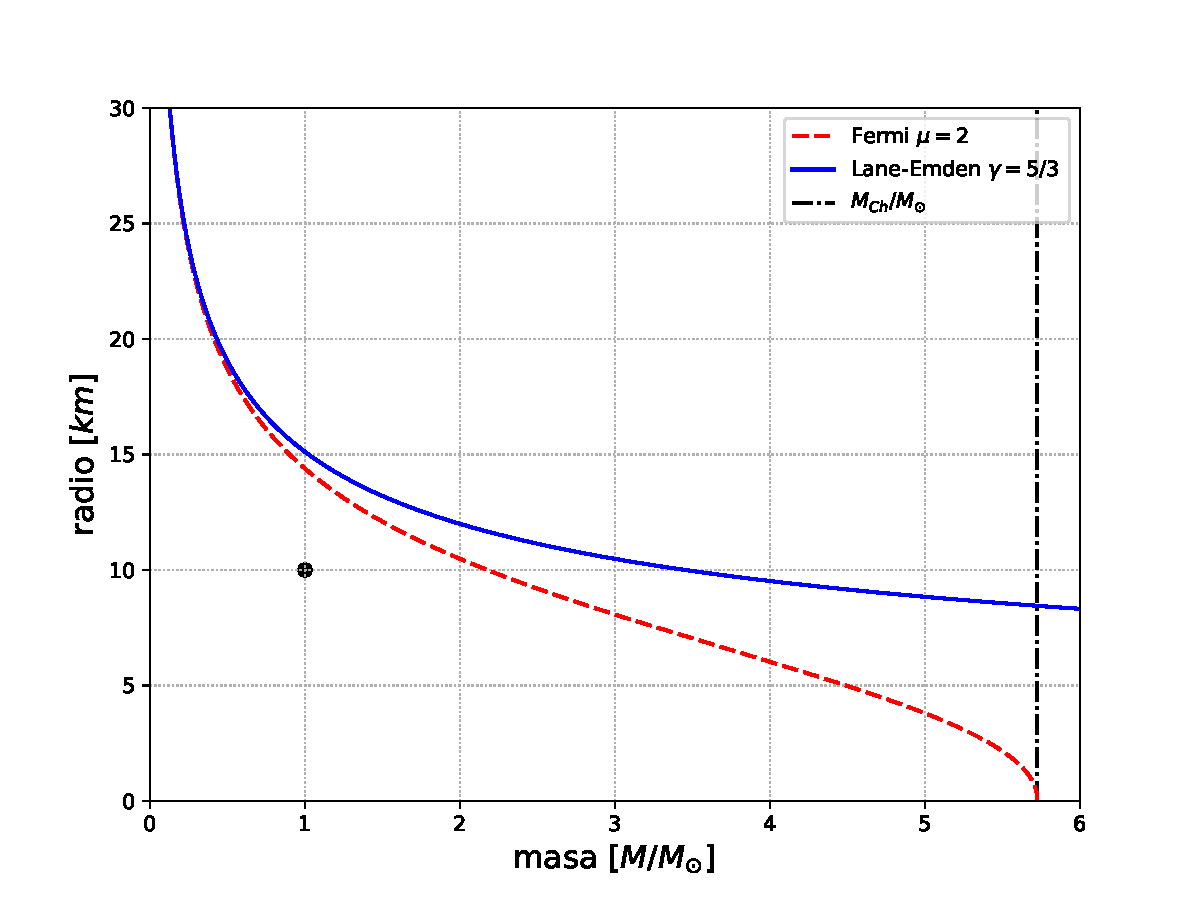
\includegraphics[angle=0,width=0.7\textwidth]{fig/fig-fermineutron-masa-radio.pdf}
\caption{Relaci'on masa-radio para estrellas de neutrones compuestas un gas de neutrones completamente degenerado en los casos l'imite no relativista ($\gamma=5/3$) y ultra relativista ($\gamma=4/3$). Se destaca, adem'as, el valor m'as nombrado en la literatura para la masa y el radio de estas estrellas (1 $M_\odot$, $10[km]$).}\label{graficomasa-radio-neutrones}
\end{figure}

Evidentemente, este gr'afico corresponde s'olo a un reescalamiento del correspondiente a enanas blancas \ref{graficomasa-radio}, siendo v'alidos los mismos comentarios hechos all'i. Por tanto, lo 'unico digno de mencionar es que, si bien las masas t'ipicas de las estrellas de neutrones est'an en torno a una masa solar, sus radios t'ipicos son unas 1000 veces menores que los correspondientes a las enanas blancas, siendo tan s'olo de algunas decenas de kil'ometros.

Por otra parte, en el siguiente gr'afico, se muestra la relaci'on masa-densidad obtenida directamente por las relaciones provenientes de las ecuaciones de estado aproximadas \eqref{neutrones5/3-masadensidad} y \eqref{neutrones4/3-masa}, adem'as de la hallada a partir de la soluci'on num'erica de la ecuaci'on de estado de Fermi exacta por medio del m'etodo descrito en la subsecci'on \ref{sec:fermi-numerico}, donde se usan los valores de \eqref{neutrones-exacta-masa} y \eqref{neutrones-exacta-densidad}.

\begin{figure}[H]
\centering
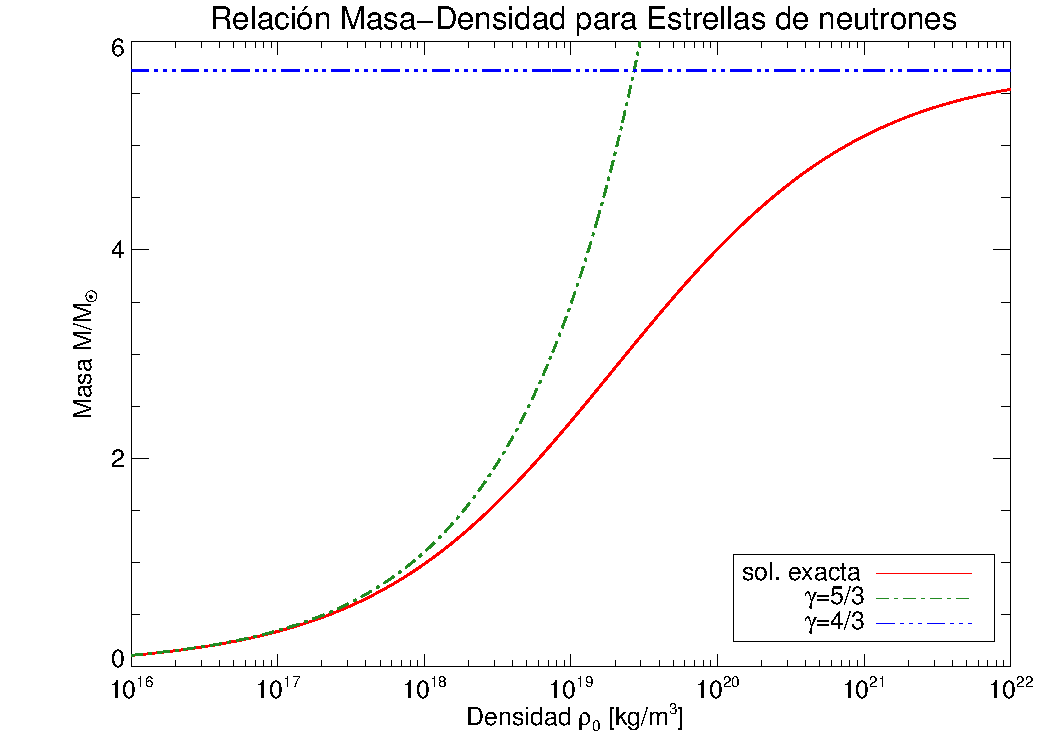
\includegraphics[angle=0,width=0.7\textwidth]{fig/fig-fermineutron-masa-densidad.pdf}
\caption{Relaci'on masa-densidad central estrellas de neutrones compuestas un gas de neutrones completamente degenerado en los casos l'imite no relativista ($\gamma=5/3$) y ultra relativista ($\gamma=4/3$)}\label{graficomasa-densidad-neutrones}
\end{figure}

Obviamente, este gr'afico tambi'en corresponde a un reescalamiento del correspondiente al de las enanas blancas (ver figura \ref{graficomasa-densidad}). Los radios extremadamente peque\~nos que exhiben las estrellas de neutrones mostrados en la figura \ref{graficomasa-radio-neutrones}, implican necesariamente que su densidad debe ser gigantesca: aqu'i se puede ver claramente que sus densidades centrales t'ipicas son del orden de $\rho_{\rm c}\approx10^{18}\,[kg/m^3]$, que corresponden al orden de magnitud de las densidades de los n'ucleos at'omicos. Esto se puede entender al pensar que estos astros est'an compuestos pr'acticamente s'olo de neutrones, tan cercanamente confinados que pr'acticamente no hay espacio entre ellos: es en este sentido que las estrellas de neutrones son como un n'ucleo at'omico gigante.


%\section[Principio variacional]{Energ'ia de una estrella y Principio variacional *}\label{sec:ppio_variacional_newton}
%
%\subsection{Energ'ia de una estrella politr'opica}\label{sec:energia_newton}
%
%En esta subsecci'on se calcular'a expl'icitamente la energ'ia interna $U$ y potencial gravitacional $V$, para una estrella politr'opica que satisface \eqref{estadopolitropica}. La energ'ia total de este sistema ser'a simplemente la suma de ambas.
%
%\subsubsection{Energ'ia potencial gravitacional}
%El c'alculo se har'a de dos formas distintas, las cuales se comparar'an posteriormente para determinar una integral que se utilizar'a para la energ'ia interna:
%\begin{enumerate}
% \item \emph{M'etodo 1: Usando la ecuaci'on de equilibrio hidrost'atico \eqref{eqnewton}.}
%
%La energ'ia potencial gravitatoria total de una estrella se definir'a por:
%\begin{align}\label{energia_potencial_newton}
%V=-\int_0^R\frac{G\mathcal{M}(r)}{r}d\mathcal{M}.
%\end{align}
%Usando \eqref{masa1} para determinar $d\mathcal{M}(r)$ y la ecuaci'on de equilibrio hidrost'atico \eqref{eqnewton} para introducir la presi'on $P$, tenemos que:
%\begin{align}
% V&=-\int\limits_0^R\frac{G\mathcal{M}(r)}{r}\left[4\pi r^2\rho(r)\,dr\right]=-4\pi\int\limits_0^R  r\left[G\mathcal{M}(r)\rho(r)\right]\,dr \label{energia_potencial_newton1}\\
%&=4\pi\int\limits_0^R r\left[-r^2\frac{dP}{dr}\right]\,dr=4\pi\int\limits_0^R r^3\,dP.
%\end{align}
%Integrando por partes, podemos escribir:
%\begin{align}
% V&=4\pi\int\limits_0^R r^3\,dP=4\pi\left[\int\limits_0^R d(Pr^3)-\int\limits_0^R P\,d(r^3)\right]\\
%&=4\pi\left[\cancelto{0}{P(R)}R^3-\lim_{r\to 0}(P(r)\cancelto{0}{r^3})-3\int\limits_0^R P\,r^2\,dr\right]\\
%&=-3\int\limits_0^R P\,4\pi r^2\,dr.\label{energia_potencial1}
%\end{align}
%Si ahora multiplicamos y dividimos por la densidad $\rho$, podemos usar la expresi'on para la masa $\mathcal{M}$ \eqref{masa2}, e integrar nuevamente por partes:
%\begin{align}
% V&=-3\int\limits_0^R \frac{P}{\rho}\,\left[4\pi \rho r^2 \,dr\right]=-3\int\limits_0^R\frac{P}{\rho}d\mathcal{M}\\
%&=-3\int\limits_0^R\left[d\left(\frac{P}{\rho}\mathcal{M}\right)-\mathcal{M}d\left(\frac{P}{\rho}\right)\right]\\
%&=-3\left[\cancelto{0}{\left(\lim_{r\to R}\frac{P}{\rho}\right)}\mathcal{M}-\left(\lim_{r\to 0}\frac{P}{\rho}\cancelto{0}{\mathcal{M}}\right)\right]+3\int\limits_0^R\mathcal{M}\,d\left(\frac{P}{\rho}\right).\label{energia_potencial_2}
%\end{align}
%El primer l'imite se anula debido a que, por la ecuaci'on de estado politr'opica, tendremos la relaci'on siguiente
%\begin{align}
% \frac{P}{\rho}=K\rho^{\gamma-1}\quad\Rightarrow\quad \lim_{r\to R}\left(\frac{P}{\rho}\right)=K[\cancelto{0}{\rho(R)}]^{\gamma-1}=0,
%\end{align}
%para todos los valores f'isicamente aceptables del 'indice politr'opico ($\gamma>6/5$). Con el objetivo de seguir simplificando $V$, primero notamos que
%\begin{align}
% P=K\rho^{\gamma}\qquad\Rightarrow\qquad \rho=\left(\frac{P}{K\rho}\right)^{1/(\gamma-1)}.
%\end{align}
%Con esta relaci'on, es posible expresar el diferencial $d\left(P/\rho\right)$ en t'erminos del diferencial $dP$, pues:
%\begin{align}
% dP&=d(K\rho^{\gamma})=K\gamma\rho^{\gamma-1}d\rho,\\
% &=K\gamma\rho^{\gamma-1}d\left(\frac{P}{K\rho}\right)^{1/(\gamma-1)}\\
%&=\frac{\gamma}{\gamma-1}\rho^{\gamma-1}\left(\frac{P}{K\rho}\right)^{1/(\gamma-1)-1}\,d\left(\frac{P}{\rho}\right)\\
%&=\frac{\gamma}{\gamma-1}\rho^{\gamma-1}\left(\rho^{\gamma-1} \right)^{(2-\gamma)/(\gamma-1)} \,d\left(\frac{P}{\rho}\right)\\
%&=\frac{\gamma}{\gamma-1}\;\rho\;d\left(\frac{P}{\rho}\right).
%\end{align}
%As'i, reemplazando la relaci'on anterior en \eqref{energia_potencial_2} y usando nuevamente la ecuaci'on de equilibrio \eqref{eqnewton}, tenemos:
%\begin{align}
% V&=3\int\limits_0^R\mathcal{M}\,\frac{\gamma-1}{\gamma}\frac{dP}{\rho}=3\frac{\gamma-1}{\gamma}\int\limits_0^R\mathcal{M}\,\left[\frac{1}{\rho}\frac{dP}{dr}\right]\,dr\\
%&=3\frac{\gamma-1}{\gamma}\int\limits_0^R\mathcal{M}\,\left[-\frac{G\mathcal{M}}{r^2}\right]\,dr\\
%&=3G\frac{\gamma-1}{\gamma}\int\limits_0^R\mathcal{M}^2\,d\left(\frac{1}{r}\right).\label{relacion_dp}
%\end{align}
%Integrando por partes, podemos escribir:
%\begin{align}
% V&=3G\frac{\gamma-1}{\gamma}\int\limits_0^R\left[d\left(\frac{\mathcal{M}^2}{r}\right)-d\left(\mathcal{M}^2\right)\frac{1}{r}\right]\\
%&=3G\frac{\gamma-1}{\gamma}\left[\frac{[\mathcal{M}(R)]^2}{R}-\lim_{r\to 0}\cancelto{0}{\left(\frac{\mathcal{M}^2}{r}\right)}-2\int\limits_0^R\,\frac{\mathcal{M}}{r}d\mathcal{M}\right],\\
%&=3\frac{\gamma-1}{\gamma}\left[\frac{GM^2}{R}-2\int\limits_0^R\,\frac{G\mathcal{M}}{r}d\mathcal{M}\right].
%\end{align}
%Vemos que la 'ultima integral la podemos identificar con la expresi'on original para $V$, es decir,
%\begin{align}
% V&=3\frac{\gamma-1}{\gamma}\left[\frac{GM^2}{R}+2V\right],
%\end{align}
%y despejando dicha variable, encontramos una expresi'on expl'icita para la energ'ia potencial gravitatoria en t'erminos de la masa $M$, radio $R$ e 'indice politr'opico $\gamma$ de la estrella:
%\begin{equation}\label{energia_potencial_newton:r1}
% \boxed{V=-3\left(\frac{\gamma-1}{5\gamma-6}\right)\frac{GM^2}{R}.}
%\end{equation}
%Para aplicaciones posteriores es 'util reexpresar la relaci'on anterior eliminando $R$ e introduciendo la densidad central $\rho_{\rm c}$, adem'as de la funci'on adimensional de Lane-Emden $\Theta$ que depende de $\gamma$. Con este objetivo se debe usar la relaci'on \eqref{densidad0politropica}, despejando $1/R$:
%\begin{equation}
% \frac{1}{R}=\left(\frac{4\pi \rho_{\rm c}}{M}\frac{x_1^2\left\Vert\Theta'(x_1)\right\Vert}{x_1^3}\right)^{1/3},
%\end{equation}
%la cual se puede reemplazar en \eqref{energia_potencial_newton:r1}, obteniendo:
%\begin{equation}\label{energia_potencial_newton:r2}
% \boxed{V=-3\left(\frac{\gamma-1}{5\gamma-6}\right)\frac{\left(4\pi x_1^2\left\Vert\Theta'(x_1)\right\Vert\right)^{1/3}}{x_1}GM^{5/3}\rho_{\rm c}^{1/3}.}
%\end{equation}
%\item\emph{Forma 2: Sin asumir la ecuaci'on de equilibrio hidrost'atico newtoniana \eqref{eqnewton}, 'o en t'erminos de variables adimensionales de Lane-Emden.}\\
%Partimos nuevamente de la definici'on de energ'ia potencial gravitatoria como la integral \eqref{energia_potencial_newton1} (en donde s'olo se ha usado la ecuaci'on de masa), pero ahora escribi'endola en t'erminos de las variables adimensionales de Lane-Emden $x$ y $\Theta$ dadas en \eqref{x} y \eqref{theta}. Adem'as, $\mathcal{M}$ se puede reescribir usando \eqref{masapoli-en-r} como:
%\begin{equation}
% \mathcal{M}=\frac{x^2\left\Vert\Theta'(x)\right\Vert}{x_1^2\left\Vert\Theta'(x_1)\right\Vert}M.
%\end{equation}
%Luego, tendremos que:
%\begin{align}
%V&=-4\pi G\int_0^R \mathcal{M}\,\rho\,r\,dr\\
%&=-4\pi G\int_0^{x_1}\left[\frac{x^2\left\Vert\Theta'(x)\right\Vert}{x_1^2\left\Vert\Theta'(x_1)\right\Vert}M\right]\,\left[\rho_{\rm c}\,\Theta^{1/(\gamma-1)}\right](ax)\,d(ax)\\
%&=\frac{4\pi G M\rho_{\rm c}}{x_1^2\left\Vert\Theta'(x_1)\right\Vert}\,a^2\int\limits_0^{x_1}x^3\Theta'(x)\Theta(x)^{1/(\gamma-1)}\,dx.
%\end{align}
%Pero podemos usar \eqref{masaparcial-laneemden} (evaluada en $x=x_1$) para encontrar una expresi'on para la escala de longitud $a$ en t'erminos de las variables antes se\~naladas:
%\begin{equation}
% a=\left(\frac{M}{4\pi\rho_{\rm c} x_1^2\left|\Theta'(x_1)\right|}\right)^{1/3}.
%\end{equation}
%De este modo, encontramos que,
%\begin{align}
% V=\left(4\pi\rho_{\rm c}\right)^{1/3}\frac{GM^{5/3}}{\left(x_1^2\left\Vert\Theta'(x_1)\right\Vert\right)^{5/3}}\int\limits_0^{x_1}x^3\Theta'\Theta^{1/(\gamma-1)}\,dx.
%\end{align}
%Integrando por partes la integral anterior es posible expresarla de una forma m'as compacta:
%\begin{align}
% \int\limits_0^{x_1}x^3\Theta'\Theta^{1/(\gamma-1)}\,dx&=\int\limits_0^{x_1}\frac{x^3}{1/(\gamma-1)+1}\frac{d}{dx}\left(\Theta^{1/(\gamma-1)+1}\right)\,dx\\
%&=\frac{\gamma-1}{\gamma}\left[\int\limits_0^{x_1}d\left(\Theta^{\gamma/(\gamma-1)}x^3\right)-\int\limits_0^{x_1}\Theta^{\gamma/(\gamma-1)}d(x^3)\right]\\
%&=\frac{\gamma-1}{\gamma}\left[[\cancelto{0}{\Theta(x_1)}x_1^3]^{\gamma/(\gamma-1)}-\lim_{x\to 0}\left(\Theta^{\gamma/(\gamma-1)}\cancelto{0}{x}^3\right)-3\int\limits_0^{x_1}x^2\Theta^{\gamma/(\gamma-1)}\,dx\right].
%\end{align}
%Por lo tanto, encontramos que el potencial gravitatorio se puede escribir tambi'en en la forma:
%\begin{align}\label{energia_potencial_politropicac}
% \boxed{V=-\left(4\pi\rho_{\rm c}\right)^{1/3}\frac{GM^{5/3}}{\left(x_1^2\left\Vert\Theta'(x_1)\right\Vert\right)^{5/3}}\,3\frac{\gamma-1}{\gamma}\int\limits_0^{x_1}x^2\Theta^{\gamma/(\gamma-1)}\,dx.}
%\end{align}
%Tambi'en podemos expresar lo anterior en una forma que ser'a 'util en el siguiente cap'itulo, separando la parte dependiente de $\gamma$ de los dem'as par'ametros:
%\begin{equation}\label{energia_potencial_newton-c}
%\boxed{V=-C_2\,M^{5/3}\,\rho_{\rm c}^{1/3}=-G\mathcal{C}_2(\gamma)\,M^{5/3}\,\rho_{\rm c}^{1/3}}
%\end{equation}
%en donde $C_2:=G\mathcal{C}_2$ y
%\begin{equation}\label{energia_coef_c2}
% \mathcal{C}_2(\gamma):=3\frac{\left(4\pi\right)^{1/3}}{x_1^2\left\Vert\Theta'(x_1)\right\Vert}\,\frac{\gamma-1}{\gamma}\int\limits_0^{x_1}x^2\Theta^{\gamma/(\gamma-1)}\,dx.
%\end{equation}
%
%
%Ser'a 'util tambi'en determinar el valor de la integral que aparece en la 'ultima ecuaci'on en t'erminos de funciones de Lane-Emden simples. Para ello, simplemente se igualan las relaciones para $V$ antes halladas en \eqref{energia_potencial_newton:r2} y \eqref{energia_potencial_politropicac}, obteniendo:
%\begin{align}
%%  V&=-\left(4\pi\rho_{\rm c}\right)^{1/3}\frac{GM^{5/3}}{x_1^2\left\Vert\Theta'(x_1)\right\Vert}\,3\frac{\gamma-1}{\gamma}\int\limits_0^{x_1}x^2\Theta^{\gamma/(\gamma-1)}\,dx=-3\left(\frac{\gamma-1}{5\gamma-6}\right)\frac{\left(4\pi x_1^2\left\Vert\Theta'(x_1)\right\Vert\right)^{1/3}}{x_1}GM^{5/3}\rho_{\rm c}^{1/3}\\
%\int\limits_0^{x_1}x^2\Theta^{\gamma/(\gamma-1)}\,dx=\frac{\gamma}{5\gamma-6}\frac{\left(x_1^2\left\Vert\Theta'(x_1)\right\Vert\right)^2}{x_1}.\label{integral_laneemden}
%\end{align}
%
%
%
%\end{enumerate}
%
%\subsubsection{Energ'ia interna}
%Si definimos la energ'ia interna por unidad de volumen ('o densidad de energ'ia interna) como $u(r)=dU(r)/dV$, tendremos que la energ'ia interna total de la estrella ser'a:
%\begin{align}\label{energia_interna_newton}
% U&=\int\limits_0^R \,u(r)\,dV=\int\limits_0^R 4\pi r^2\,u(r)\,dr.
%\end{align}
%Reemplazando la ecuaci'on de estado politr'opica \eqref{estadopolitropica_alterna}, que relaciona $u$  con $P$,  en la relaci'on anterior, tenemos
%\begin{align}\label{energia_interna1}
%U&=\frac{1}{\gamma-1}\int\limits_0^R P\, 4\pi r^2 \,dr.
%\end{align}
%
%\begin{enumerate}
% \item \emph{Forma 1: Usando la definici'on de energ'ia potencial gravitacional}\\
%En \eqref{energia_interna1}, podemos identificar la expresi'on para la energ'ia potencial gravitacional dada en \eqref{energia_potencial1}, de donde obtenemos la relaci'on entre ambos tipos de energ'ias:
%\begin{align}
%U&=-\frac{V}{3(\gamma-1)},\label{energia_int_pot}
%\end{align}
%con la cual, de la expresi'on expl'icita para $V$ dada en \eqref{energia_potencial_newton:r1}, encontramos finalmente para la energ'ia interna de una estrella politr'opica:
%\begin{equation}\label{energia_interna_newton:r1}
% \boxed{U=\frac{1}{5\gamma-6}\frac{GM^2}{R}.}
%\end{equation}
%
%\item \emph{Forma 2: Sin asumir la ecuaci'on de equilibrio hidrost'atico, 'o en t'erminos de variables adimensionales.}\\
%Podemos expresar \eqref{energia_interna1} en funci'on de $x$ y $\Theta$ mediante sus definiciones \eqref{x}, \eqref{theta} y la ecuaci'on de estado politr'opica:
%\begin{align}
% U&=\frac{1}{\gamma-1}\int\limits_0^R K\rho^{\gamma}\, 4\pi (ax)^2 \,d(ax)=\frac{4\pi a^3 K}{\gamma-1}\int\limits_0^{x_1}\left(\rho_{\rm c}\Theta^{1/(\gamma-1)}\right)^{\gamma}\,x^2\,dx\\
%&=\frac{\left(4\pi\rho_{\rm c}\, a^3\right)}{\gamma-1}K\rho_{\rm c}^{\gamma-1}\int\limits_0^{x_1}x^2\,\Theta^{\gamma/(\gamma-1)}\,dx.
%\end{align}
%Usando \eqref{masaparcial-laneemden} evaluada en $x=x_1$, es posible reescribir la cantidad entre par'entesis anterior en t'erminos de $M$, y la integral se puede calcular en funci'on de \eqref{integral_laneemden}, de modo que:
%\begin{align}
% U=\frac{M}{x_1^2\left|\Theta'(x_1)\right|}\frac{K\rho_{\rm c}^{\gamma-1}}{\gamma-1}\left[\frac{\gamma}{5\gamma-6}\frac{(x_1^2\left|x_1^2\Theta'(x_1)\right|)^2}{x_1}\right].
%\end{align}
%Entonces, tenemos que la energ'ia interna total ser'a:
%\begin{align}\label{energia_interna_newton:r2}
% \boxed{U=\frac{\gamma/(\gamma-1)}{5\gamma-6}\,\frac{x_1^2\left|\Theta'(x_1)\right|}{x_1}\, KM\,\rho_{\rm c}^{\gamma-1}.}
%\end{align}
%
%De la misma forma que en el caso anterior, podemos separar esta expresi'on en una parte dependiente de $\gamma$ y otra de los par'ametros:
%\begin{equation}\label{energia_interna_newton-c}
% \boxed{U=C_1\,M\,\rho_{\rm c}^{\gamma-1}=K\,\mathcal{C}_1(\gamma)\,M\,\rho_{\rm c}^{\gamma-1}.}
%\end{equation}
%en donde $C_1:=K\mathcal{C}_1(\gamma)$ y
%\begin{equation}\label{energia_coef_c1}
% \mathcal{C}_1(\gamma):=\frac{\gamma/(\gamma-1)}{5\gamma-6}\,\frac{x_1^2\left|\Theta'(x_1)\right|}{x_1}.
%\end{equation}
%
%\end{enumerate}
%
%
%\subsubsection{Energ'ia total}
%De las relaciones anteriores \eqref{energia_interna_newton:r1} y \eqref{energia_potencial_newton:r1} podremos determinar una expresi'on para una estrella newtoniana que obedece la ecuaci'on de estado \eqref{estadopolitropica} con 'indice politr'opico $\gamma$:
%\begin{align}\label{energia_total_newtoniana}
% \boxed{E=U+V=(4-3\gamma)U=-\frac{3\gamma-4}{5\gamma-6}\frac{GM^2}{R}.}
%\end{align}
%De aqu'i es posible deducir que la energ'ia de la estrella ser'a negativa si $\gamma>4/3$, mientras que $E>0$ si $6/5<\gamma<4/3$\footnote{Recordar que el caso $\gamma<6/5$ no es f'isicamente relevante, pues la estrella tendr'ia radio infinito.}.
%
%La energ'ia total tambi'en se puede obtener sumando las expresiones alternas para las energ'ias interna y potencial gravitatoria \eqref{energia_interna_newton-c} y \eqref{energia_potencial_newton-c}:
%\begin{equation}\label{energia_newton}
%\boxed{ E=U+V=C_1\, M\rho_{\rm c}^{\gamma-1}-C_2\,M^{5/3}\rho_{\rm c}^{1/3}.}
%\end{equation}
%
%\subsection{Ecuaci'on de equilibrio hidrost'atico de un principio variacional}
%
%
%
%En esta secci'on, se probar'a que el hecho que la energ'ia $E$ de una estrella compuesta de un fluido ideal (con composici'on qu'imica y entrop'ia por bari'on constante) sea extremal ('o un punto cr'itico, 'o estacionario), es equivalente a la condici'on de equilibrio hidrost'atico dada por la ecuaci'on \eqref{eqnewton}. Este resultado se aplicar'a en la siguiente secci'on para obtener configuraciones de equilibrio a partir de este m'etodo variacional. Para ello, debemos considerar la energ'ia total de la estrella $E$ en t'erminos de la coordenada radial como funci'on de la masa parcial al interior de dicho radio, es decir, $r=r(\mathcal{M})$, un supuesto v'alido debido al hecho que dichas cantidades tienen una relaci'on 1-1 (en particular, $\mathcal{M}$ es mon'onotamente creciente con $r$). De esta forma, se debe tomar la variaci'on $\delta$ de la energ'ia total manteniendo constante $\mathcal{M}$, para luego sumar las expresiones generales de $U$ y $V$ dadas en \eqref{energia_interna_newton} y \eqref{energia_potencial_newton}, respectivamente:
%\begin{align}
% \delta E&=\delta U+\delta V\\
%&=\delta \int_0^M u\;dV-G\int\limits_0^M \mathcal{M}(r)\,d\mathcal{M}\,\delta\left(\frac{1}{r}\right)\\
%&=\int_0^M \delta \left[\frac{u(r)}{\rho}\right]\;d\mathcal{M}+G\int\limits_0^M \frac{\mathcal{M}}{r^2}\,\delta r\,d\mathcal{M}.\label{energia_gral_0}
%\end{align}
%Usando la definici'on de presi'on \eqref{def_presion} de la primera ley de la Termodin'amica (pero con variaciones $\delta$  en vez de diferenciales $d$), y recordando que en el caso newtoniano $\rho\approx\rho_0=m_B\, n$, podemos reescribir la integral para $\delta U$ como:
%\begin{align}
%\delta U&=\frac{1}{m_B}\int_0^M \delta \left[\frac{u}{n}\right]\;d\mathcal{M}\\
%&=\frac{1}{m_B}\int_0^M \left[-P\delta\left(\frac{1}{n}\right)\right]\;d\mathcal{M}\\ &=\int_0^M \left[-P\delta\left(\frac{1}{\rho}\right)\right]\;d\mathcal{M}.
%\end{align}
%La variaci'on $\delta \rho^{-1}$ se puede simplificar de la ecuaci'on de masa \eqref{masa1}, ya que:
%\begin{equation}
% \frac{d\mathcal{M}}{dr}=4\pi r^2\rho\quad\Rightarrow\quad \frac{1}{\rho}=4\pi r^2\frac{dr}{d\mathcal{M}},
%\end{equation}
%y as'i es posible separar la integral para $U$ en dos t'erminos:
%\begin{align}
%\delta U&=-\int_0^M P\delta\left(4\pi r^2\frac{dr}{d\mathcal{M}}\right)\;d\mathcal{M}\\
%&=-\int_0^M 8\pi P\frac{dr}{d\mathcal{M}}r\delta r\,d\mathcal{M}-\int_0^{M}4\pi P r^2\delta\left(\frac{dr}{d\mathcal{M}}\right)d\mathcal{M}\\
%&=\int_0^M 4\pi \delta r\left(-2Pr\frac{dr}{d\mathcal{M}}\right)\,d\mathcal{M}-\int_0^{M}4\pi P r^2\,d\left(\frac{\delta r}{d\mathcal{M}}\right)d\mathcal{M}
%\end{align}
%en donde en el 'ultimo t'ermino se han intercambiado el diferencial $d$ con la variaci'on $\delta$ (derivada funcional). Integrando por partes este 'ultimo t'ermino, y recordando que en el borde $r=R$ de la estrella se debe tener $P(R)=0$, tenemos que:
%\begin{align}
% \delta U&=\int_0^M 4\pi \delta r\left(-2Pr\frac{dr}{d\mathcal{M}}\right)\,d\mathcal{M}-\int_0^{M}4\pi\left\{ \frac{d}{d\mathcal{M}}\cancelto{0}{\left(P r^2\,\delta r\right)}d\mathcal{M} -\frac{d}{d\mathcal{M}}\left(Pr^2\right)\delta r\,d\mathcal{M}\right\}\\
%&=\int_0^M 4\pi \delta r\,d\mathcal{M}\left\{-2Pr\frac{dr}{d\mathcal{M}}+\frac{d}{d\mathcal{M}}\left(Pr^2\right)\right\}\\
%&=\int_0^M 4\pi r^2 \frac{dP}{d\mathcal{M}}\delta r\,d\mathcal{M}.\label{energia_gral_1}
%\end{align}
%Usando la ecuaci'on de masa parcial \eqref{masa1}, podemos ver que la derivada $dP/d\mathcal{M}$ se puede reescribir como:
%\begin{equation}
% \frac{d\mathcal{M}}{dr}=4\pi r^2\rho\quad\Rightarrow\quad\frac{dP}{d\mathcal{M}}=\frac{dP}{dr}\frac{dr}{d\mathcal{M}}=\frac{dP}{dr}\frac{1}{4\pi r^2 \rho},
%\end{equation}
%y de este modo, la energ'ia interna \eqref{energia_gral_1} queda expresada como:
%\begin{align}
% \delta U&=\int_0^M\frac{1}{\rho}\frac{dP}{dr}\,\delta r\,d\mathcal{M}.
%\end{align}
%Entonces, reemplazando lo anterior en la relaci'on original para la variaci'on de la energ'ia de la estrella \eqref{energia_gral_0}, obtenemos:
%\begin{align}
%\delta E&=\int_0^M\frac{1}{\rho}\frac{dP}{dr}\,\delta r\,d\mathcal{M}+G\int\limits_0^M \frac{\mathcal{M}}{r^2}\,\delta r\,d\mathcal{M}\\
%&=\int_0^M\left\{\frac{1}{\rho}\frac{dP}{dr}+\frac{G\mathcal{M}}{r^2}\right\}\,\delta r\,d\mathcal{M}.
%\end{align}
%Por consiguiente, la condici'on $\delta E=0,\;\;\forall \delta r$, implica
%\begin{align}
%\frac{dP}{dr}&=-\frac{G\mathcal{M}\rho}{r^2}.
%\end{align}
%As'i, vemos que la relaci'on anterior es id'entica a la ecuaci'on de equilibrio hidrost'atico newtoniano \eqref{eqnewton}.
%
%
%
%
%
%\section{Condiciones de estabilidad *}
%
%Todas las soluciones de las ecuaciones de estructura estelar antes halladas representan estados de equilibrio, pero son f'isicamente relevantes s'olo si son estables. Ahora bien, para determinar si una determinada configuraci'on estelar es estable, existen varios m'etodos y criterios que se detallar'an a continuaci'on.
%
%
%
%\subsection{Criterio de transici'on entre configuraciones estables e inestables}\label{sec:criterio_transicion}
%El m'etodo m'as directo consiste en hallar el comportamiento de una configuraci'on de equilibrio frente a peque\~nas perturbaciones (lineales), determinando las frecuencias propias$\omega_n$ de sus modos normales. A'un sin efectuar el an'alisis detallado (que se mostrar'a en la siguiente secci'on), es posible establecer un criterio de estabilidad frente a oscilaciones radiales que involucra 'unicamente la soluci'on de equilibrio. Para ello, supondremos que hemos construido una secuencia de configuraciones estelares de equilibrio con la misma ecuaci'on de estado politr'opica, pero a diferentes densidades centrales $\rho_{\rm c}$ (es decir, dependientes de un s'olo par'ametro).
%
%\emph{Una estrella compuesta de un fluido ideal, con composici'on qu'imica y entrop'ia por nucle'on constante, pasa de estabilidad a inestabilidad con respecto a un modo normal radial (es decir, una perturbaci'on en la densidad del tipo $\delta \rho=\delta\rho(r,t)$) para un valor de la densidad central $\rho_{\rm c}$ en que la energ'ia total $E$ y el n'umero de bariones $N$ sean estacionarios}\footnote{En rigor, esto es v'alido si se desprecian reacciones nucleares, viscosidad, conducci'on de calor y transferencia de energ'ia radiativa}:
%\begin{equation}\label{criterio_transicion}
%\boxed{ \frac{\partial E}{\partial \rho_{\rm c}}=0\quad\text{y}\quad \frac{\partial N}{\partial \rho_{\rm c}}=0. }
%\end{equation}
%Esto puede entenderse debido al hecho que las ecuaciones din'amicas que gobiernan las perturbaciones radiales (que son una linealizaci'on de las ecuaciones de estructura) son invariantes bajo inversi'on temporal $t\to-t$ (no hay fuerzas disipativas), por lo que las frecuencias de los modos normales que se obtienen quedan en t'erminos de $\omega_n^2$, correspondiente al modo normal $n$. Ahora, si la ecuaci'on de estado politr'opica es conocida (con el 'indice $\gamma$ constante), cada modelo estelar es parametrizado por la densidad central, por lo que tendremos que la frecuencia es una funci'on real continua de dicho par'ametro:
%\begin{equation}
% \omega_n^2=\omega_n^2(\rho_{\rm c}).
%\end{equation}
%As'i, tenemos dos situaciones posibles:
%\begin{enumerate}
% \item Si $\omega_n^2>0$, entonces las frecuencias ser'an reales y la estrella oscilar'a con una dependencia arm'onica en el tiempo del tipo:
%\begin{equation}\label{modelo-estable}
%\delta\rho\propto\exp(-i\omega_n t)=\exp(\pm i|\omega_n|t),
%\end{equation}
%es decir, este caso corresponde a una configuraci'on \emph{estable}.
%\item Si $\omega_n^2<0$, entonces las frecuencias ser'an complejas y conjugadas. El modo con parte imaginaria positiva tendr'a una dependencia de la forma:
%\begin{equation}
%\delta\rho\propto\exp(-i\omega_n)=e^{-i\mathfrak{Re}(\omega_n)t} e^{+|\mathfrak{Im}(\omega_n)|t},
%\end{equation}
%lo que implica un crecimiento exponencial en el tiempo, claramente correspondiendo a una inestabilidad. En cambio, el modo con parte imaginaria positiva tendr'a una dependencia de la forma
%\begin{equation}
%\delta\rho\propto\exp(-i\omega_n)=e^{-i\mathfrak{Re}(\omega_n)t} e^{-|\mathfrak{Im}(\omega_n)|t},
%\end{equation}
%lo que implica una oscilaci'on exponencialmente amortiguada. Ahora, en una soluci'on general siempre estar'an presentes ambos signos de la parte compleja de $\omega_n$, si bien con una condici'on dada particular el sistema f'isico se determinar'a por una de ellas. Por lo tanto, al considerar el conjutno de todas estas posibilidades, se dir'a que el caso con $\omega_n^2<0$ representa una configuraci'on estelar \emph{inestable}.
%
%\end{enumerate}
%Luego, por continuidad, la transici'on de una soluci'on estable a una inestable corresponder'a al valor de $\rho_{\rm c}$ en que $\omega_n^2=0$. Ahora bien, un valor de $\omega_n$ cercano a $0$ implicar'a una frecuencia de oscilaci'on 'o tasa de crecimiento de dicho modo muy largo, por lo que el estado din'amico de la configuraci'on cerca del punto de cambio de estabilidad a inestabilidad se puede considerar cuasi-adiab'atico (los cambios en las variables ocurren muy lentamente). As'i, si la configuraci'on $\rho(r)$ es de equilibrio, $\rho(r)+\delta\rho(r)$ tambi'en lo ser'a, teniendo esta 'ultima la misma energ'ia $E$ y n'umero de bariones $N$ que la primera, por las leyes de conservaci'on respectivas. Entonces, el 'unico par'ametro que var'ia entre las configuraciones anteriores es la densidad central $\rho_C$, pues si se tuviera $\delta\rho_C=0$ implicar'ia el resultado trivial $\delta\rho(r)=0$ y no habr'ian oscilaciones. De esta forma, en el punto de transici'on de estabilidad a inestabilidad hay configuraciones vecinas de equilibrio con \emph{distintos} valores de $\rho_C$ pero con los \emph{mismos} $E$ y $N$, que equivale a la afirmaci'on que ambas cantidades son estacionarias all'i (ver \eqref{criterio_transicion}).
%
%Para el caso newtoniano, tendremos que si $m_u$ representa la masa t'ipica de un bari'on, entonces la masa total $M$ de la estrella vendr'a dada por $M=m_u N$, por lo que la segunda condici'on del criterio \eqref{criterio_transicion} equivale simplemente a que la funci'on $M=M(\rho_{\rm c})$ tenga un punto cr'itico en la transici'on:
%\begin{equation}
%\boxed{\frac{\partial M}{\partial \rho_{\scriptscriptstyle C}}=0.}
%\end{equation}
%
%\subsection{Criterio de estabilidad est'atico}
%Si consideramos, al igual que en la subsecci'on anterior, una familia de modelos estelares parametrizados por la densidad central de modo tal que $M=M(\rho_{\rm c})$ y $R=R(\rho_{\rm c})$, entonces es posible demostrar que una condici'on \emph{necesaria} para la estabilidad de un modelo estelar, en el sentido de la ecuaci'on \eqref{modelo-estable}), es:
%\begin{align}\label{criterio-estabilidad-estatico}
%\frac{\partial M}{\partial \rho_{\rm c}}>0,
%\end{align}
%mientras que la desigualdad contraria \emph{siempre} implica la inestabilidad de una configuraci'on. Esto es plausible si pensamos que el agregar masa a una estrella provoca su contracci'on, lo que implica una presi'on mayor para que contrarreste la fuerza gravitacional incrementada y as'i pueda seguir en un estado de equilibrio. Y l'ogicamente, una mayor presi'on implicar'a tambi'en una densidad central m'as grande, de donde es claro que la masa total $M$ de la estrella debe ser creciente con respecto a $\rho_{\rm c}$.
%
%Existe otro criterio similar para diagramas masa-radio que se obtiene a partir del an'alisis de perturbaciones Lagrangianas.
%
%\subsection{Criterio para el 'indice adiab'atico}\label{sec:criterio_indicegamma}
%Ahora aplicaremos el criterio \eqref{criterio_transicion} para determinar si una estrella con ecuaci'on de estado politr'opica es estable. De la relaci'on \eqref{energia_total_newtoniana} para $E=E(\rho_{\rm c})$ y \eqref{masalaneemden} para $M=M(\rho_{\rm c})$, podemos ver que sus puntos cr'iticos simult'aneos satisfacer'an:
%\begin{align}
% \frac{\partial E}{\partial \rho_{\rm c}}=\left(\frac{5\gamma-6}{2}\right)\rho_{\rm c}^{\frac{5\gamma-6}{2}-1}=0\quad\Leftrightarrow\quad 5\gamma-6=0,\\
%\frac{\partial M}{\partial \rho_{\rm c}}=\left(\frac{3\gamma-4}{2}\right)\rho_{\rm c}^{\frac{3\gamma-4}{2}-1}=0\quad\Leftrightarrow\quad 3\gamma-4=0,
%\end{align}
%de donde se ve que no hay soluci'on para ning'un valor de $\rho_{\rm c}$. Esto implica que la estrella no pasar'a de estabilidad a inestabilidad para ning'un valor de $\rho_{\rm c}$, sino que ser'a o estable o inestable para todo valor de densidad central. Ahora bien, esto s'olo podr'a depender de la ecuaci'on de estado, o en forma m'as precisa, del valor del 'indice politr'opico $\gamma$. Para determinarlo, primero se encontrar'a el punto donde la energ'ia $E$ se hace estacionaria con respecto a $\rho_{\rm c}$ manteniendo $M$ constante (aplicando el resultado de la secci'on \ref{sec:ppio_variacional_newton}), para lo cual usamos la expresi'on antes hallada en \eqref{energia_newton} para $E$.
%% en el caso simple en que la densidad es \emph{constante}: $\rho=\rho_C=cte$. As'i, en primer lugar, debemos usar la ecuaci'on de estado \eqref{estadopolitropica_alterna} que relaciona linealmente $P$ con $\rho$ (por lo que la presi'on tambi'en ser'a constante), en la definici'on de energ'ia interna \eqref{energia_interna_newton}:
%% \begin{equation}\label{energia_interna2}
%%  U=\frac{4\pi}{3(\gamma-1)}\int\limits_0^R P\,r^2\,dr=\frac{4\pi}{3(\gamma-1)}PR^3=\frac{4\pi K}{3(\gamma-1)}\rho^{\gamma}R^3
%% \end{equation}
%% Por otra parte, podemos expresar la masa al interior del radio $r$: $\mathcal{M}(r)$ en funci'on de $\rho=cte$, ya que que por su definici'on \eqref{masa1}:
%% \begin{equation}
%%  \mathcal{M}(r)=\int\limits_0^r 4\pi r'^2\rho dr'=\frac{4\pi}{3}\rho r^3,
%% \end{equation}
%%  y as'i podemos encontrar la energ'ia potencial gravitatoria definida por \eqref{energia_potencial_newton1} en t'erminos de $\rho$ y $R$:
%% \begin{align}\label{energia_potencial2}
%%  V:=-4\pi G\int_0^R r'\left(\frac{4\pi}{3}\rho r'^3\right)\rho\,dr=-\frac{16\pi^2}{15}G\rho^2 R^5
%% \end{align}
%% Pero la idea es encontrar un extremo de la energ'ia bajo la restricci'on de un n'umero de bariones $N$ constante. Esto implica que la masa de la estrella sea constante, de donde es posible expresar el radio $R$ en t'erminos de $\rho$ y $M$ de la siguiente forma:
%% \begin{align}
%%  M=\rho V=\frac{4\pi}{3}\rho R^3=m_u N=cte\qquad\Rightarrow\qquad R=\left(\frac{3M}{4\pi\rho}\right)^{1/3}
%% \end{align}
%% De esta forma, sumando \eqref{energia_interna2} y \eqref{energia_potencial2} y eliminando $R$ mediante la relaci'on anterior, podemos obtener la energ'ia total s'olo en t'erminos del par'ametro $\rho$:
%% \begin{align}
%%  E&=U+V\\
%% &=\frac{4\pi K}{3(\gamma-1)}\rho^{\gamma}\left(\frac{3M}{4\pi\rho}\right)-\frac{16\pi^2}{15}G\rho^2 \left(\frac{3M}{4\pi\rho}\right)^{5/3}\\
%% &=\underbrace{\frac{KM}{\gamma-1}}_{:=a}\rho^{\gamma-1}-\underbrace{\frac{3}{5}\left(\frac{4\pi}{3}\right)^{1/3}GM^{5/3}}_{:=b}\rho^{1/3}\label{energia_defs_ayb}
%% \end{align}
%Sus puntos cr'iticos con respecto a $\rho_C$ y $M=cte$ ser'an:
%\begin{align}
% \left.\frac{\partial E}{\partial \rho_{\rm c}}\right|_{\rho_{\rm c,eq}}&=(\gamma-1)C_1 M\rho_{\rm c,eq}^{\gamma-2}-\frac{1}{3}C_2M^{5/3}\rho_{\rm c,eq}^{-2/3}=0 \label{energia_pto_critico1}\\
%\Rightarrow\quad\rho_{\rm c,eq}&=\left(\frac{C_2 M^{2/3}}{3(\gamma-1)C_1}\right)^{1/(\gamma-4/3)}.\label{energia_pto_critico2}
%\end{align}
%Este valor de la densidad central representa una configuraci'on de equilibrio. Para determinar si es estable o no, debemos evaluar el signo de la segunda derivada de $E=E(\rho_{\rm c})$ en dicho punto. As'i, usando \eqref{energia_pto_critico1}, tenemos:
%\begin{align}
% \left.\frac{\partial^2 E}{\partial^2 \rho_{\rm c}}\right|_{\rho_{\rm c,eq}}&=(\gamma-1)(\gamma-2)C_1M\rho_{\rm c,eq}^{\gamma-3}+\frac{1}{3}\frac{2}{3}\,C_2M^{5/3}\rho_{\rm c,eq}^{-5/3}\\
%&=(\gamma-2)\left(\frac{1}{3}C_2M^{5/3}\rho_{\rm c,eq}^{-5/3}\right)+\frac{2}{3}\left(\frac{1}{3}C_2M^{5/3}\rho_{\rm c,eq}^{-5/3}\right)\\
%&=\left(\gamma-\frac{4}{3}\right)\left(\frac{1}{3}C_2M^{5/3}\right)\rho_{\rm c,eq}^{-5/3}\\
%&=\left(\gamma-\frac{4}{3}\right)\left(\frac{1}{3}C_2M^{5/3}\right)\left(\frac{C_2 M^{2/3}}{3(\gamma-1)C_1}\right)^{(5/3)/(4/3-\gamma)}.
%\end{align}
%Por lo tanto, dado que los dos 'ultimos par'entesis del lado derecho son definidos positivos en el caso f'isicamente relevante de $\gamma>6/5$, tendremos que los distintos casos para el punto de equilibrio $\rho_{\rm c,eq}$ se pueden resumir en el siguiente criterio de estabilidad:
%\begin{itemize}
% \item Si $\gamma>4/3$, entonces $\left.\frac{\partial^2 E}{\partial^2 \rho_{\rm c}}\right|_{\rho_{\rm c,eq}}>0$ y $\rho_{\rm c,eq}$ ser'a un m'inimo de la energ'ia, con lo que la configuraci'on de equilibrio ser'a estable.
%\item Si $\gamma<4/3$, entonces $\left.\frac{\partial^2 E}{\partial^2 \rho_{\rm c}}\right|_{\rho_{\rm c,eq}}<0$ y $\rho_{\rm c,eq}$ ser'a un m'aximo de la energ'ia, con lo que el equilibrio ser'a inestable.
%\item $\gamma=4/3$ representar'a el punto de transici'on entre estabilidad e inestabilidad, pues $\left.\frac{\partial^2 E}{\partial^2 \rho_{\rm c}}\right|_{\rho_{\rm c,eq}}=0$. En este caso, la expresi'on original para la energ'ia \eqref{energia_newton} se reducir'a a
%\begin{equation}
% E=(C_1M-C_2M^{5/3})\rho^{1/3},
%\end{equation}
%con lo que el extremar obtendremos:
%\begin{align}
% \frac{\partial E}{\partial \rho_{\rm c}}&=\frac{1}{3}(C_1M-C_2M^{5/3})\rho_{\rm c}^{-2/3}=0\\
%\Rightarrow\quad C_1&=C_2 M^{2/3},
%\end{align}
%es decir, el equilibrio ser'a neutral para todo valor de la densidad central. Adem'as, la 'ultima ecuaci'on predice un valor determinado para la masa de una estrella en equilibrio con $\gamma=4/3$, cuyo valor se puede determinar usando los valores de $C_1$ y $C_2$ dados en \eqref{energia_coef_c1} y \eqref{energia_coef_c2}, respectivamente:
%\begin{align}
% \label{masacritica_chandra}M&=\left(\frac{C_1}{C_2}\right)^{3/2}=\left[\frac{\frac{(4/3)/(4/3-1)}{5(4/3)-6}\,\frac{x_1^2\left|\Theta'(x_1)\right|}{x_1}\;K}{3\left(\frac{4/3-1}{5(4/3)-6}\right)\frac{\left(4\pi x_1^2\left\Vert\Theta'(x_1)\right\Vert\right)^{1/3}}{x_1}\;G}\right]^{3/2},\\
%&=4\pi\,x_1^2\left\Vert\Theta'(x_1)\right\Vert\left(\frac{K}{\pi G}\right)^{3/2}=M_{\rm ch},
%\end{align}
%en donde se ha encontrado nuevamente la masa de Chandrasekhar \eqref{masa4/3}, avalando la validez de este m'etodo variacional
%%
%% \footnote{La  'ultima condici'on $a=b$ implica, en t'erminos de variables f'isicas definidas \eqref{energia_defs_ayb}, la siguiente condici'on sobre la masa:
%% \begin{align}
%%  3KM&=\frac{3}{5}\left(\frac{4\pi}{3}\right)^{1/3}GM^{5/3}\\
%% \Rightarrow\quad M&=\left(\frac{5K}{G}\right)^{3/2}\left(\frac{4\pi}{3}\right)^{-1/2},
%% \end{align}
%% que es una aproximaci'on a la masa l'imite de Chandrasekhar dada en \eqref{masachandra2}.}
%\end{itemize}
%Por otra parte, la densidad central en equilibrio obtenida en \eqref{energia_pto_critico2} nos permite encontrar otra justificaci'on del criterio de estabilidad est'atico \eqref{criterio-estabilidad-estatico}, aunque v'alido s'olo para estrellas politr'opicas. En efecto, de dicha ecuaci'on podemos verificar que obtenemos para la masa de una estrella politr'opica el mismo resultado que el encontrado directamente de Lane-Emden \eqref{masalaneemden}, cuya dependencia con la densidad central es:
%\begin{align}
% M=cte(\gamma)\cdot\rho_{\rm c}^{\frac{3\gamma-4}{2}}.
%\end{align}
%% que tiene la misma dependencia con la densidad central que el resultado exacto $M_{ex}$ para estrellas politr'opicas \footnote{De hecho, la raz'on entre la masa obtenida por este m'etodo, $M_{var}$, y el resultado anterior es:
%% \begin{equation}
%%  \frac{M_{var}}{M_{ex}}=\frac{15(\gamma-1)/\gamma}{3x_1^2\left\Vert\Theta'(x_1)\right\Vert},
%% \end{equation}
%% que es cercano a uno para valores de $\gamma$ f'isicamente relevantes}
%Por lo tanto, derivando con respecto a la densidad central, obtendremos que:
%\begin{equation}
% \frac{\partial M}{\partial \rho_{\rm c}}=\frac{\left(3\gamma-4\right)}{2}\cdot cte(\gamma)\cdot\rho^{(3\gamma-6)/2}.
%\end{equation}
%As'i, dado que sabemos que $\gamma>4/3$ implica equilibrio estable, por la ecuaci'on anterior esta condici'on equivaldr'a al criterio antes mencionado \eqref{criterio-estabilidad-estatico}: $M$ debe ser creciente con respecto a $\rho_{\rm c}$.
%
%
%
%
%\section{Pulsaci'on estelar newtoniana}
%Del mismo modo que el que se desarrollar'a en la secci'on de pulsaci'on estelar relativista, es posible modelar newtonianamente las oscilaciones radiales de una estrella de masa $M$ en su modo fundamental, la que se considera compuesta de un fluido donde es v'alida una ecuaci'on de estado politr'opica. Se probar'a que el desplazamiento radial $\delta R$ obedece a una ecuaci'on tipo oscilador arm'onico,
%\begin{equation}
% M\delta \ddot{R}=-K\delta R,
%\end{equation}
%en donde $K$ depende del 'indice politr'opico promedio $\overline{\gamma} $. Mediante un an'alisis detallado, es posible resolver el problema anterior, encontrando que la frecuencia del modo fundamental $\omega$ est'a dada por:
%\begin{equation}
% \omega^2=\frac{K}{M}=3\left(\overline{\gamma}-\frac{4}{3}\right)\frac{|\Omega|}{I},
%\end{equation}
%con $\Omega$ la energ'ia potencial gravitatoria de la estrella e $I$ su momento de inercia. Entonces, es claramente deducible que el l'imite entre configuraciones estables e inestables vendr'a dado por $\bar{\gamma}=4/3$, coincidiendo con el criterio general para el 'indice politr'opico establecido en la secci'on previa.
